\documentclass[aspectratio=169]{beamer}

\usepackage[T5]{fontenc}
\usepackage[utf8]{inputenc}
\usepackage{lmodern}

\usetheme{Madrid}

\usepackage{graphicx}
\usepackage{multicol}
\usepackage{amsmath,amssymb}

% Outline look: blue text, numbered, no balls
\setbeamertemplate{section in toc}{%
  \leavevmode\inserttocsectionnumber.~\inserttocsection\par}
\setbeamercolor{section in toc}{fg=blue}

\hypersetup{colorlinks=true, urlcolor=blue}

\newcommand{\backbtn}{%
  \hfill\hyperlink{outline}{\beamerbutton{Mục lục}}}


% Giảm khoảng cách trên/dưới công thức hiển thị để slide gọn hơn
\makeatletter
\def\tight@disp{\setlength\abovedisplayskip{4pt plus 2pt}%
  \setlength\belowdisplayskip{4pt plus 2pt}%
  \setlength\abovedisplayshortskip{2pt plus 1pt}%
  \setlength\belowdisplayshortskip{2pt plus 1pt}}
\g@addto@macro\normalsize{\tight@disp}
\g@addto@macro\small{\tight@disp}
\g@addto@macro\footnotesize{\tight@disp}
\g@addto@macro\scriptsize{\tight@disp}
\makeatother

\title[Uốn thuần túy]{Uốn thuần túy}
\author[© N. V. Sỹ]{Nguyễn Văn Sỹ}
\institute[TNUT]{%
  Bộ môn Hệ thống Công nghiệp \\
  Trường Đại học Kỹ thuật Công nghiệp \\
  \href{mailto:vansy@tnut.edu.vn}{vansy@tnut.edu.vn}}
\date[Cơ học vật liệu]{\large Cơ học vật liệu – Uốn thuần túy \\[0.5em] \footnotesize \copyright\ Nguyễn Văn Sỹ}

\begin{document}

\begin{frame}
  \titlepage
\end{frame}
%====================
\begin{frame}{Tài liệu tham khảo}
	\small
	F. P. Beer, E. R. Johnston, Jr., J. T. DeWolf, D. F. Mazurek,
	\emph{Mechanics of Materials}, 6th ed., McGraw-Hill, New York, 2012.
	
	\vspace{1em}
	\footnotesize\color{gray}
	Toàn bộ hình vẽ trong bài giảng được trích từ giáo trình trên, chỉ sử dụng
	cho mục đích giảng dạy nội bộ.
\end{frame}
% ===== OUTLINE SLIDE =====
\begin{frame}[t]{Nội dung}
  \hypertarget{outline}{}
  \tiny
  \begin{multicols}{3}
    \tableofcontents[hideallsubsections]
  \end{multicols}
\end{frame}

% ===== CONTENT SLIDES =====
\section{Uốn thuần túy}
\begin{frame}[t]{Uốn thuần túy}
  \begin{columns}[T]
    \column{0.30\textwidth}
      \small
      \vspace{1em}
      \textbf{Uốn thuần túy:} các cấu kiện lăng trụ chịu tác dụng của các
      ngẫu lực bằng nhau và ngược chiều, cùng nằm trong một mặt phẳng dọc.
    \column{0.68\textwidth}
      \centering
      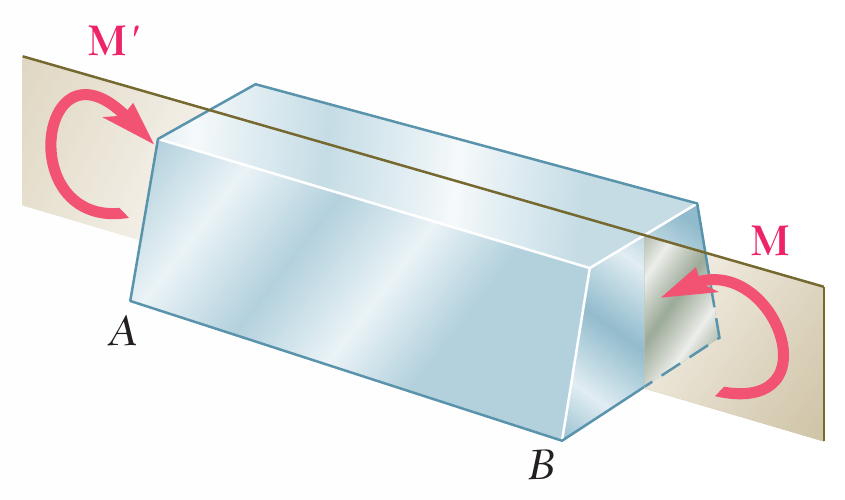
\includegraphics[width=0.48\linewidth,height=2.9cm,keepaspectratio]{Chap_4/fig_4_1.png}\hfill
      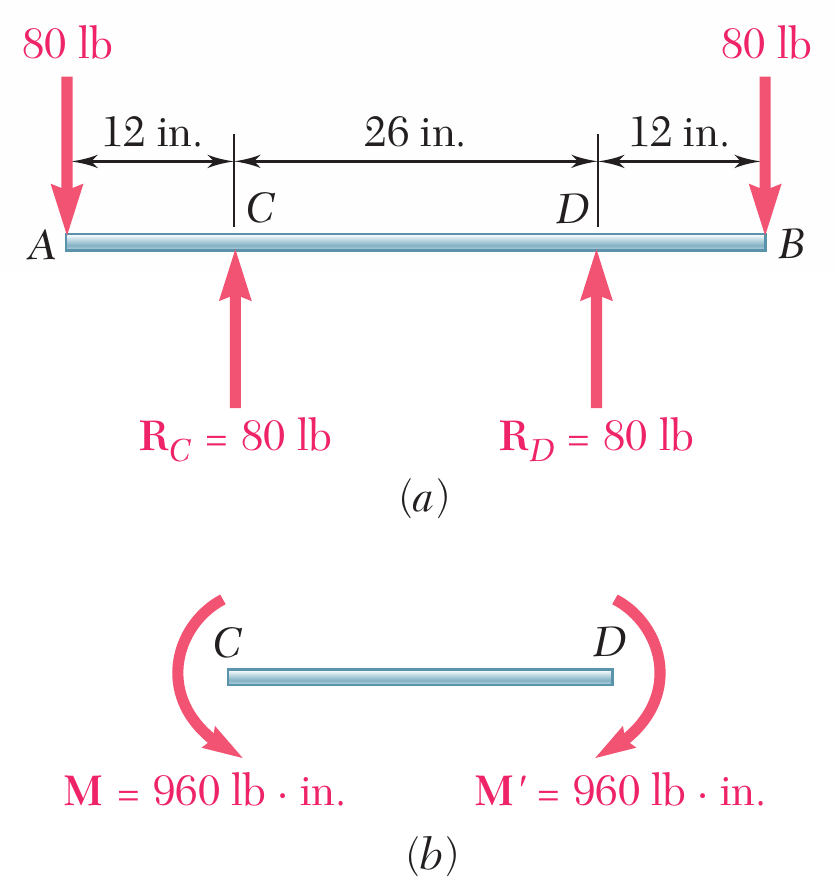
\includegraphics[width=0.48\linewidth,height=2.9cm,keepaspectratio]{Chap_4/fig_4_2.png}\\[4pt]
      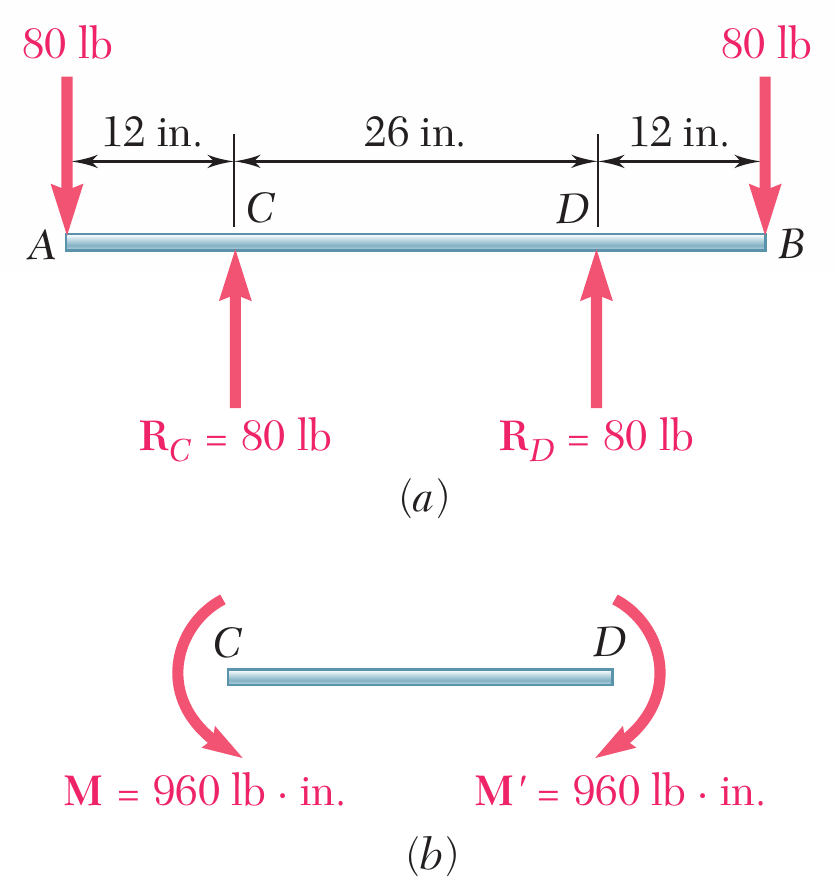
\includegraphics[width=0.7\linewidth,height=2.9cm,keepaspectratio]{Chap_4/fig_4_2.png}
  \end{columns}
\end{frame}
% ===========
\section{Các dạng tải trọng khác}
\begin{frame}[t]{Các dạng tải trọng khác}
  \begin{columns}[T]
    \column{0.58\textwidth}
      \small
      \begin{itemize}
        \setlength{\itemsep}{0.8em}
        \item \textbf{Tải trọng lệch tâm:} lực dọc trục không đi qua trọng
              tâm mặt cắt gây ra nội lực tương đương với một lực dọc trục
              và một ngẫu lực.
        \item \textbf{Tải trọng ngang:} tải trọng ngang tập trung hoặc phân
              bố gây ra nội lực tương đương với một lực cắt và một ngẫu lực.
        \item \textbf{Nguyên lý cộng tác dụng:} ứng suất pháp do uốn thuần
              túy có thể được tổ hợp với ứng suất pháp do lực dọc trục và
              ứng suất tiếp do lực cắt để tìm trạng thái ứng suất đầy đủ.
      \end{itemize}
    \column{0.40\textwidth}
      \centering
      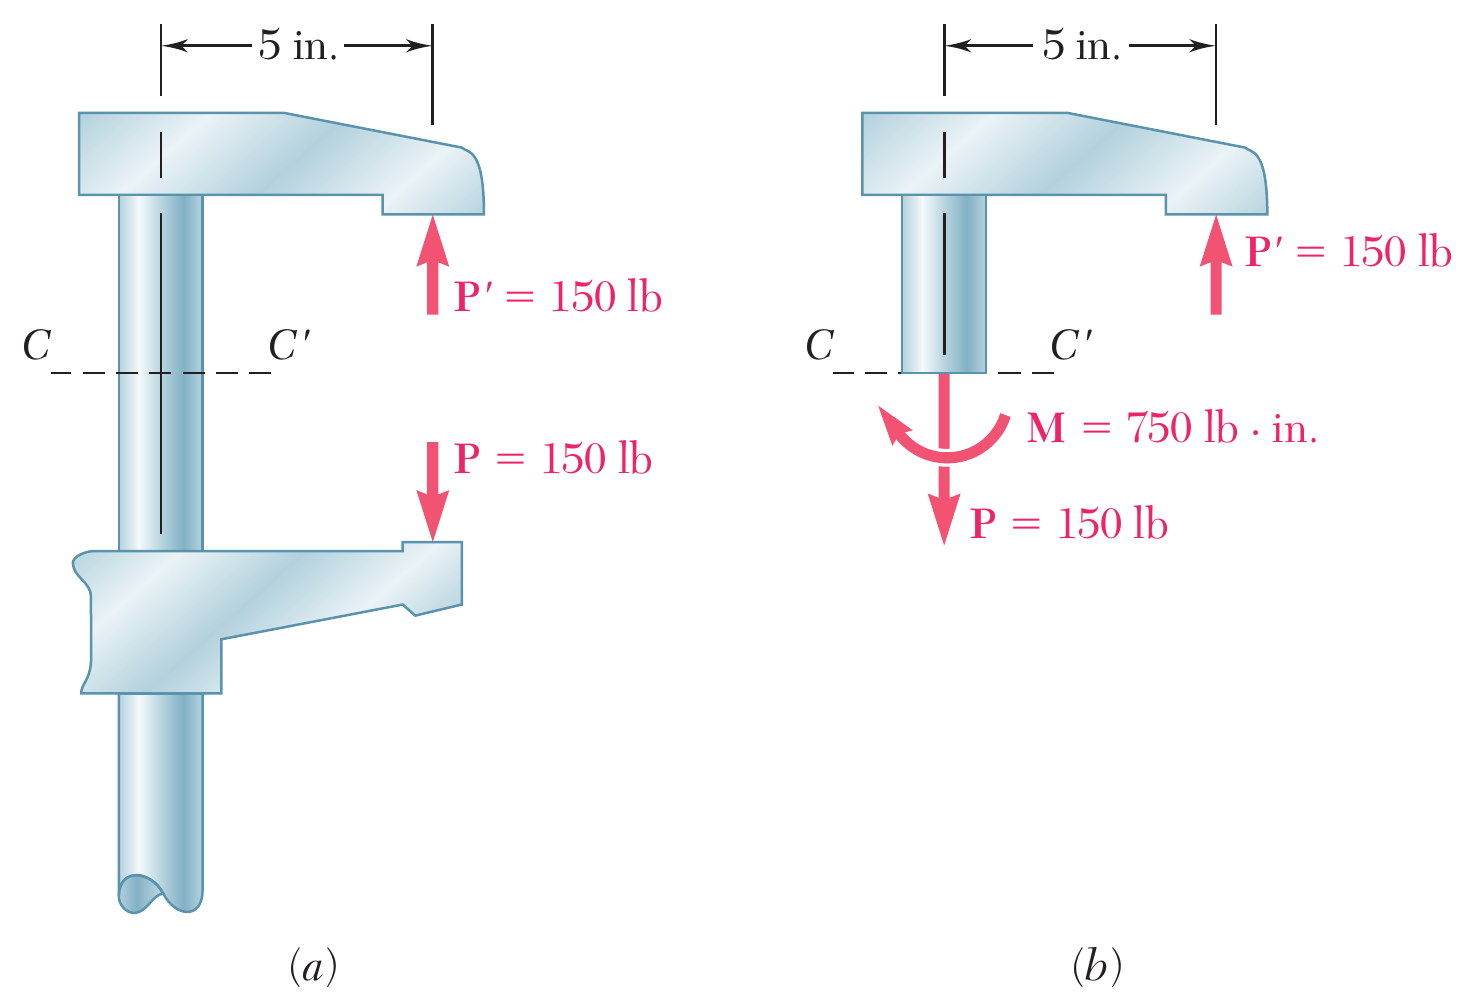
\includegraphics[width=\linewidth,height=5.5cm,keepaspectratio]{Chap_4/fig_4_3.png}
  \end{columns}
\end{frame}
% ===========
\section{Cấu kiện đối xứng chịu uốn thuần túy}
\begin{frame}[t]{Cấu kiện đối xứng chịu uốn thuần túy}
  \begin{columns}[T]
    \column{0.60\textwidth}
      \footnotesize
      \begin{itemize}
        \setlength{\itemsep}{0.20em}
        \item Nội lực trên mọi mặt cắt ngang tương đương với một ngẫu lực.
              Mô men của ngẫu lực là mô men uốn của mặt cắt.
        \item Theo tĩnh học, ngẫu lực $M$ gồm hai lực bằng nhau và ngược
              chiều.
        \item Tổng các thành phần của các lực theo mọi phương bằng không.
        \item Mô men là như nhau đối với mọi trục vuông góc với mặt phẳng
              ngẫu lực, và bằng không đối với mọi trục nằm trong mặt phẳng
              đó.
        \item Các yêu cầu này có thể áp dụng cho tổng các thành phần và
              mô men của các nội lực phân tố (siêu tĩnh):
        \[
          F_x = \int\sigma_x\,dA = 0 \qquad
          M_y = \int z\sigma_x\,dA = 0
        \]
        \[
          M_z = \int -y\sigma_x\,dA = M
        \]
      \end{itemize}
    \column{0.38\textwidth}
      \centering
      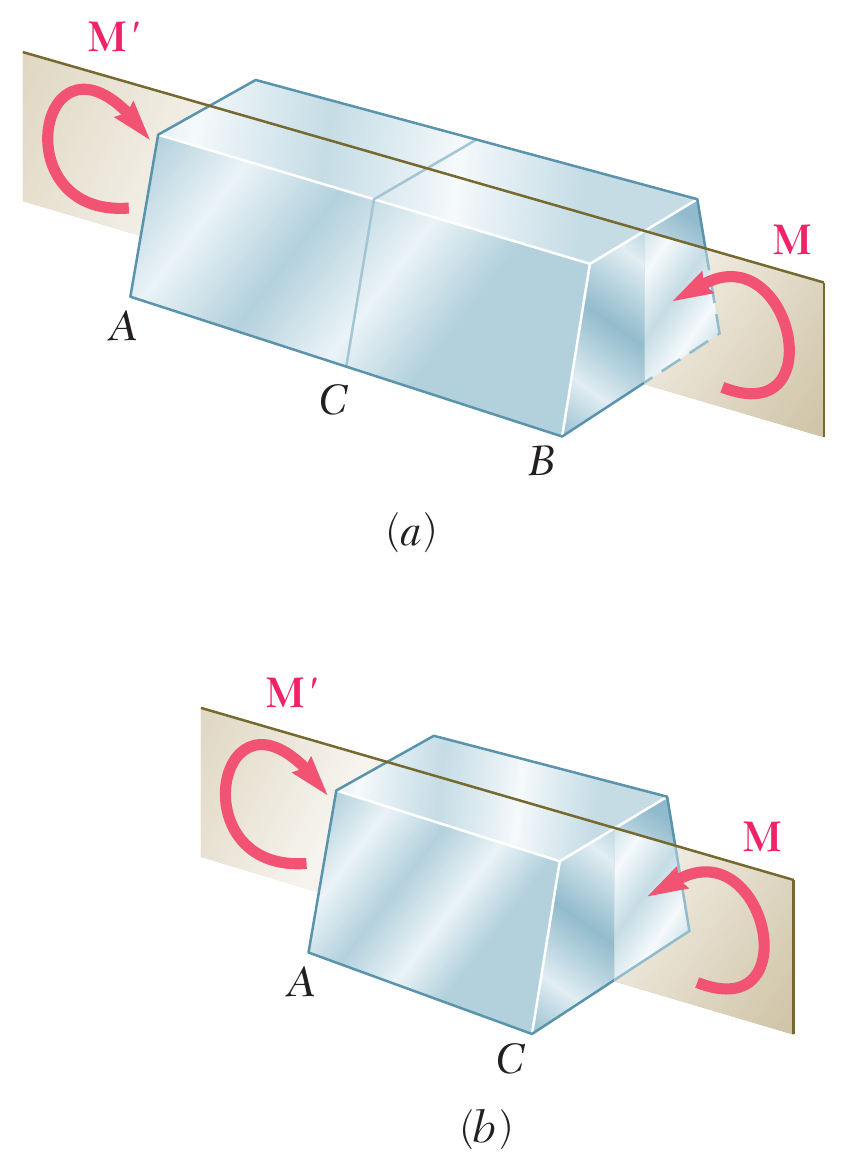
\includegraphics[width=\linewidth,height=2.5cm,keepaspectratio]{Chap_4/fig_4_5.png}\\[2pt]
      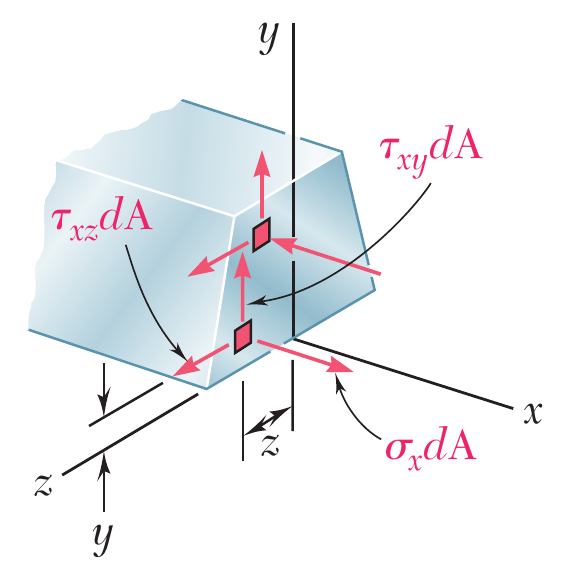
\includegraphics[width=\linewidth,height=2.5cm,keepaspectratio]{Chap_4/fig_4_6.png}
  \end{columns}
\end{frame}
% ===========
\section{Biến dạng khi uốn}
\begin{frame}[t]{Biến dạng khi uốn}
  \begin{columns}[T]
    \column{0.58\textwidth}
      \small
      Dầm có mặt phẳng đối xứng chịu uốn thuần túy:
      \begin{itemize}
        \setlength{\itemsep}{0.3em}
        \item cấu kiện vẫn đối xứng
        \item bị uốn đều thành một cung tròn
        \item mặt cắt ngang đi qua tâm cung và vẫn phẳng
        \item chiều dài thớ trên giảm và chiều dài thớ dưới tăng
        \item phải tồn tại một \emph{mặt trung hòa} song song với mặt trên
              và mặt dưới, có chiều dài không thay đổi
        \item ứng suất và biến dạng âm (nén) ở phía trên mặt trung hòa và
              dương (kéo) ở phía dưới
      \end{itemize}
    \column{0.40\textwidth}
      \centering
      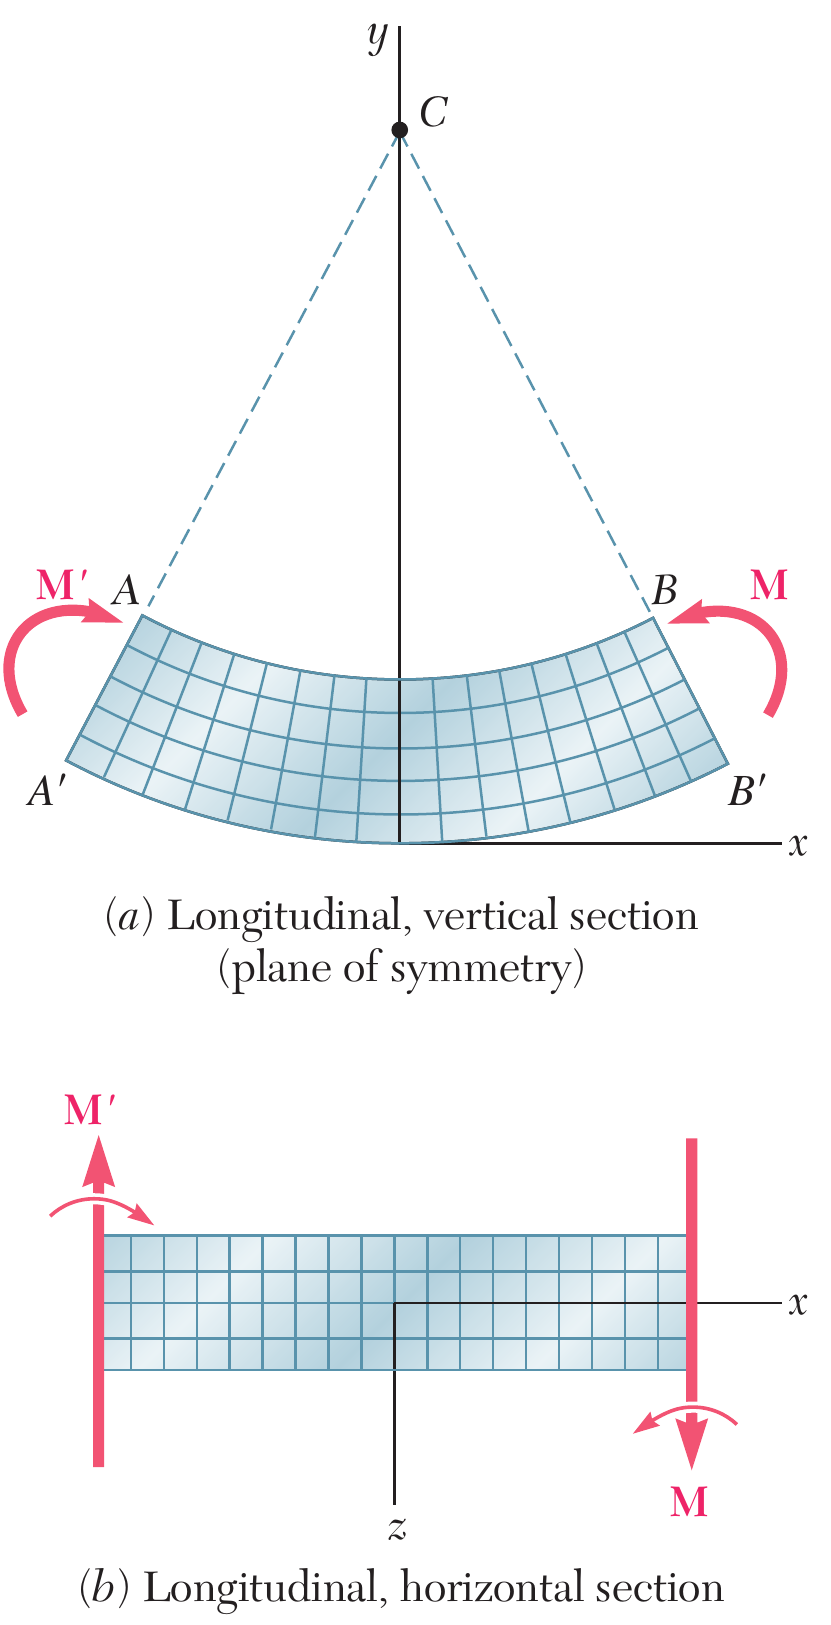
\includegraphics[width=\linewidth,height=5.5cm,keepaspectratio]{Chap_4/fig_4_9.png}
  \end{columns}
\end{frame}
% ===========
\section{Biến dạng do uốn}
\begin{frame}[t]{Biến dạng tỉ đối do uốn}
  \begin{columns}[T]
    \column{0.58\textwidth}
      \small
      Xét một đoạn dầm có chiều dài $L$.

      Sau biến dạng, chiều dài của mặt trung hòa vẫn là $L$. Tại các thớ
      khác:
      \[
        L' = (\rho - y)\theta
      \]
      \[
        \delta = L' - L = (\rho - y)\theta - \rho\theta = -y\theta
      \]
      \[
        \varepsilon_x = \frac{\delta}{L} = -\frac{y\theta}{\rho\theta}
          = -\frac{y}{\rho}
        \quad\text{(biến dạng thay đổi tuyến tính)}
      \]
      \[
        \varepsilon_m = \frac{c}{\rho}
        \quad\text{hay}\quad \rho = \frac{c}{\varepsilon_m}
      \]
      \[
        \varepsilon_x = -\frac{y}{c}\varepsilon_m
      \]
    \column{0.40\textwidth}
      \centering
      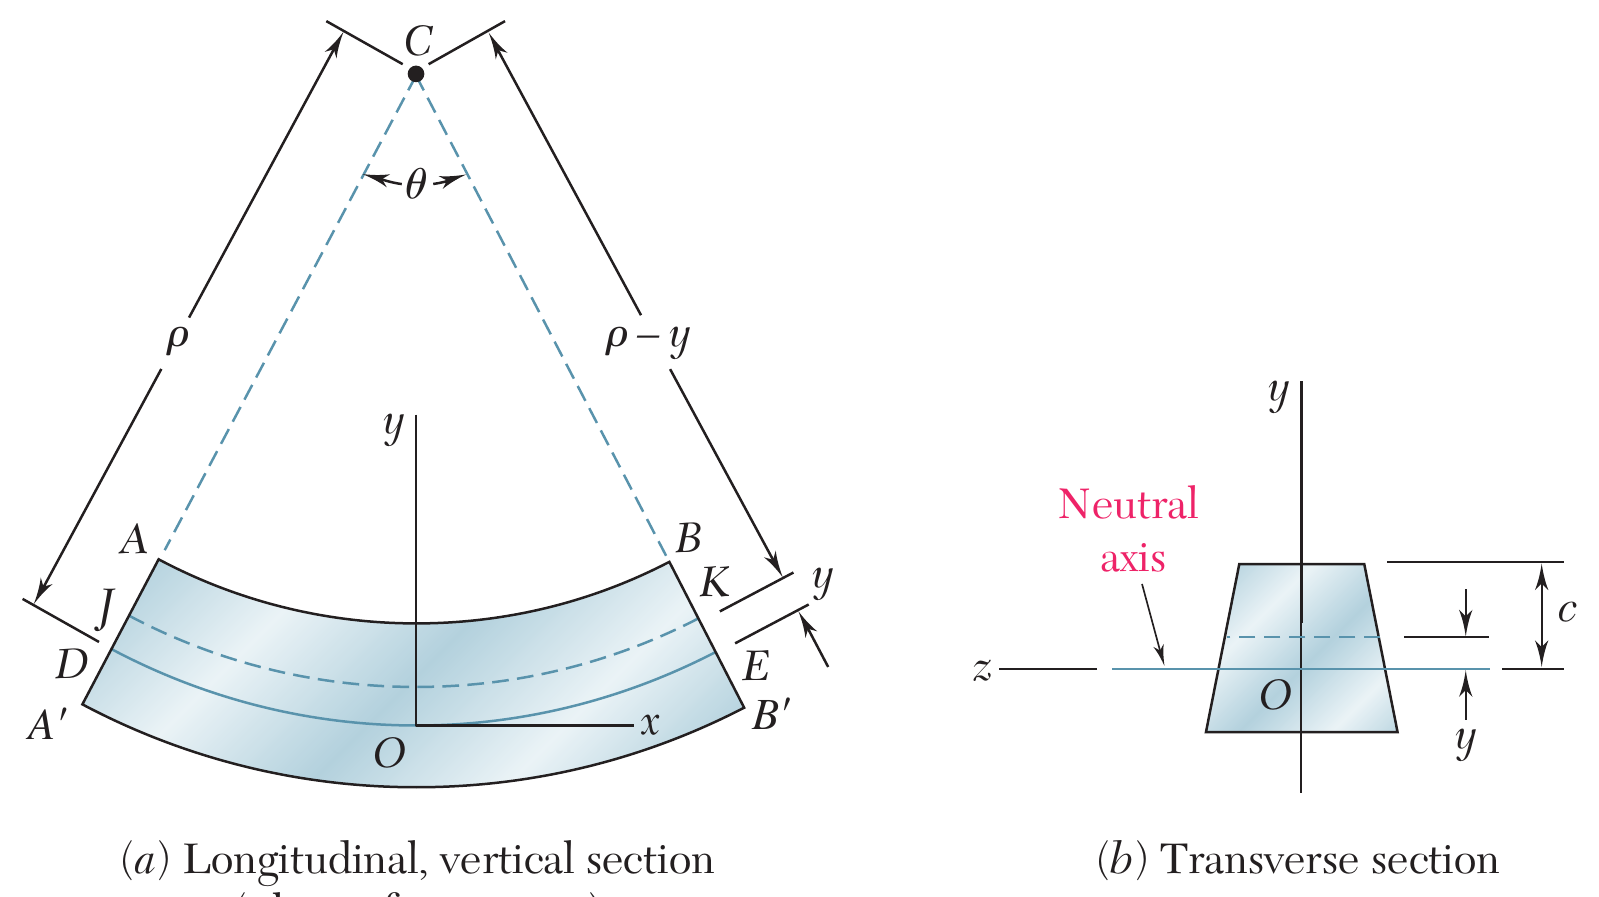
\includegraphics[width=\linewidth,height=2.9cm,keepaspectratio]{Chap_4/fig_4_10.png}\\[2pt]
      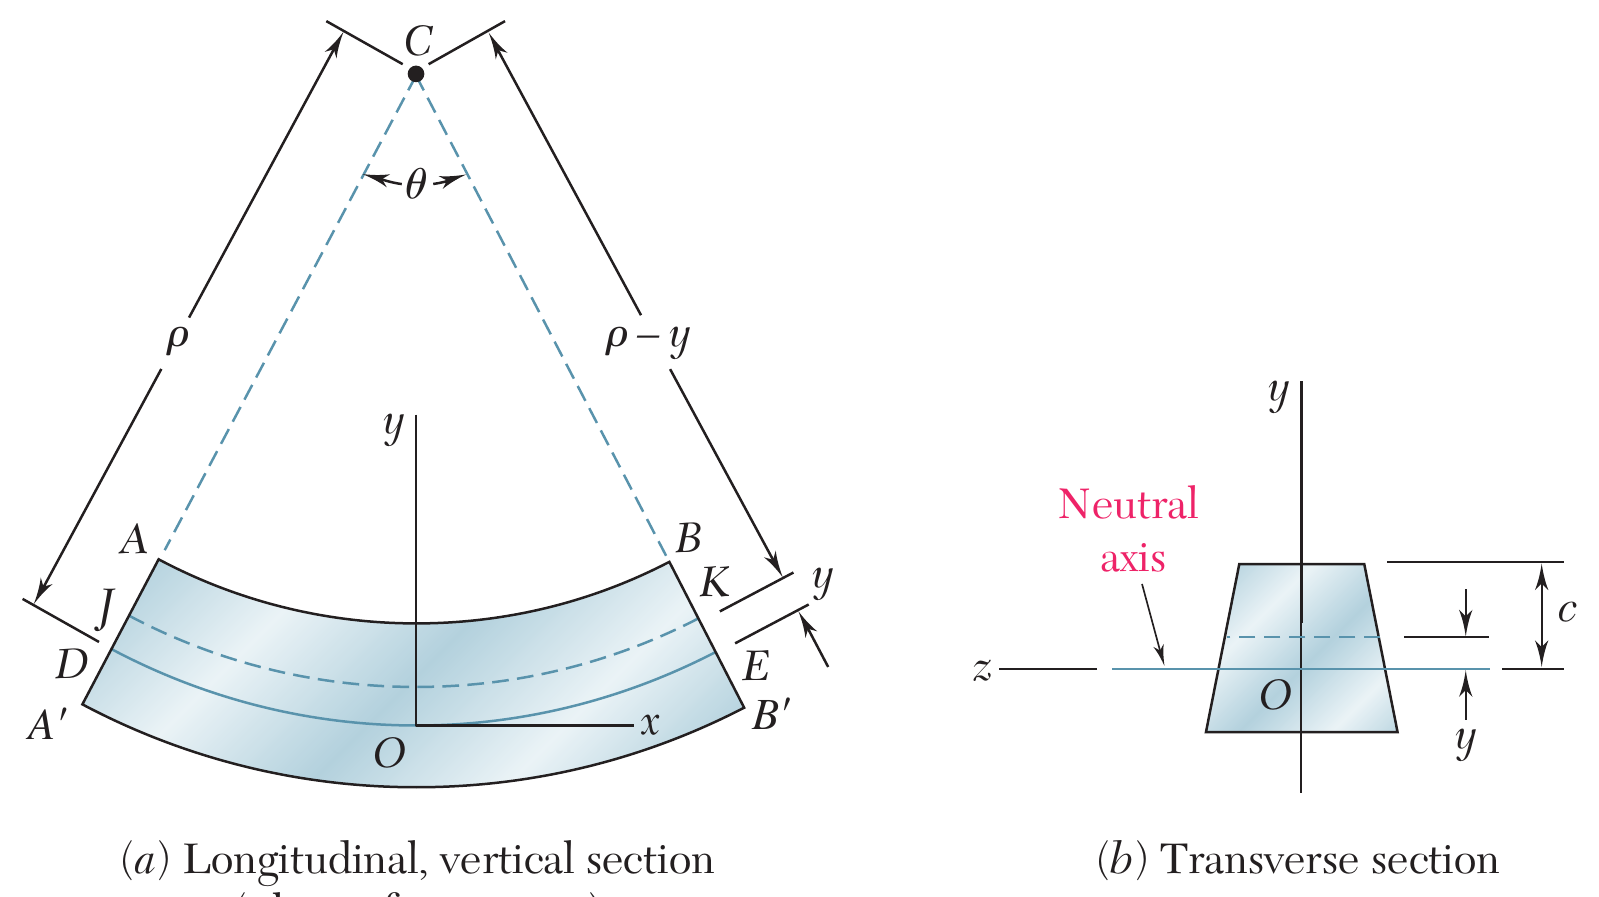
\includegraphics[width=\linewidth,height=2.9cm,keepaspectratio]{Chap_4/fig_4_10.png}
  \end{columns}
\end{frame}
% ===========
\section{Ứng suất do uốn}
\begin{frame}[t]{Ứng suất do uốn}
  \begin{columns}[T]
    \column{0.62\textwidth}
      \scriptsize
      \begin{itemize}
        \setlength{\itemsep}{0.15em}
        \item Với vật liệu đàn hồi tuyến tính:
        \[
          \sigma_x = E\varepsilon_x = -\frac{y}{c}E\varepsilon_m
            = -\frac{y}{c}\sigma_m
          \quad\text{(ứng suất thay đổi tuyến tính)}
        \]
        \item Điều kiện cân bằng tĩnh học:
        \[
          F_x = 0 = \int\sigma_x\,dA = \int -\frac{y}{c}\sigma_m\,dA
          \quad\Rightarrow\quad
          0 = -\frac{\sigma_m}{c}\int y\,dA
        \]
        Mô men tĩnh đối với mặt trung hòa bằng không. Do đó, mặt trung hòa
        phải đi qua trọng tâm mặt cắt.
        \item Điều kiện cân bằng tĩnh học:
        \[
          M = \int(-y\sigma_x\,dA) = \int(-y)\left(-\frac{y}{c}\sigma_m\right)dA
            = \frac{\sigma_m}{c}\int y^2\,dA = \frac{\sigma_mI}{c}
        \]
        \[
          \sigma_m = \frac{Mc}{I} = \frac{M}{S}
        \]
        Thay vào $\sigma_x = -\dfrac{y}{c}\sigma_m$:
        \[
          \sigma_x = -\frac{My}{I}
        \]
      \end{itemize}
    \column{0.36\textwidth}
      \centering
      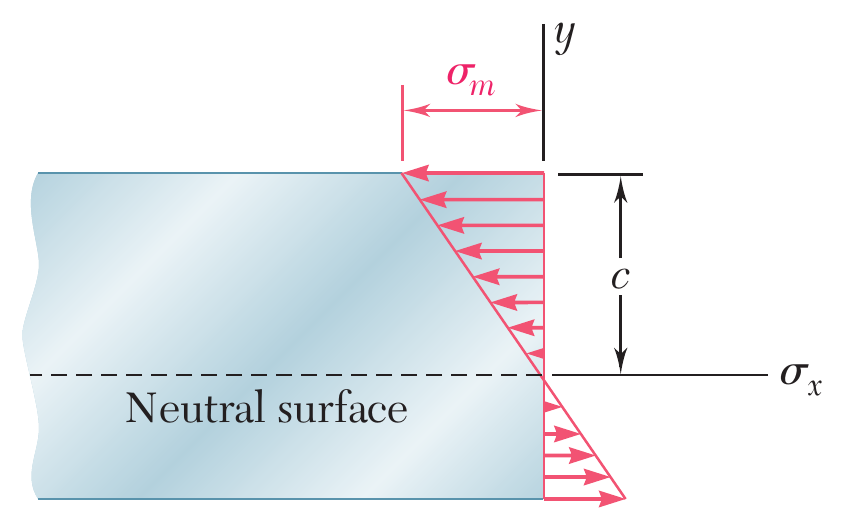
\includegraphics[width=\linewidth,height=4.7cm,keepaspectratio]{Chap_4/fig_4_11.png}
  \end{columns}
\end{frame}
% ===========
\section{Đặc trưng hình học của mặt cắt dầm}
\begin{frame}[t]{Đặc trưng hình học của mặt cắt dầm}
  \begin{columns}[T]
    \column{0.62\textwidth}
      \footnotesize
      \begin{itemize}
        \setlength{\itemsep}{0.20em}
        \item Ứng suất pháp lớn nhất do uốn:
        \[
          \sigma_m = \frac{Mc}{I} = \frac{M}{S}
        \]
        $I$ = mô men quán tính của mặt cắt\\
        $S = \dfrac{I}{c}$ = mô men chống uốn

        Mặt cắt dầm có mô men chống uốn lớn hơn sẽ có ứng suất lớn nhất
        nhỏ hơn.
        \item Xét mặt cắt dầm hình chữ nhật:
        \[
          S = \frac{I}{c} = \frac{\frac{1}{12}bh^3}{h/2}
            = \tfrac{1}{6}bh^2 = \tfrac{1}{6}Ah
        \]
        Giữa hai dầm có cùng diện tích mặt cắt, dầm có chiều cao lớn hơn
        sẽ chịu uốn hiệu quả hơn.
        \item Dầm thép kết cấu được thiết kế để có mô men chống uốn lớn.
      \end{itemize}
    \column{0.36\textwidth}
      \centering
      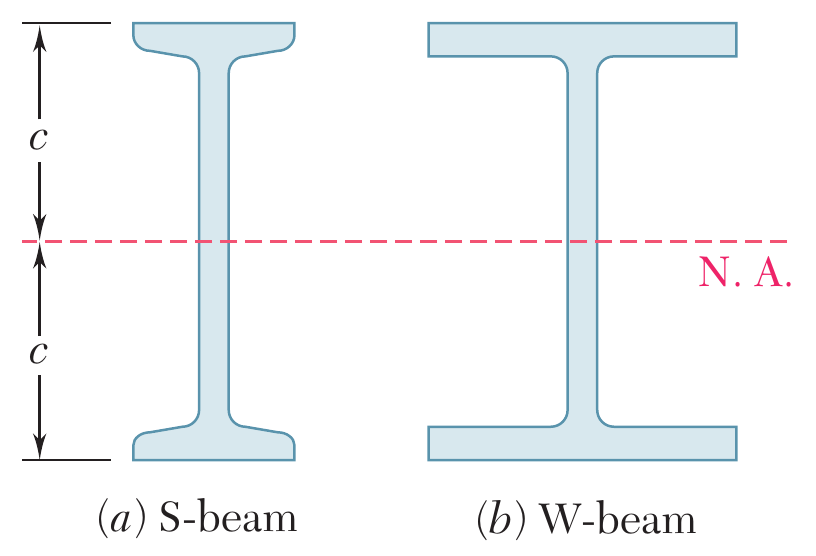
\includegraphics[width=\linewidth,height=4.7cm,keepaspectratio]{Chap_4/fig_4_13.png}
  \end{columns}
\end{frame}
% ===========
\section{Đặc trưng của các thép hình tiêu chuẩn}
\begin{frame}[t]{Đặc trưng của các thép hình tiêu chuẩn Mỹ}
  \centering
  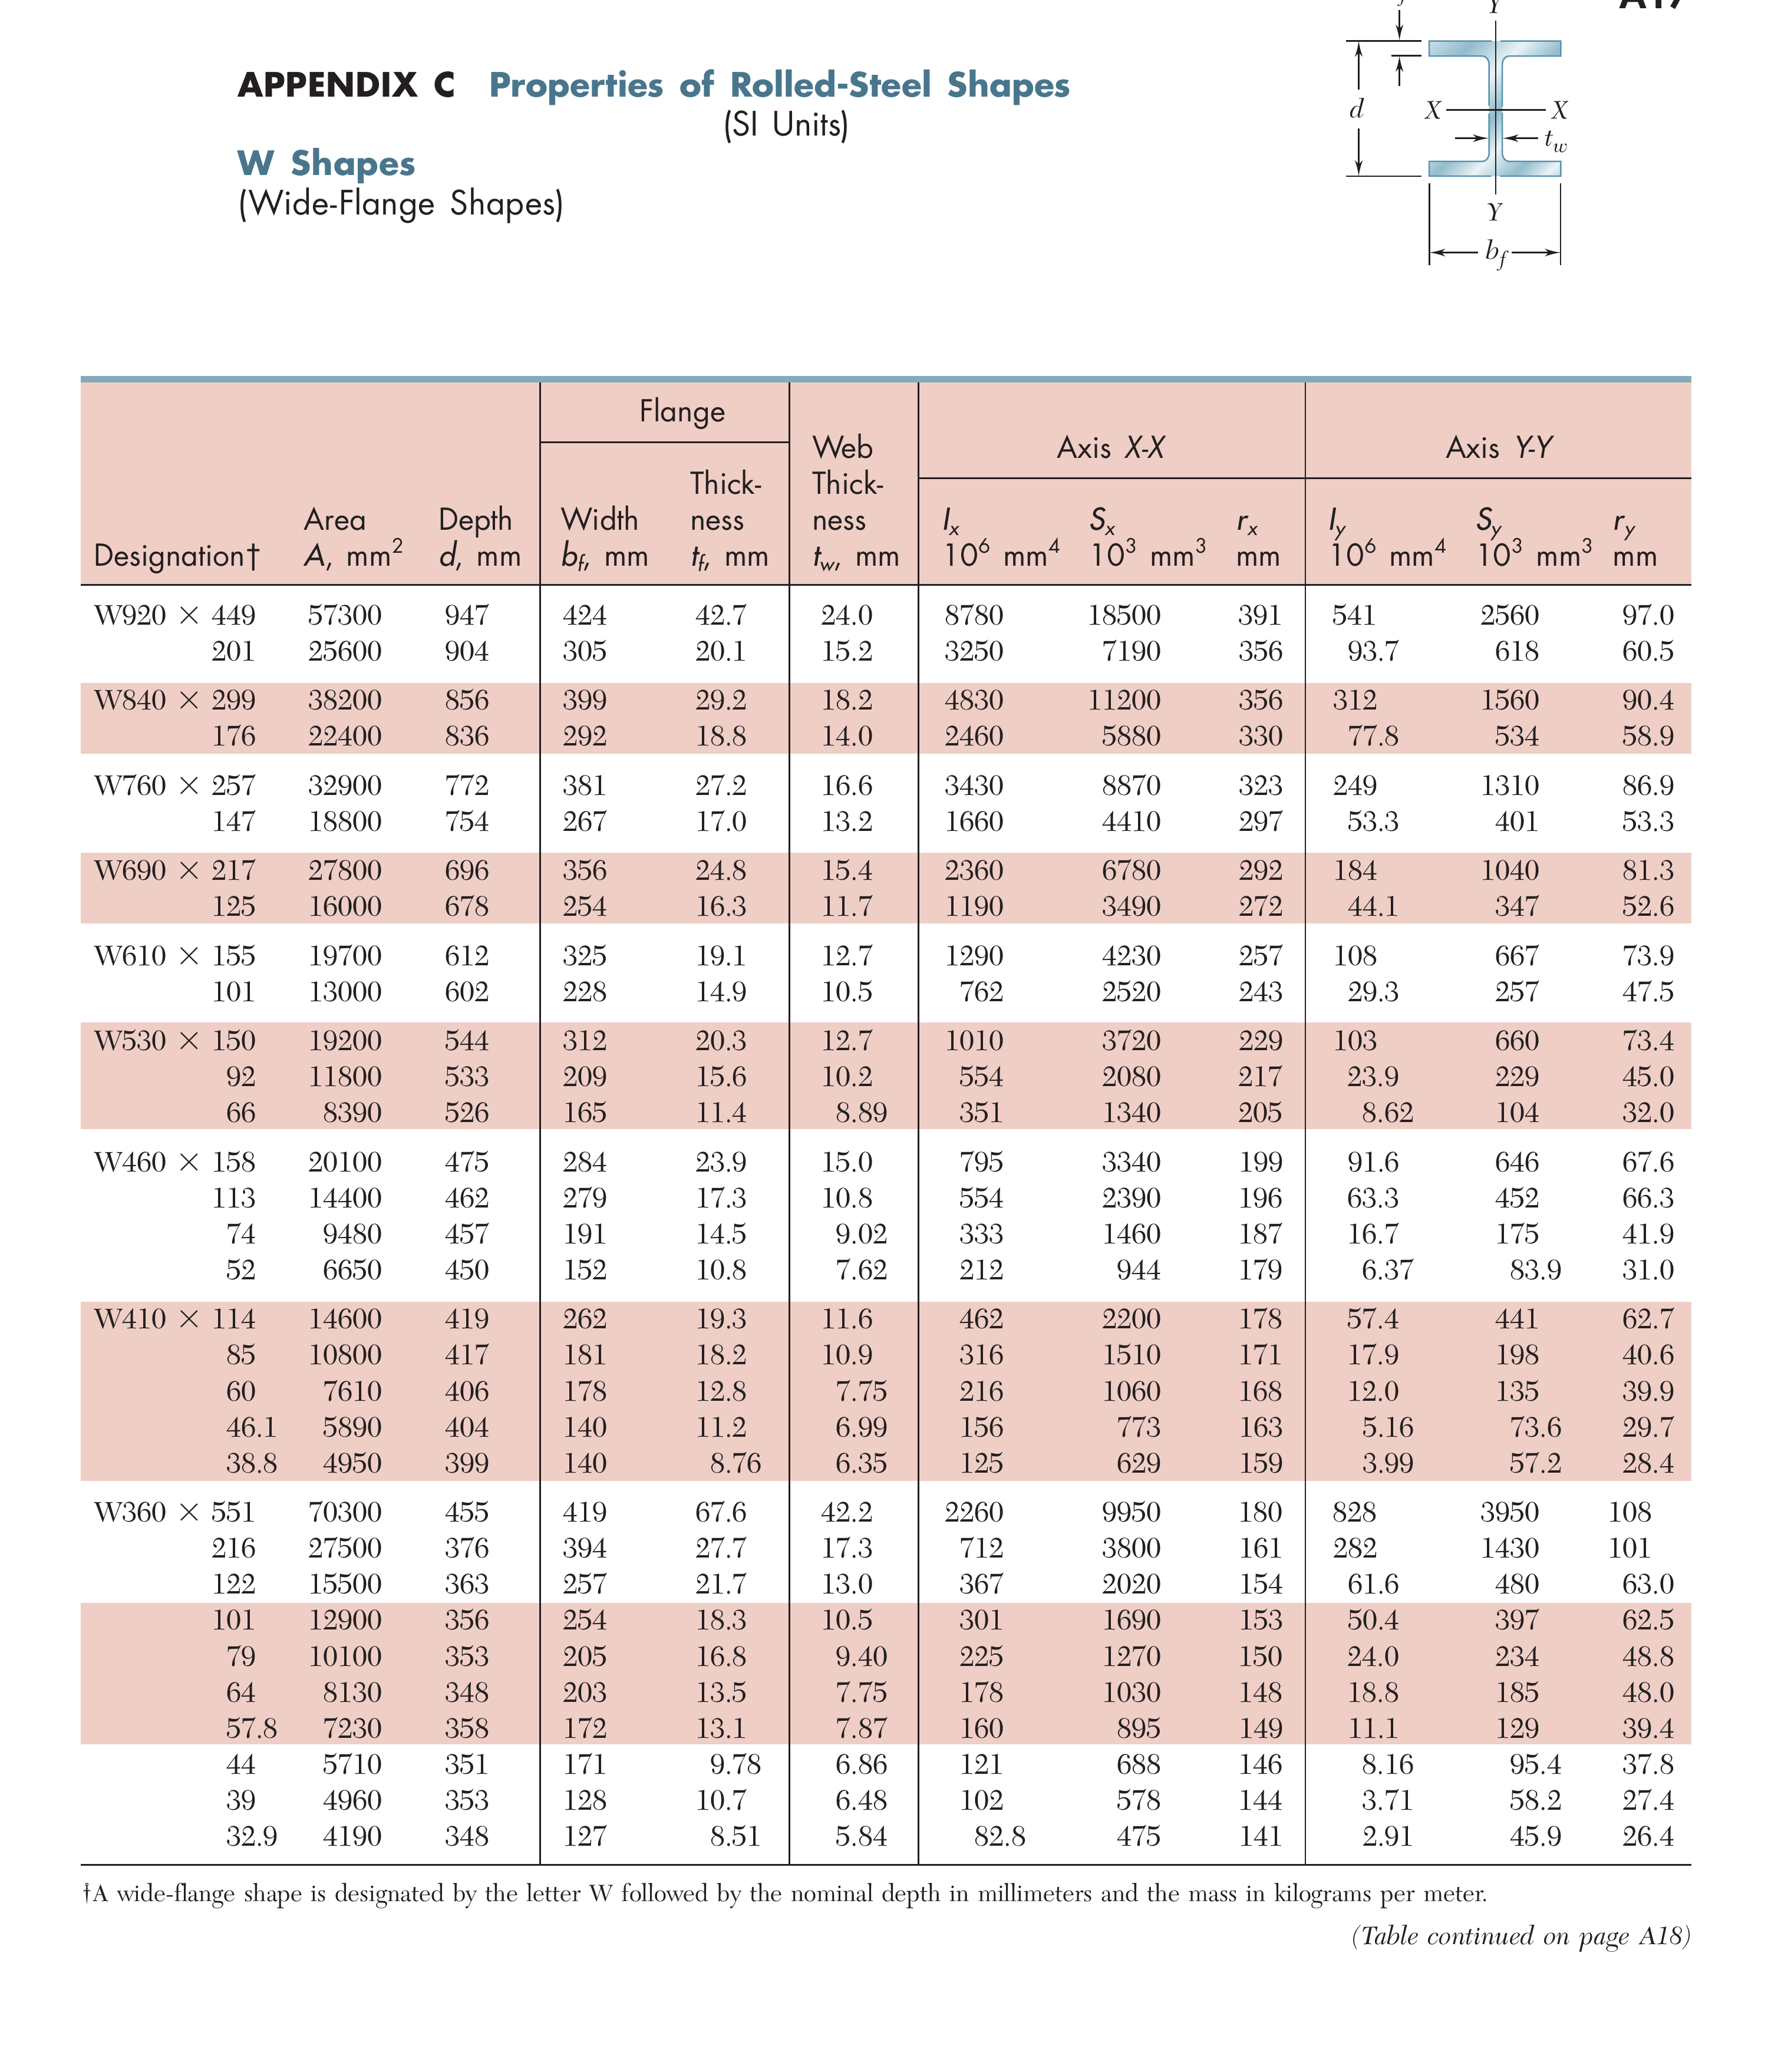
\includegraphics[width=0.9\textwidth,height=6.5cm,keepaspectratio]{Chap_4/appendix_C_W_shapes_SI.png}
\end{frame}
% ===========
\section{Biến dạng trong mặt cắt ngang}
\begin{frame}[t]{Biến dạng trong mặt cắt ngang}
  \begin{columns}[T]
    \column{0.60\textwidth}
      \small
      \begin{itemize}
        \setlength{\itemsep}{0.5em}
        \item Biến dạng do mô men uốn $M$ được đặc trưng bởi độ cong của
              mặt trung hòa:
        \[
          \frac{1}{\rho} = \frac{\varepsilon_m}{c} = \frac{\sigma_m}{Ec}
            = \frac{1}{Ec}\frac{Mc}{I} = \frac{M}{EI}
        \]
        \item Mặc dù mặt cắt ngang vẫn phẳng khi chịu mô men uốn, biến dạng
              trong mặt phẳng mặt cắt khác không:
        \[
          \varepsilon_y = -\nu\varepsilon_x = \frac{\nu y}{\rho}
          \qquad
          \varepsilon_z = -\nu\varepsilon_x = \frac{\nu y}{\rho}
        \]
        \item Sự giãn ra phía trên mặt trung hòa và co lại phía dưới gây ra
              độ cong trong mặt phẳng mặt cắt:
        \[
          \frac{1}{\rho'} = \frac{\nu}{\rho} = \text{độ cong phản đối (anticlastic)}
        \]
      \end{itemize}
    \column{0.38\textwidth}
      \centering
      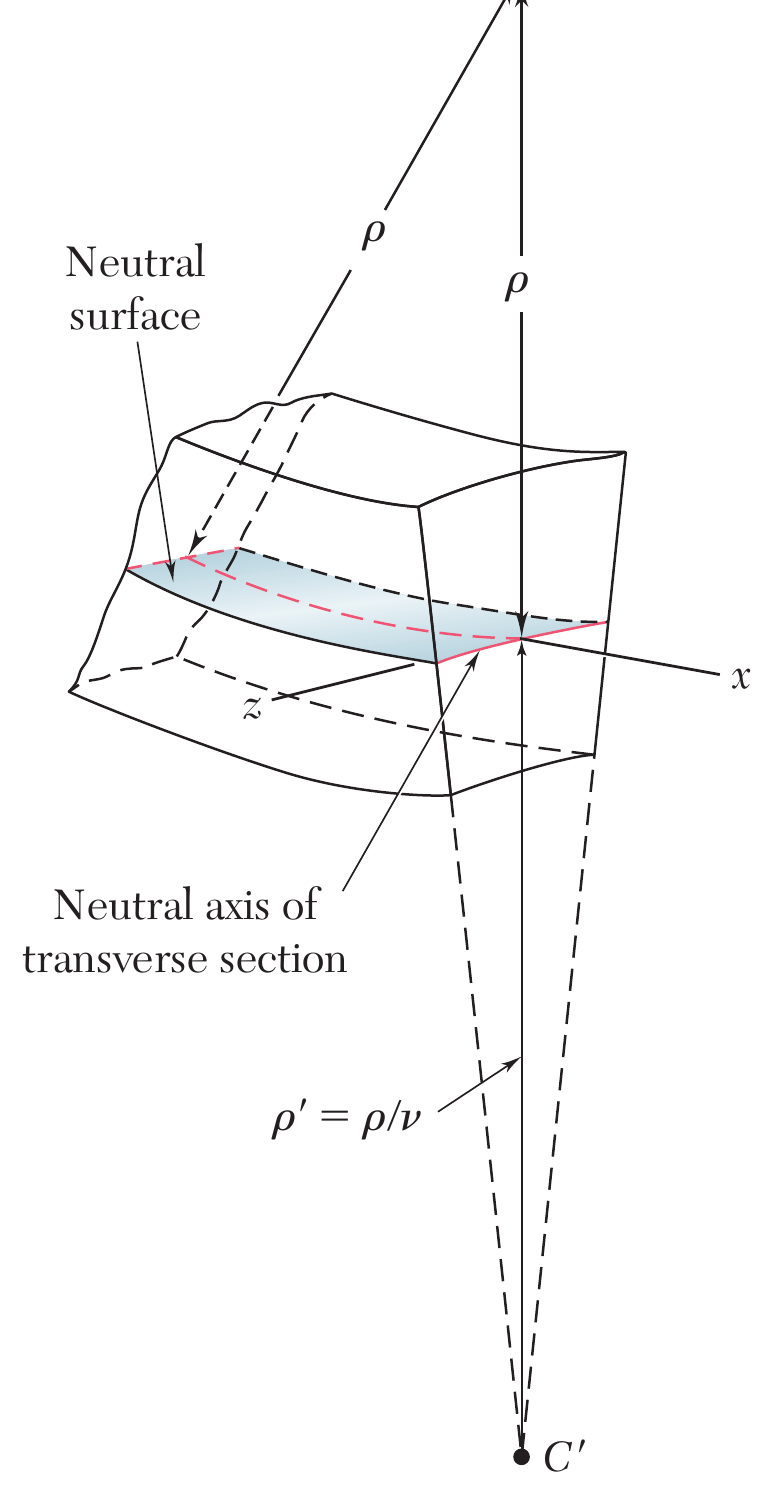
\includegraphics[width=\linewidth,height=5.5cm,keepaspectratio]{Chap_4/fig_4_18.png}
  \end{columns}
\end{frame}
% ===========
\section{Bài mẫu 4.2}
\begin{frame}[t]{Bài mẫu 4.2}
  \begin{columns}[T]
    \column{0.40\textwidth}
      \centering
      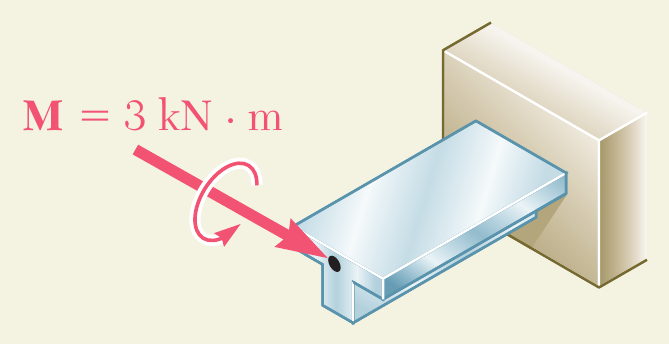
\includegraphics[width=\linewidth,height=2.5cm,keepaspectratio]{Chap_4/sp_4_2_b.png}\\[2pt]
      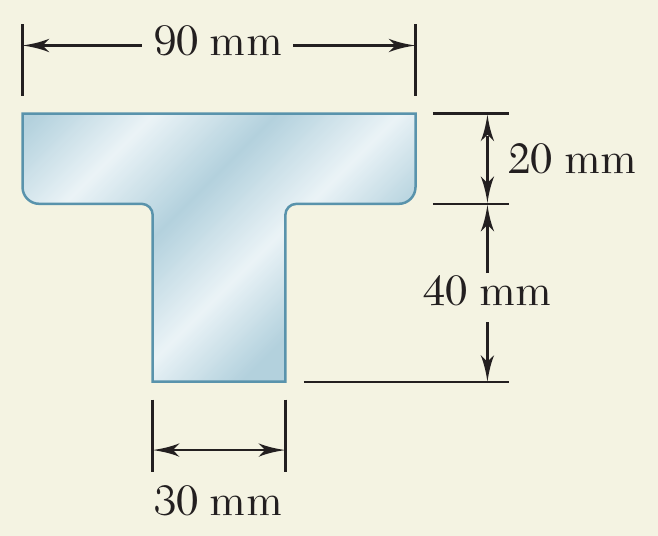
\includegraphics[width=\linewidth,height=2.5cm,keepaspectratio]{Chap_4/sp_4_2_a.png}
    \column{0.58\textwidth}
      \footnotesize
      Một chi tiết máy bằng gang chịu ngẫu lực $3\,\mathrm{kN\cdot m}$.
      Biết $E = 165\,\mathrm{GPa}$ và bỏ qua ảnh hưởng của góc lượn, xác
      định (a) ứng suất kéo và nén lớn nhất, (b) bán kính cong.

      \vspace{0.5em}
      \textbf{LỜI GIẢI:}
      \begin{itemize}
        \setlength{\itemsep}{0.15em}
        \item Từ hình học mặt cắt, tính vị trí trọng tâm và mô men quán
              tính của mặt cắt:
        \[
          \bar{Y} = \frac{\sum\bar{y}A}{\sum A} \qquad
          I_{x'} = \sum\left(\bar{I} + Ad^2\right)
        \]
        \item Áp dụng công thức uốn đàn hồi để tìm ứng suất kéo và nén lớn
              nhất:
        \[
          \sigma_m = \frac{Mc}{I}
        \]
        \item Tính độ cong:
        \[
          \frac{1}{\rho} = \frac{M}{EI}
        \]
      \end{itemize}
  \end{columns}
\end{frame}
% ===========
\begin{frame}[t]{Bài mẫu 4.2 (tiếp)}
  \begin{columns}[T]
    \column{0.60\textwidth}
      \small
      \textbf{LỜI GIẢI:} Từ hình học mặt cắt, tính vị trí trọng tâm và mô
      men quán tính.
      \vspace{0.3em}
      \begin{center}
        \footnotesize
        \setlength{\tabcolsep}{3pt}\begin{tabular}{cccc}
          \hline
          & Diện tích, $\mathrm{mm}^2$ & $\bar{y}$, mm & $\bar{y}A$, $\mathrm{mm}^3$\\
          \hline
          1 & $20\times90 = 1800$ & 50 & $90\times10^{3}$\\
          2 & $40\times30 = 1200$ & 20 & $24\times10^{3}$\\
          \hline
          & $\sum A = 3000$ & & $\sum\bar{y}A = 114\times10^{3}$\\
          \hline
        \end{tabular}
      \end{center}
      \[
        \bar{Y} = \frac{\sum\bar{y}A}{\sum A} = \frac{114\times10^{3}}{3000}
          = 38\,\mathrm{mm}
      \]
      \[
        I_{x'} = \sum\left(\bar{I} + Ad^2\right)
          = \sum\left(\tfrac{1}{12}bh^3 + Ad^2\right)
      \]
      \[
        = \left(\tfrac{1}{12}90\times20^3 + 1800\times12^2\right)
      \]
      \[
        \quad + \left(\tfrac{1}{12}30\times40^3 + 1200\times18^2\right)
      \]
      \[
        I = 868\times10^{3}\,\mathrm{mm}^4 = 868\times10^{-9}\,\mathrm{m}^4
      \]
    \column{0.38\textwidth}
      \centering
      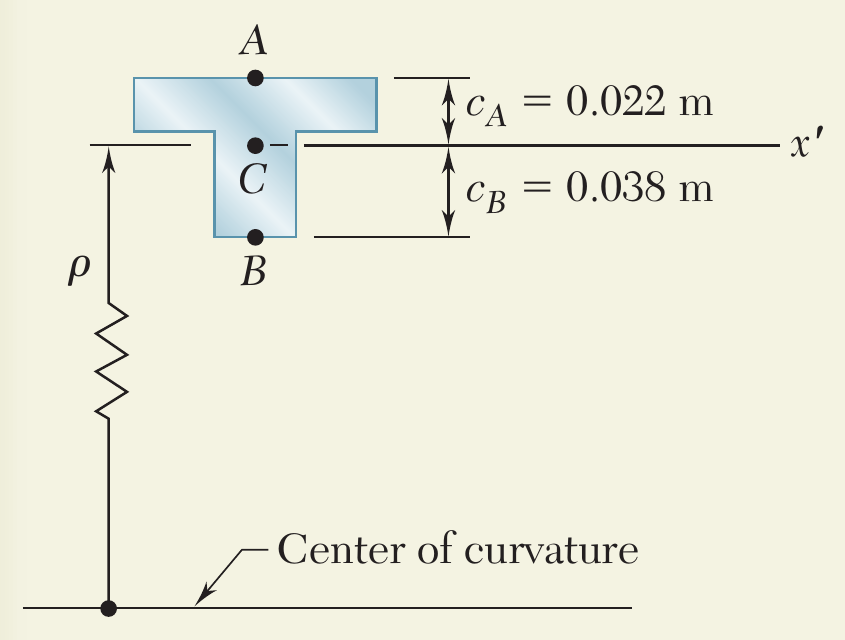
\includegraphics[width=\linewidth,height=5.5cm,keepaspectratio]{Chap_4/sp_4_2_c.png}
  \end{columns}
\end{frame}
% ===========
\begin{frame}[t]{Bài mẫu 4.2 (tiếp)}
  \begin{columns}[T]
    \column{0.60\textwidth}
      \footnotesize
      \begin{itemize}
        \setlength{\itemsep}{0.25em}
        \item Áp dụng công thức uốn đàn hồi để tìm ứng suất kéo và nén lớn
              nhất:
        \[
          \sigma_m = \frac{Mc}{I}
        \]
        \[
          \sigma_A = \frac{Mc_A}{I}
            = \frac{(3\times10^{3})(0{,}022)}{868\times10^{-9}}
          \qquad \boxed{\sigma_A = +76{,}0\,\mathrm{MPa}}
        \]
        \[
          \sigma_B = -\frac{Mc_B}{I}
            = -\frac{(3\times10^{3})(0{,}038)}{868\times10^{-9}}
          \qquad \boxed{\sigma_B = -131{,}3\,\mathrm{MPa}}
        \]
        \item Tính độ cong:
        \[
          \frac{1}{\rho} = \frac{M}{EI}
            = \frac{3\times10^{3}}{(165\times10^{9})(868\times10^{-9})}
        \]
        \[
          \frac{1}{\rho} = 20{,}95\times10^{-3}\,\mathrm{m}^{-1}
        \]
        \[
          \boxed{\rho = 47{,}7\,\mathrm{m}}
        \]
      \end{itemize}
    \column{0.38\textwidth}
      \centering
      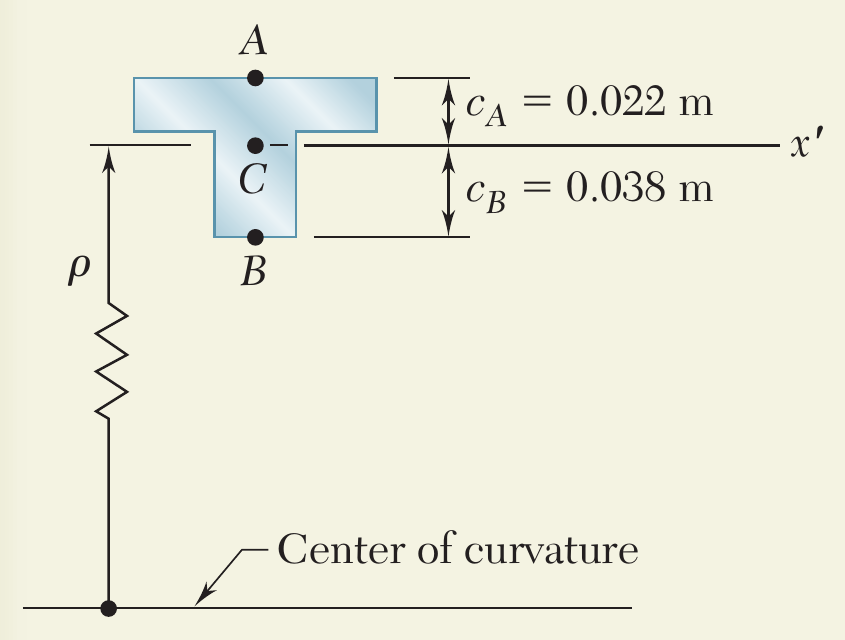
\includegraphics[width=\linewidth,height=4.7cm,keepaspectratio]{Chap_4/sp_4_2_c.png}
  \end{columns}
\end{frame}
% ===========
\section{Uốn cấu kiện làm từ nhiều vật liệu}
\begin{frame}[t]{Uốn cấu kiện làm từ nhiều vật liệu}
  \begin{columns}[T]
    \column{0.62\textwidth}
      \footnotesize
      \begin{itemize}
        \setlength{\itemsep}{0.3em}
        \item Xét dầm composite làm từ hai vật liệu có mô đun $E_1$ và $E_2$.
        \item Biến dạng dài thay đổi tuyến tính:
              $\displaystyle \varepsilon_x = -\frac{y}{\rho}$
        \item Ứng suất pháp thay đổi tuyến tính từng đoạn:
        \[
          \sigma_1 = E_1\varepsilon_x = -\frac{E_1y}{\rho}
          \qquad
          \sigma_2 = E_2\varepsilon_x = -\frac{E_2y}{\rho}
        \]
        Trục trung hòa không đi qua trọng tâm của mặt cắt composite.
        \item Các lực phân tố trên mặt cắt:
        \[
          dF_1 = \sigma_1\,dA = -\frac{E_1y}{\rho}\,dA
          \qquad
          dF_2 = \sigma_2\,dA = -\frac{E_2y}{\rho}\,dA
        \]
        \item Định nghĩa mặt cắt quy đổi sao cho:
        \[
          dF_2 = -\frac{(nE_1)y}{\rho}\,dA = -\frac{E_1y}{\rho}(n\,dA)
          \qquad n = \frac{E_2}{E_1}
        \]
        \[
          \sigma_x = -\frac{My}{I} \qquad
          \sigma_1 = \sigma_x \qquad \sigma_2 = n\sigma_x
        \]
      \end{itemize}
    \column{0.36\textwidth}
      \centering
      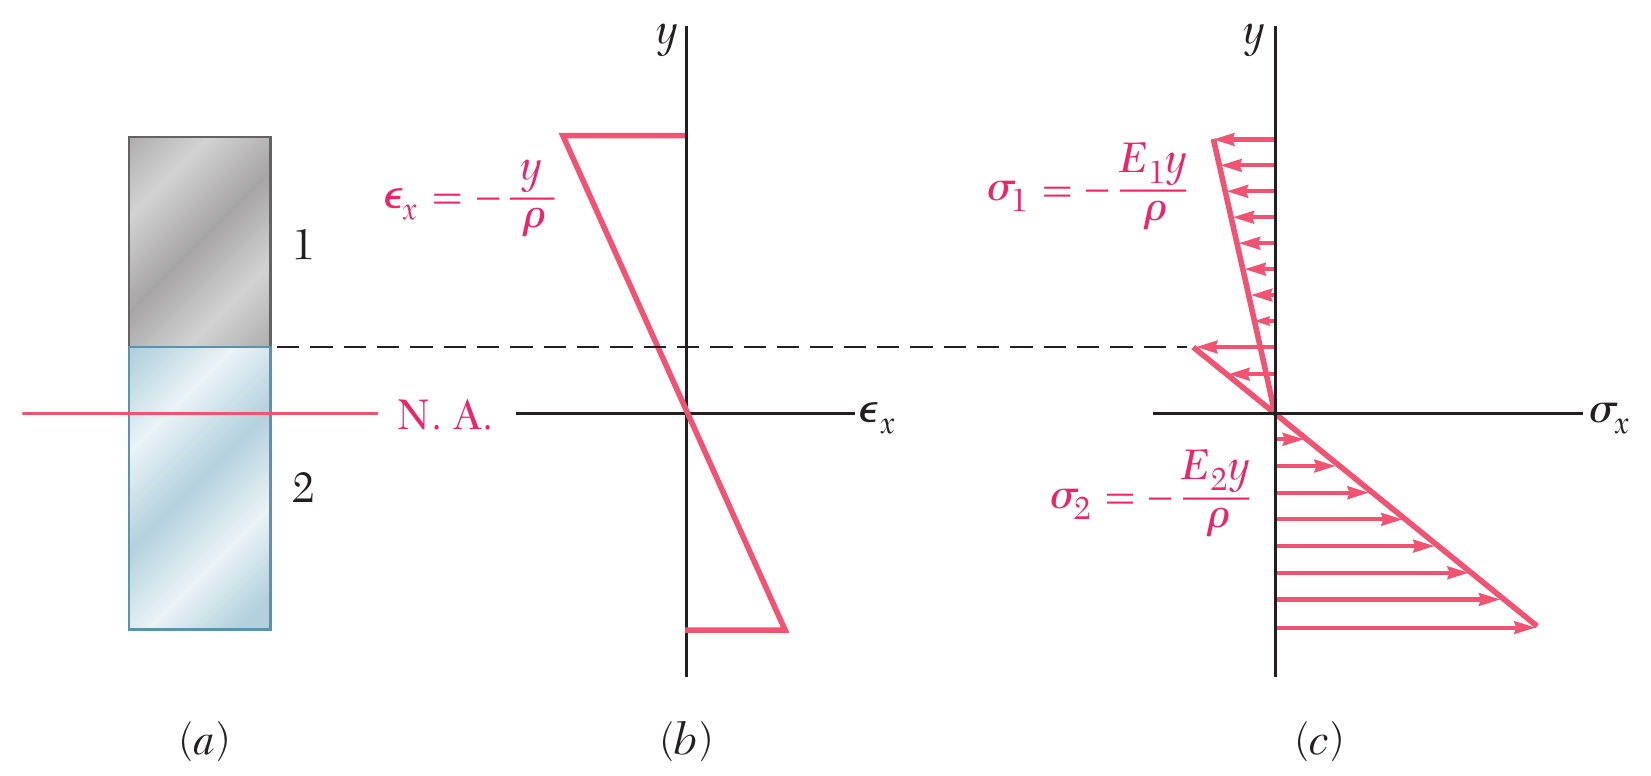
\includegraphics[width=\linewidth,height=2.9cm,keepaspectratio]{Chap_4/fig_4_21.png}\\[2pt]
      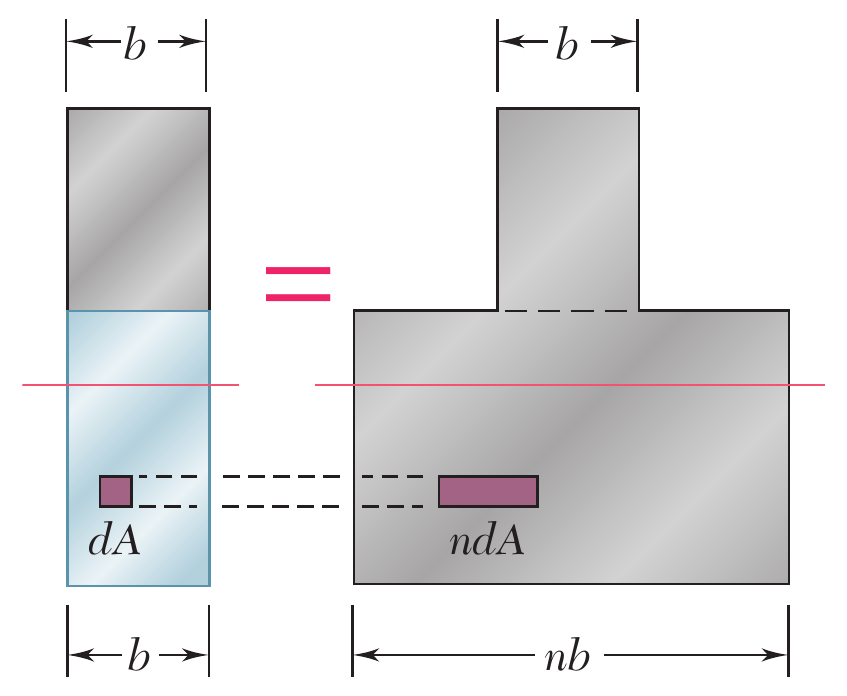
\includegraphics[width=\linewidth,height=2.9cm,keepaspectratio]{Chap_4/fig_4_22.png}
  \end{columns}
\end{frame}
% ===========
\section{Ví dụ 4.03}
\begin{frame}[t]{Ví dụ 4.03}
  \begin{columns}[T]
    \column{0.40\textwidth}
      \centering
      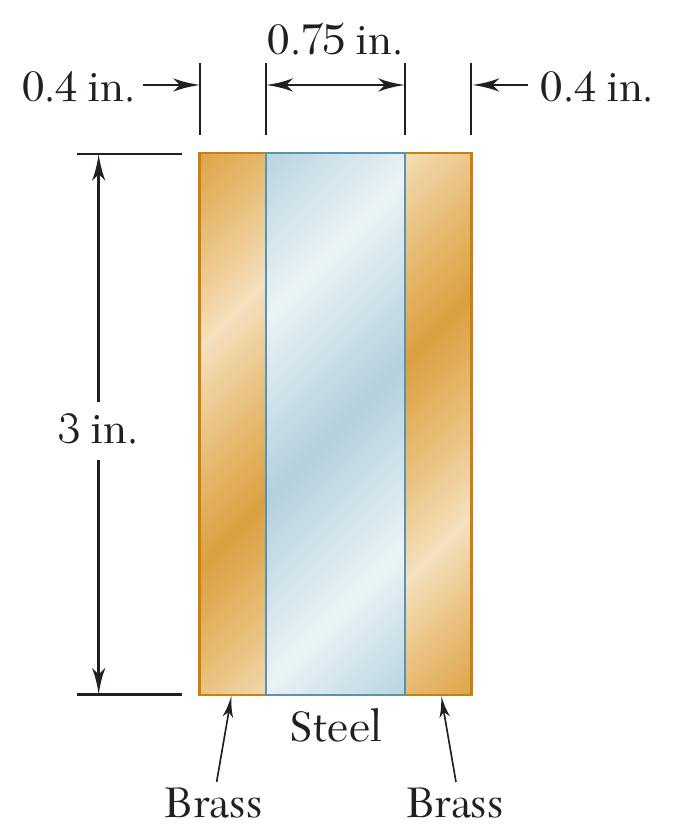
\includegraphics[width=\linewidth,height=5.5cm,keepaspectratio]{Chap_4/fig_4_24.png}
    \column{0.58\textwidth}
      \small
      Một thanh được tạo từ các miếng thép ($E_s = 200\,\mathrm{GPa}$) và
      đồng thau ($E_b = 100\,\mathrm{GPa}$) dán với nhau. Xác định ứng suất
      lớn nhất trong thép và đồng thau khi chịu mô men
      $4{,}5\,\mathrm{kN\cdot m}$.

      \vspace{0.5em}
      \textbf{LỜI GIẢI:}
      \begin{itemize}
        \setlength{\itemsep}{0.3em}
        \item Quy đổi thanh thành mặt cắt tương đương hoàn toàn bằng đồng
              thau.
        \item Tính các đặc trưng hình học của mặt cắt quy đổi.
        \item Tính ứng suất lớn nhất trên mặt cắt quy đổi. Đây chính là ứng
              suất lớn nhất trong các miếng đồng thau.
        \item Xác định ứng suất lớn nhất trong phần thép bằng cách nhân ứng
              suất lớn nhất của mặt cắt quy đổi với tỉ số mô đun đàn hồi.
      \end{itemize}
  \end{columns}
\end{frame}
% ===========
\begin{frame}[t]{Ví dụ 4.03 (tiếp)}
  \begin{columns}[T]
    \column{0.60\textwidth}
      \footnotesize
      \textbf{LỜI GIẢI:}
      \begin{itemize}
        \setlength{\itemsep}{0.25em}
        \item Quy đổi thanh thành mặt cắt tương đương hoàn toàn bằng đồng
              thau:
        \[
          n = \frac{E_s}{E_b} = \frac{200\,\mathrm{GPa}}{100\,\mathrm{GPa}} = 2{,}0
        \]
        \[
          b_T = 10\,\mathrm{mm} + 2\times18\,\mathrm{mm} + 10\,\mathrm{mm}
              = 56\,\mathrm{mm}
        \]
        \item Tính các đặc trưng hình học của mặt cắt quy đổi:
        \[
          I = \tfrac{1}{12}b_Th^3 = \tfrac{1}{12}(56\,\mathrm{mm})(75\,\mathrm{mm})^3
            = 1{,}96875\times10^{6}\,\mathrm{mm}^4
        \]
        \item Tính các ứng suất lớn nhất:
        \[
          \sigma_m = \frac{Mc}{I}
            = \frac{(4500\,\mathrm{N\cdot m})(0{,}0375\,\mathrm{m})}
                   {1{,}96875\times10^{-6}\,\mathrm{m}^4}
            = 85{,}7\,\mathrm{MPa}
        \]
        \[
          (\sigma_b)_{\max} = \sigma_m \qquad
          (\sigma_s)_{\max} = n\sigma_m = 2\times85{,}7\,\mathrm{MPa}
        \]
        \[
          \boxed{(\sigma_b)_{\max} = 85{,}7\,\mathrm{MPa} \qquad
                 (\sigma_s)_{\max} = 171{,}4\,\mathrm{MPa}}
        \]
      \end{itemize}
    \column{0.38\textwidth}
      \centering
      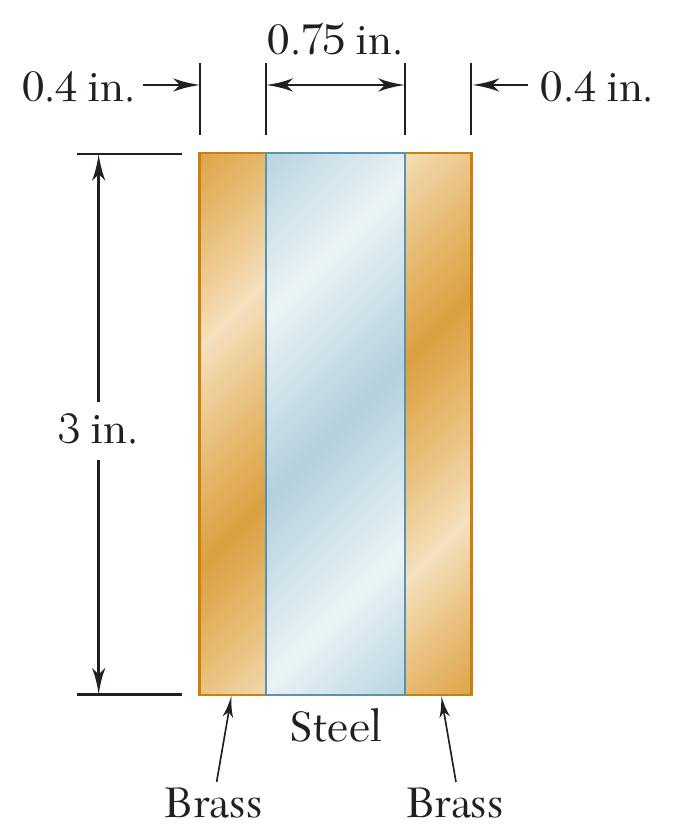
\includegraphics[width=\linewidth,height=4.7cm,keepaspectratio]{Chap_4/fig_4_24.png}
  \end{columns}
\end{frame}
% ===========
\section{Dầm bê tông cốt thép}
\begin{frame}[t]{Dầm bê tông cốt thép}
  \begin{columns}[T]
    \column{0.60\textwidth}
      \small
      \begin{itemize}
        \setlength{\itemsep}{0.5em}
        \item Dầm bê tông chịu mô men uốn được gia cường bằng các thanh
              cốt thép.
        \item Các thanh thép chịu toàn bộ lực kéo phía dưới mặt trung hòa.
              Phần trên của dầm bê tông chịu lực nén.
        \item Trong mặt cắt quy đổi, diện tích mặt cắt thép $A_s$ được thay
              bằng diện tích tương đương $nA_s$, với $n = E_s/E_c$.
        \item Để xác định vị trí trục trung hòa:
        \[
          (bx)\frac{x}{2} - nA_s(d - x) = 0
          \qquad
          \tfrac{1}{2}bx^2 + nA_sx - nA_sd = 0
        \]
        \item Ứng suất pháp trong bê tông và trong thép:
        \[
          \sigma_x = -\frac{My}{I} \qquad
          \sigma_c = \sigma_x \qquad \sigma_s = n\sigma_x
        \]
      \end{itemize}
    \column{0.38\textwidth}
      \centering
      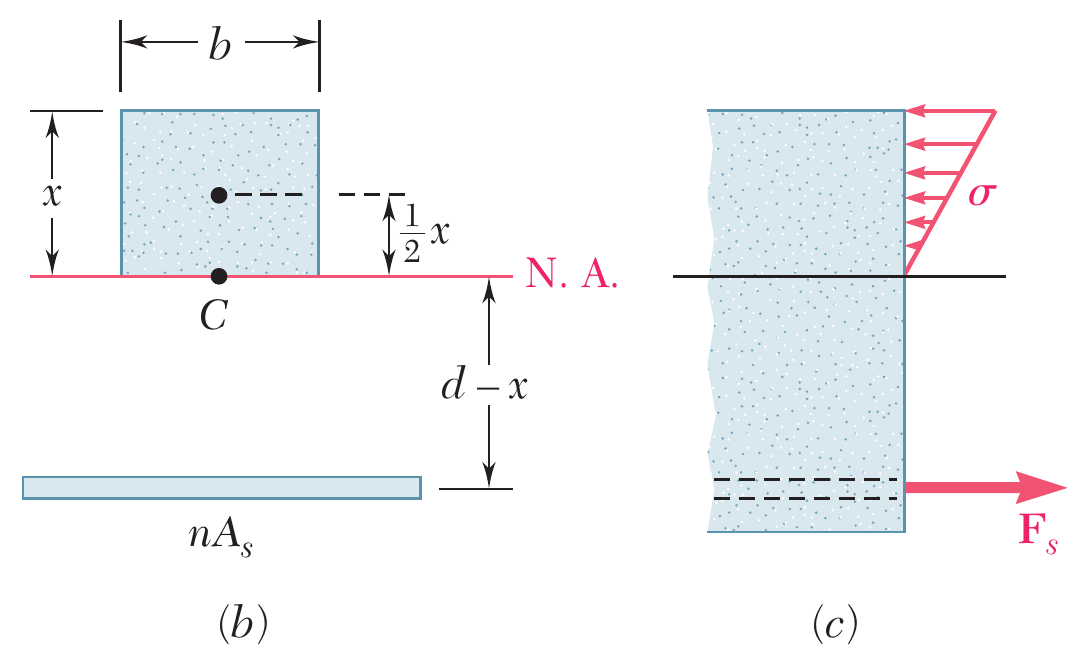
\includegraphics[width=\linewidth,height=5.5cm,keepaspectratio]{Chap_4/fig_4_26.png}
  \end{columns}
\end{frame}
% ===========
\section{Bài mẫu 4.4}
\begin{frame}[t]{Bài mẫu 4.4}
  \begin{columns}[T]
    \column{0.40\textwidth}
      \centering
      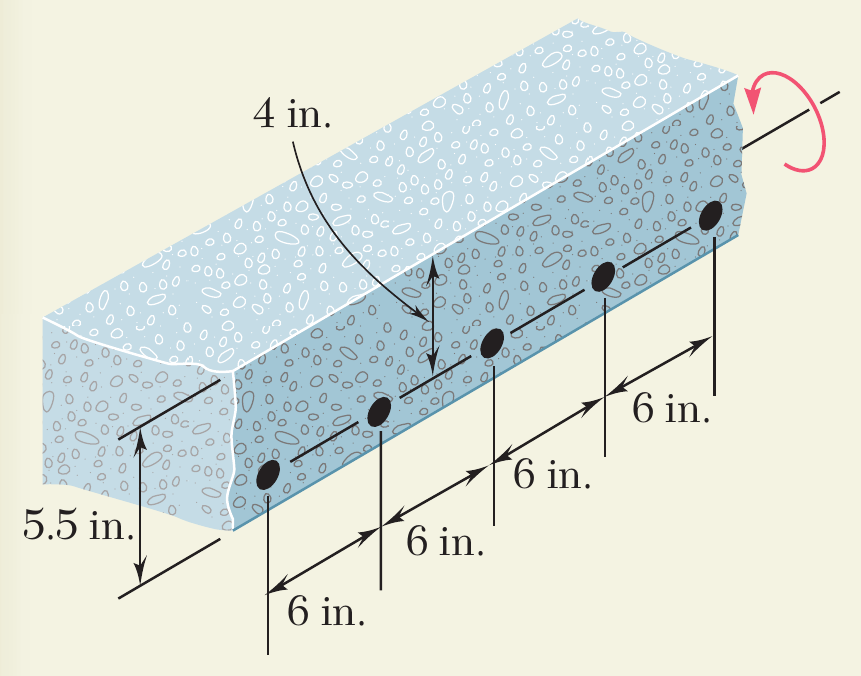
\includegraphics[width=\linewidth,height=5.5cm,keepaspectratio]{Chap_4/sp_4_4_a.png}
    \column{0.58\textwidth}
      \small
      Một sàn bê tông được gia cường bằng các thanh thép đường kính 16 mm.
      Mô đun đàn hồi của thép là 200 GPa và của bê tông là 25 GPa. Với mô
      men uốn $4{,}5\,\mathrm{kN\cdot m}$ trên mỗi 0,3 m bề rộng sàn, xác
      định ứng suất lớn nhất trong bê tông và trong thép.

      \vspace{0.8em}
      \textbf{LỜI GIẢI:}
      \begin{itemize}
        \setlength{\itemsep}{0.4em}
        \item Quy đổi thành mặt cắt hoàn toàn bằng bê tông.
        \item Tính các đặc trưng hình học của mặt cắt quy đổi.
        \item Tính ứng suất lớn nhất trong bê tông và trong thép.
      \end{itemize}
  \end{columns}
\end{frame}
% ===========
\begin{frame}[t]{Bài mẫu 4.4 (tiếp)}
  \begin{columns}[T]
    \column{0.60\textwidth}
      \small
      \textbf{LỜI GIẢI:}
      \begin{itemize}
        \setlength{\itemsep}{0.4em}
        \item Quy đổi thành mặt cắt hoàn toàn bằng bê tông:
        \[
          n = \frac{E_s}{E_c} = \frac{200\,\mathrm{GPa}}{25\,\mathrm{GPa}} = 8{,}0
          \qquad
          nA_s = 8{,}0\times2\left[\frac{\pi}{4}(16\,\mathrm{mm})^2\right]
        \]
        \item Tính các đặc trưng hình học của mặt cắt quy đổi:
        \[
          bx\frac{x}{2} - nA_s(d - x) = 0
          \quad\Rightarrow\quad x = 36{,}8\,\mathrm{mm}
        \]
        \[
          I = \tfrac{1}{3}bx^3 + nA_s(d - x)^2 = 12{,}8\times10^{-6}\,\mathrm{m}^4
        \]
        \item Tính các ứng suất lớn nhất:
        \[
          \sigma_c = \frac{Mc_1}{I}
            = \frac{4500\times0{,}0368}{12{,}8\times10^{-6}}
          \qquad \boxed{\sigma_c = 12{,}9\,\mathrm{MPa}}
        \]
        \[
          \sigma_s = n\frac{Mc_2}{I}
            = 8{,}0\,\frac{4500\times0{,}0632}{12{,}8\times10^{-6}}
          \qquad \boxed{\sigma_s = 177{,}8\,\mathrm{MPa}}
        \]
      \end{itemize}
    \column{0.38\textwidth}
      \centering
      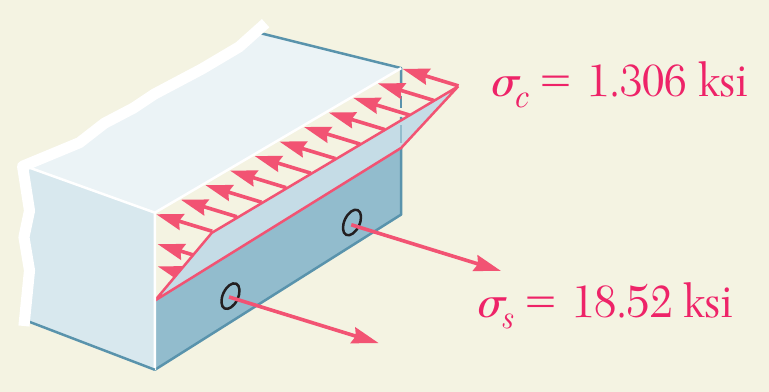
\includegraphics[width=\linewidth,height=2.9cm,keepaspectratio]{Chap_4/sp_4_4_b.png}\\[2pt]
      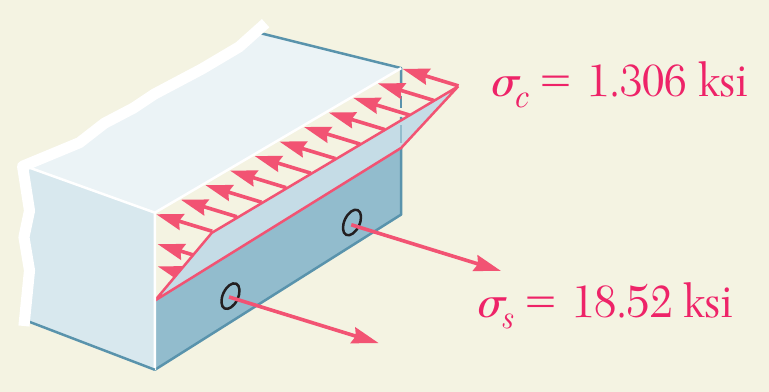
\includegraphics[width=\linewidth,height=2.9cm,keepaspectratio]{Chap_4/sp_4_4_b.png}
  \end{columns}
\end{frame}
% ===========
\section{Tập trung ứng suất}
\begin{frame}[t]{Tập trung ứng suất}
  \begin{columns}[T]
    \column{0.36\textwidth}
      \small
      Tập trung ứng suất có thể xuất hiện:
      \begin{itemize}
        \setlength{\itemsep}{0.5em}
        \item ở lân cận các điểm đặt tải trọng
        \item ở lân cận các vị trí mặt cắt ngang thay đổi đột ngột
      \end{itemize}
      \[
        \sigma_m = K\frac{Mc}{I}
      \]
    \column{0.62\textwidth}
      \centering
      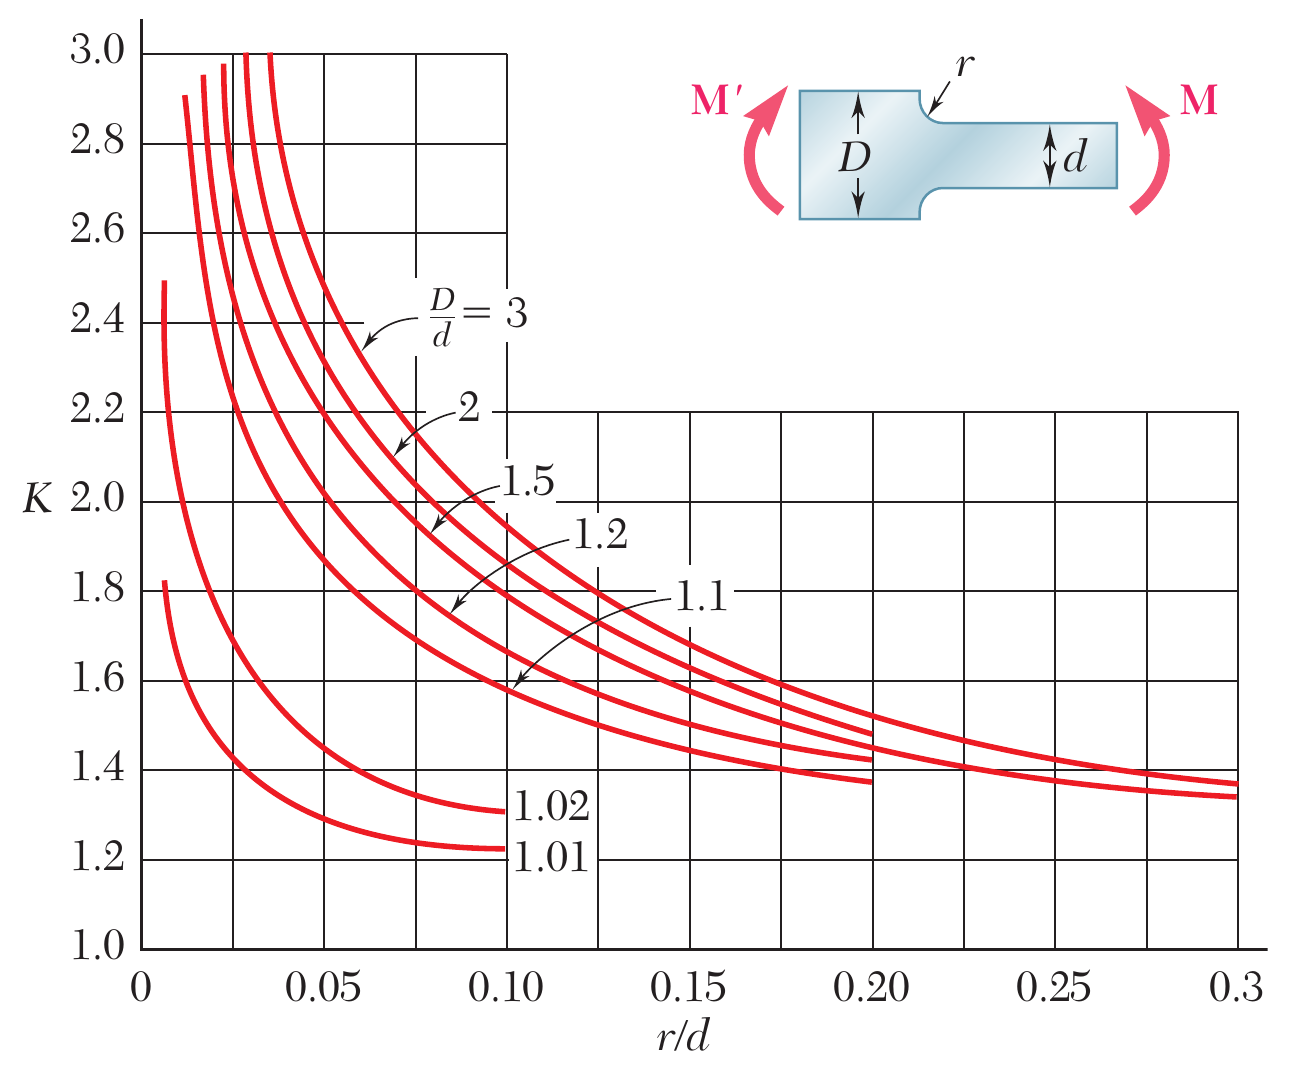
\includegraphics[width=0.49\linewidth,height=5.8cm,keepaspectratio]{Chap_4/fig_4_27.png}\hfill
      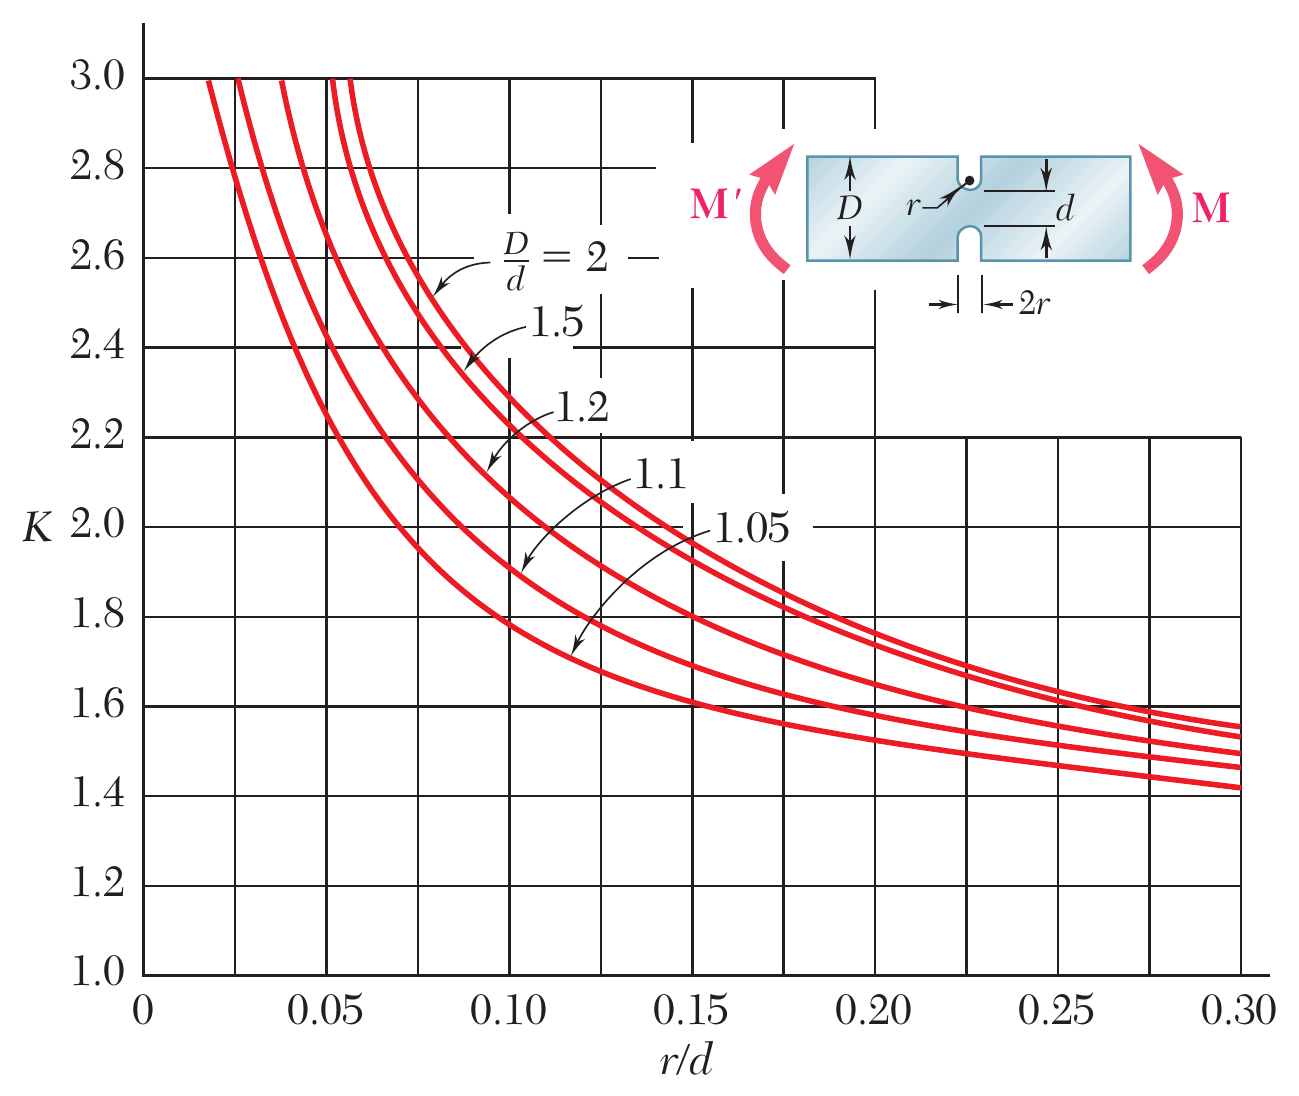
\includegraphics[width=0.49\linewidth,height=5.8cm,keepaspectratio]{Chap_4/fig_4_28.png}
  \end{columns}
\end{frame}
% ===========
\section{Biến dạng dẻo}
\begin{frame}[t]{Biến dạng dẻo}
  \begin{columns}[T]
    \column{0.60\textwidth}
      \footnotesize
      \begin{itemize}
        \setlength{\itemsep}{0.4em}
        \item Với mọi cấu kiện chịu uốn thuần túy:
        \[
          \varepsilon_x = -\frac{y}{c}\varepsilon_m
        \]
        (biến dạng thay đổi tuyến tính theo chiều cao mặt cắt)
        \item Nếu cấu kiện làm bằng vật liệu đàn hồi tuyến tính, trục trung
              hòa đi qua trọng tâm mặt cắt và
              $\displaystyle \sigma_x = -\frac{My}{I}$.
        \item Với vật liệu có đường cong ứng suất -- biến dạng phi tuyến, vị
              trí trục trung hòa được xác định từ điều kiện:
        \[
          F_x = \int\sigma_x\,dA = 0 \qquad M = \int -y\sigma_x\,dA
        \]
        \item Với cấu kiện có mặt phẳng đối xứng đứng và ngang, và vật liệu
              có quan hệ ứng suất -- biến dạng khi kéo và nén như nhau, trục
              trung hòa nằm tại trọng tâm mặt cắt và quan hệ ứng suất --
              biến dạng có thể dùng để chuyển phân bố biến dạng thành phân
              bố ứng suất.
      \end{itemize}
    \column{0.38\textwidth}
      \centering
      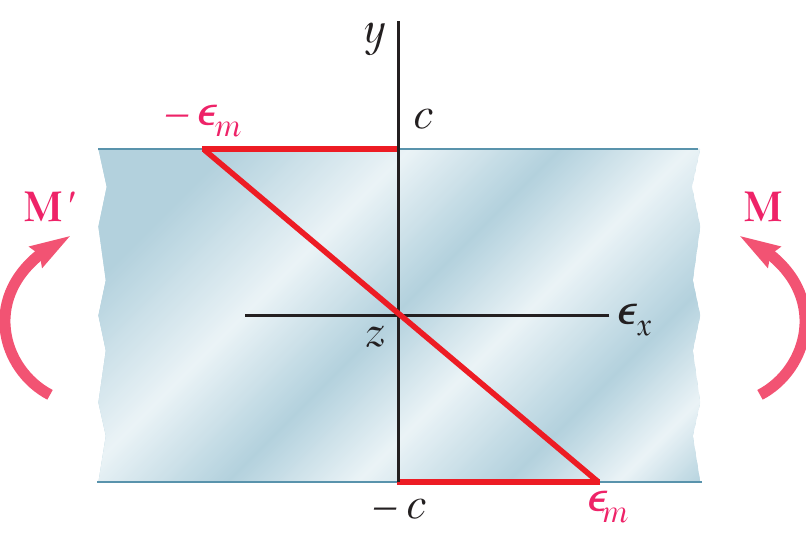
\includegraphics[width=\linewidth,height=1.9cm,keepaspectratio]{Chap_4/fig_4_30.png}\\[2pt]
      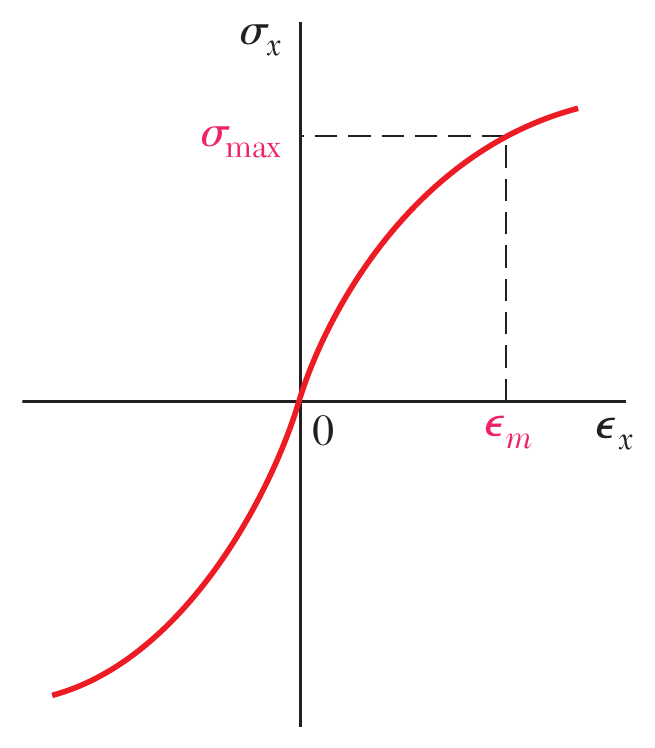
\includegraphics[width=\linewidth,height=1.9cm,keepaspectratio]{Chap_4/fig_4_31.png}\\[2pt]
      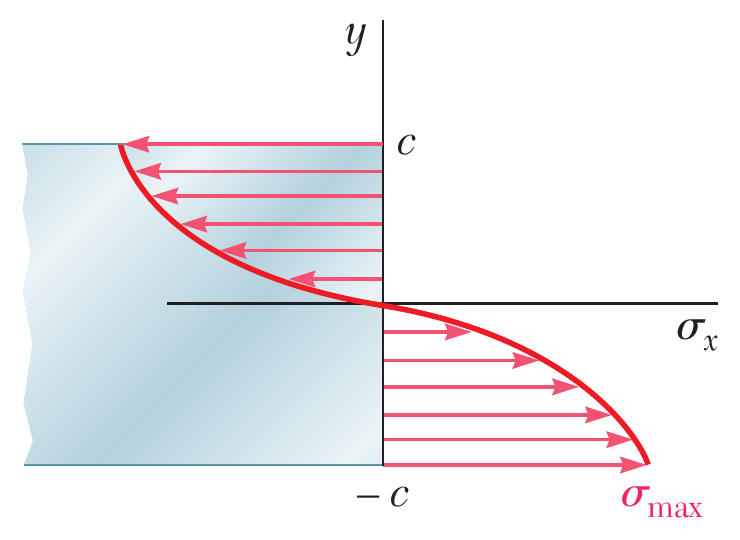
\includegraphics[width=\linewidth,height=1.9cm,keepaspectratio]{Chap_4/fig_4_32.png}
  \end{columns}
\end{frame}
% ===========
\begin{frame}[t]{Biến dạng dẻo (tiếp)}
  \begin{columns}[T]
    \column{0.58\textwidth}
      \small
      \begin{itemize}
        \setlength{\itemsep}{0.7em}
        \item Khi ứng suất lớn nhất bằng giới hạn bền của vật liệu, phá hủy
              xảy ra và mô men tương ứng $M_U$ được gọi là \emph{mô men uốn
              giới hạn}.
        \item \emph{Mô đun phá hủy khi uốn} $R_B$ được xác định từ giá trị
              $M_U$ đo bằng thực nghiệm và một phân bố ứng suất tuyến tính
              giả định:
        \[
          R_B = \frac{M_Uc}{I}
        \]
        \item $R_B$ có thể dùng để xác định $M_U$ của mọi cấu kiện làm cùng
              vật liệu và có cùng hình dạng mặt cắt nhưng kích thước khác.
      \end{itemize}
    \column{0.40\textwidth}
      \centering
      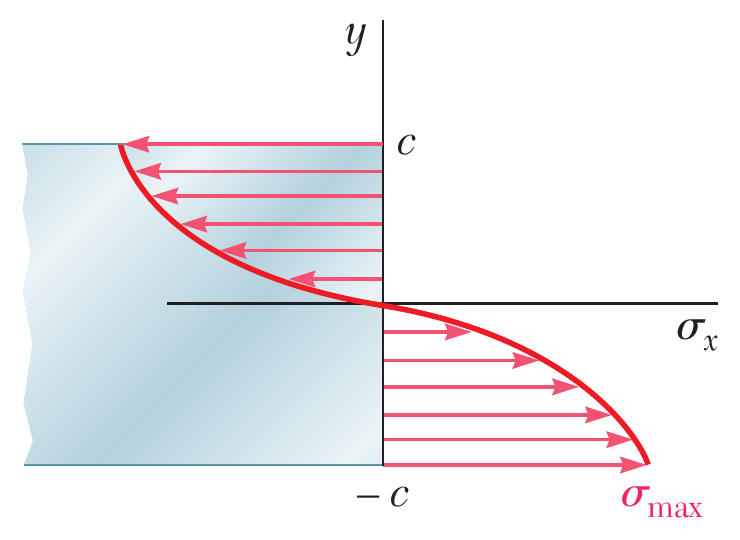
\includegraphics[width=\linewidth,height=2.9cm,keepaspectratio]{Chap_4/fig_4_32.png}\\[2pt]
      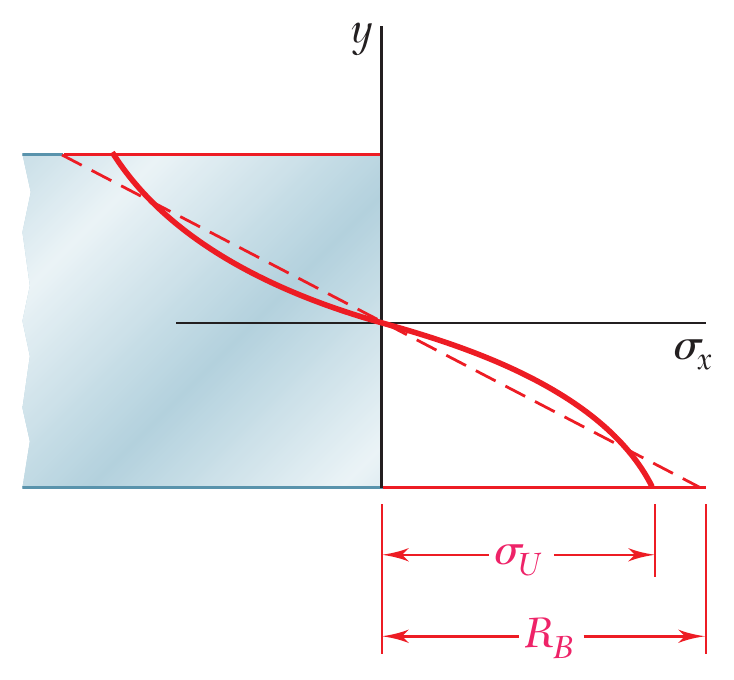
\includegraphics[width=\linewidth,height=2.9cm,keepaspectratio]{Chap_4/fig_4_33.png}
  \end{columns}
\end{frame}
% ===========
\section{Cấu kiện làm bằng vật liệu đàn -- dẻo}
\begin{frame}[t]{Cấu kiện làm bằng vật liệu đàn -- dẻo}
  \begin{columns}[T]
    \column{0.62\textwidth}
      \footnotesize
      \begin{itemize}
        \setlength{\itemsep}{0.35em}
        \item Dầm chữ nhật làm bằng vật liệu đàn -- dẻo:
        \[
          \sigma_x \le \sigma_Y \qquad \sigma_m = \frac{Mc}{I}
        \]
        \[
          \sigma_m = \sigma_Y \qquad
          M_Y = \frac{I}{c}\sigma_Y = \text{mô men đàn hồi lớn nhất}
        \]
        \item Nếu mô men tăng vượt quá mô men đàn hồi lớn nhất, các vùng
              dẻo hình thành bao quanh một lõi đàn hồi:
        \[
          M = \tfrac{3}{2}M_Y\left(1 - \tfrac{1}{3}\frac{y_Y^2}{c^2}\right)
          \qquad y_Y = \text{nửa chiều dày lõi đàn hồi}
        \]
        \item Khi mô men tiếp tục tăng, chiều dày lõi đàn hồi tiến về
              không, tương ứng với trạng thái chảy dẻo hoàn toàn:
        \[
          M_p = \tfrac{3}{2}M_Y = \text{mô men dẻo}
        \]
        \[
          k = \frac{M_p}{M_Y} = \text{hệ số hình dạng
            (chỉ phụ thuộc hình dạng mặt cắt)}
        \]
      \end{itemize}
    \column{0.36\textwidth}
      \centering
      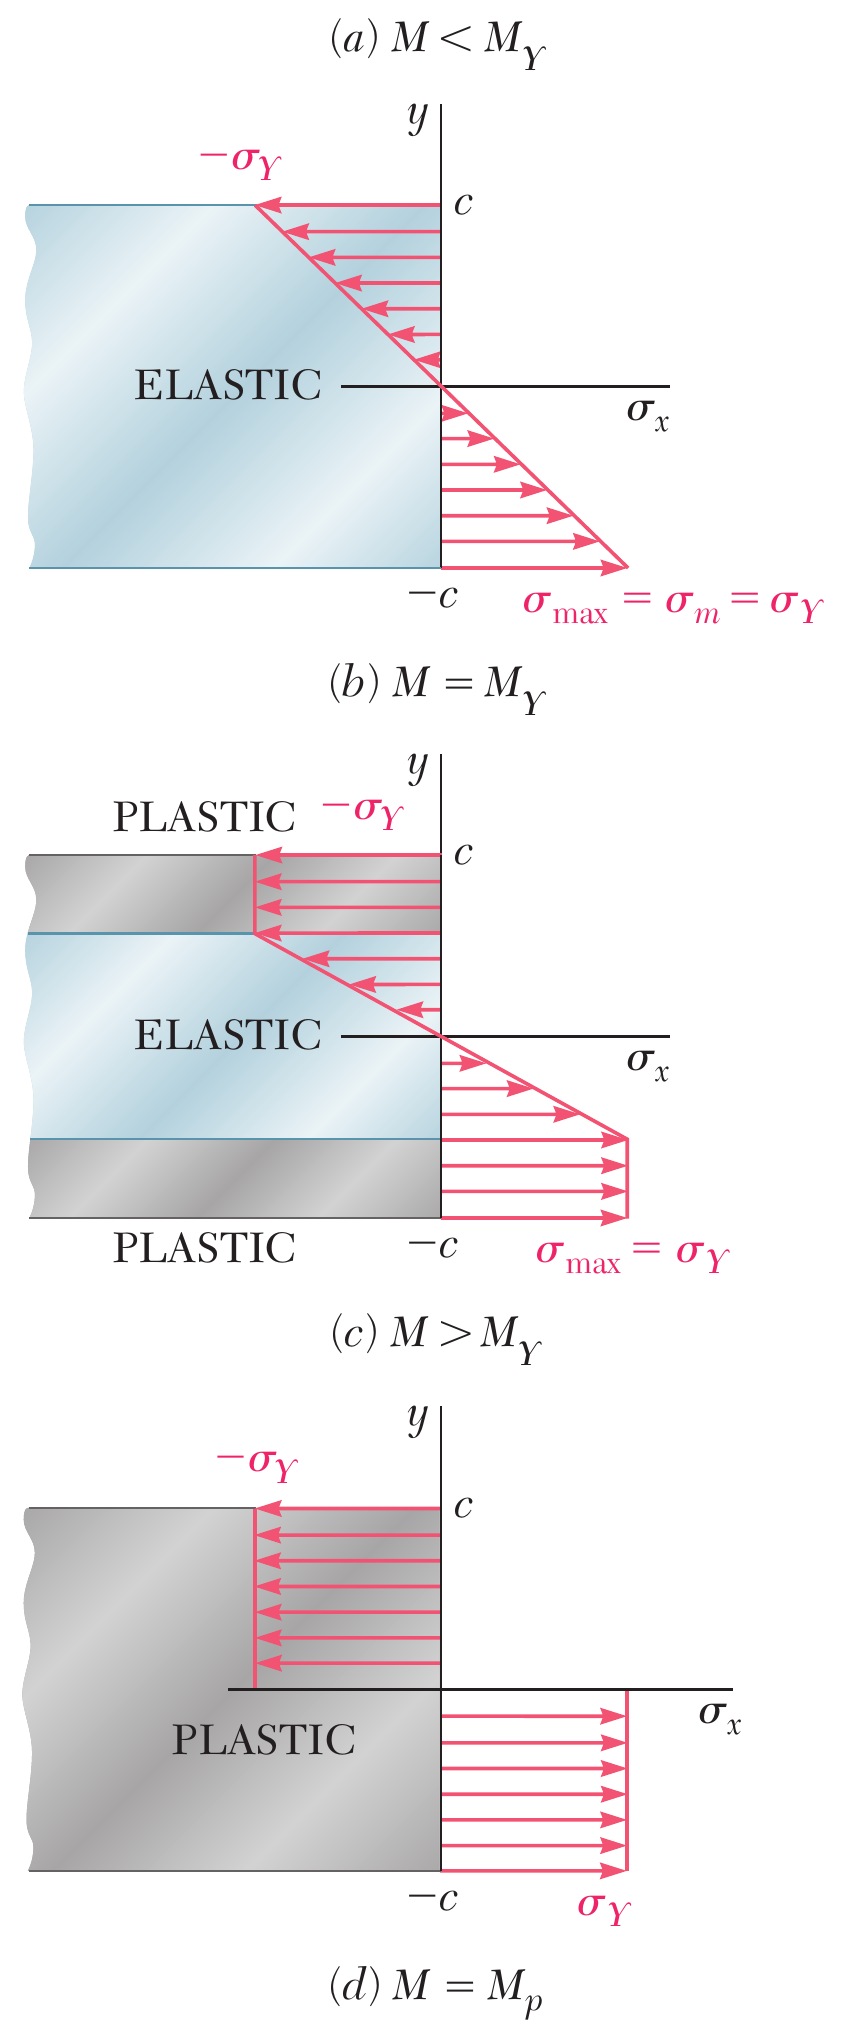
\includegraphics[width=\linewidth,height=5.5cm,keepaspectratio]{Chap_4/fig_4_36.png}
  \end{columns}
\end{frame}
% ===========
\section{Biến dạng dẻo của cấu kiện có một mặt phẳng đối xứng}
\begin{frame}[t]{Biến dạng dẻo của cấu kiện có một mặt phẳng đối xứng}
  \begin{columns}[T]
    \column{0.58\textwidth}
      \small
      \begin{itemize}
        \setlength{\itemsep}{0.6em}
        \item Biến dạng dẻo hoàn toàn của dầm chỉ có một mặt phẳng đối
              xứng đứng.
        \item Không thể giả thiết trục trung hòa đi qua trọng tâm mặt cắt.
        \item Hợp lực $R_1$ và $R_2$ của các lực nén và kéo phân tố tạo
              thành một ngẫu lực:
        \[
          R_1 = R_2 \qquad A_1\sigma_Y = A_2\sigma_Y
        \]
        Trục trung hòa chia mặt cắt thành hai phần có diện tích bằng nhau.
        \item Mô men dẻo của cấu kiện:
        \[
          M_p = \left(\tfrac{1}{2}A\sigma_Y\right)d
        \]
      \end{itemize}
    \column{0.40\textwidth}
      \centering
      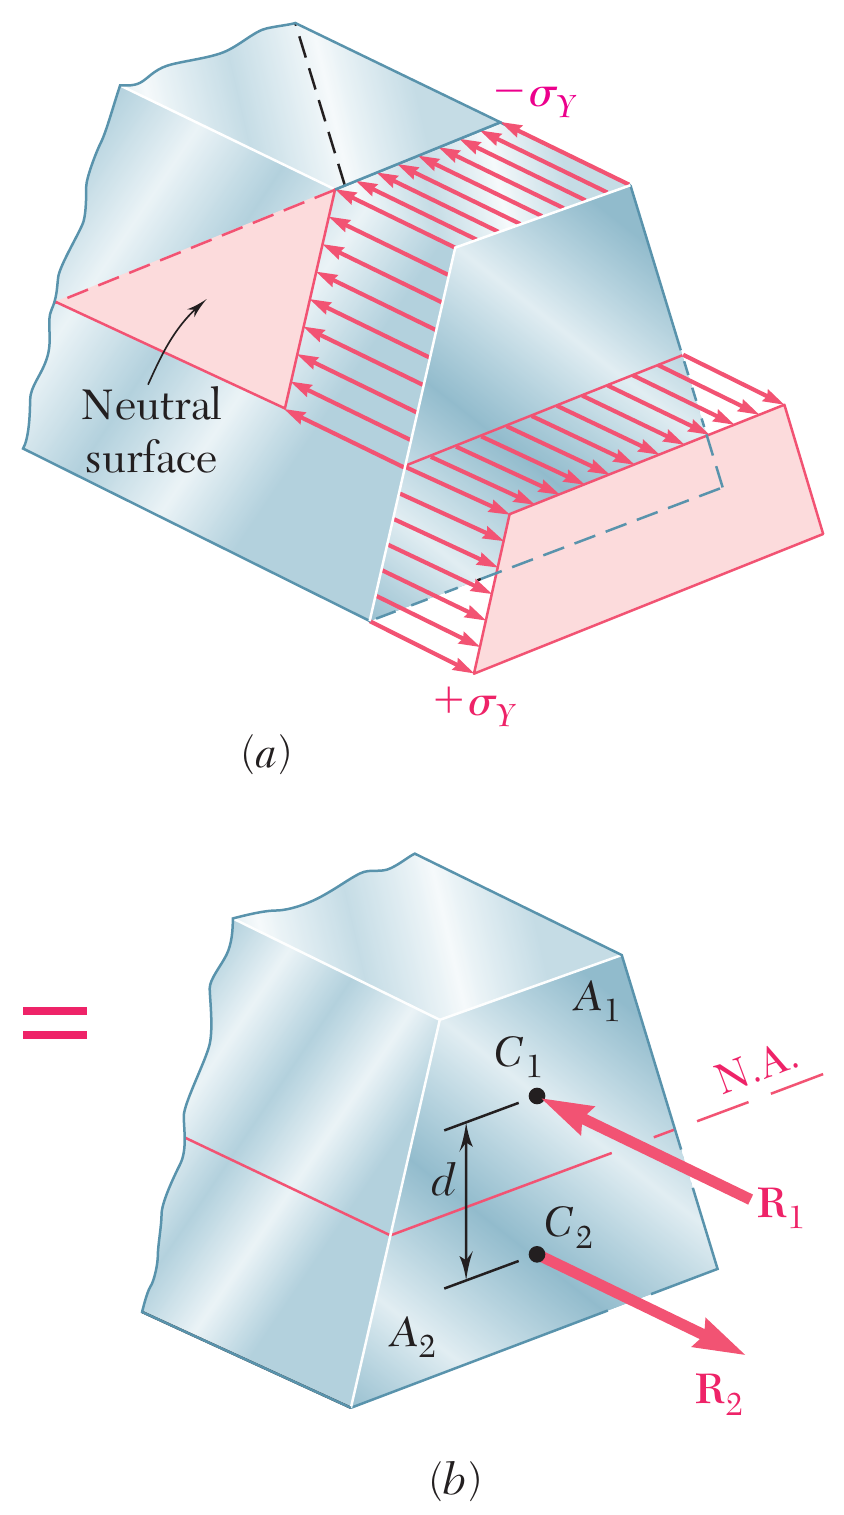
\includegraphics[width=\linewidth,height=5.5cm,keepaspectratio]{Chap_4/fig_4_39.png}
  \end{columns}
\end{frame}
% ===========
\section{Ứng suất dư}
\begin{frame}[t]{Ứng suất dư}
  \begin{columns}[T]
    \column{0.58\textwidth}
      \small
      \begin{itemize}
        \setlength{\itemsep}{0.6em}
        \item Các vùng dẻo hình thành trong cấu kiện làm bằng vật liệu đàn
              -- dẻo nếu mô men uốn đủ lớn.
        \item Vì quan hệ tuyến tính giữa ứng suất pháp và biến dạng đúng tại
              mọi điểm trong giai đoạn dỡ tải, có thể xử lý giai đoạn này
              bằng cách coi cấu kiện là hoàn toàn đàn hồi.
        \item Ứng suất dư nhận được bằng cách áp dụng nguyên lý cộng tác
              dụng: tổ hợp ứng suất khi chất tải với mô men $M$ (biến dạng
              đàn -- dẻo) và khi dỡ tải với mô men $-M$ (biến dạng đàn hồi).
        \item Giá trị cuối cùng của ứng suất tại một điểm nói chung khác
              không.
      \end{itemize}
    \column{0.40\textwidth}
      \centering
      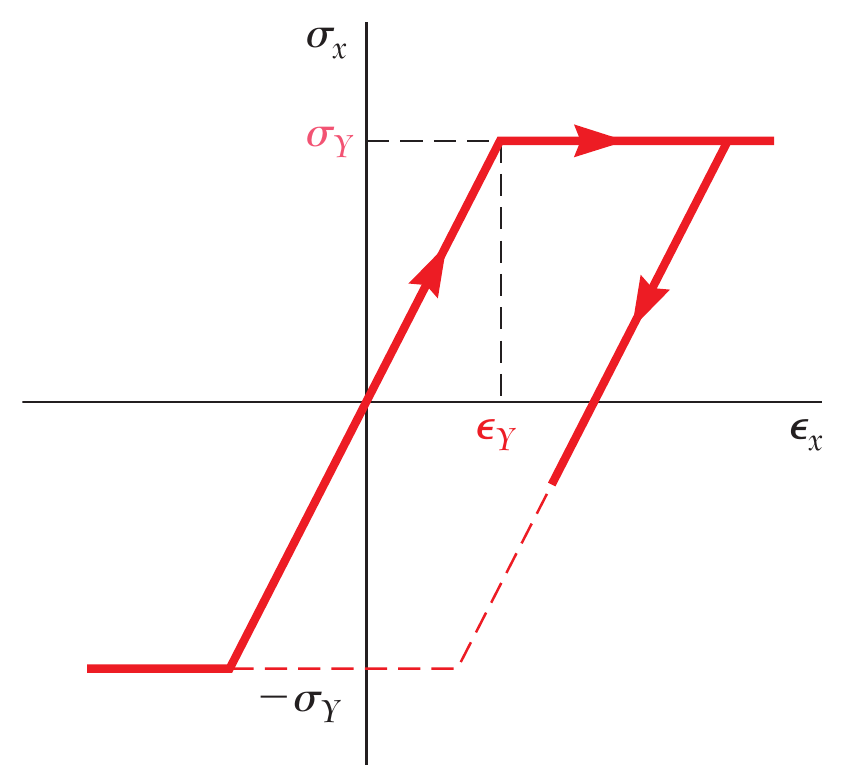
\includegraphics[width=\linewidth,height=5.5cm,keepaspectratio]{Chap_4/fig_4_40.png}
  \end{columns}
\end{frame}
% ===========
\section{Ví dụ 4.05, 4.06}
\begin{frame}[t]{Ví dụ 4.05, 4.06}
  \begin{columns}[T]
    \column{0.40\textwidth}
      \centering
      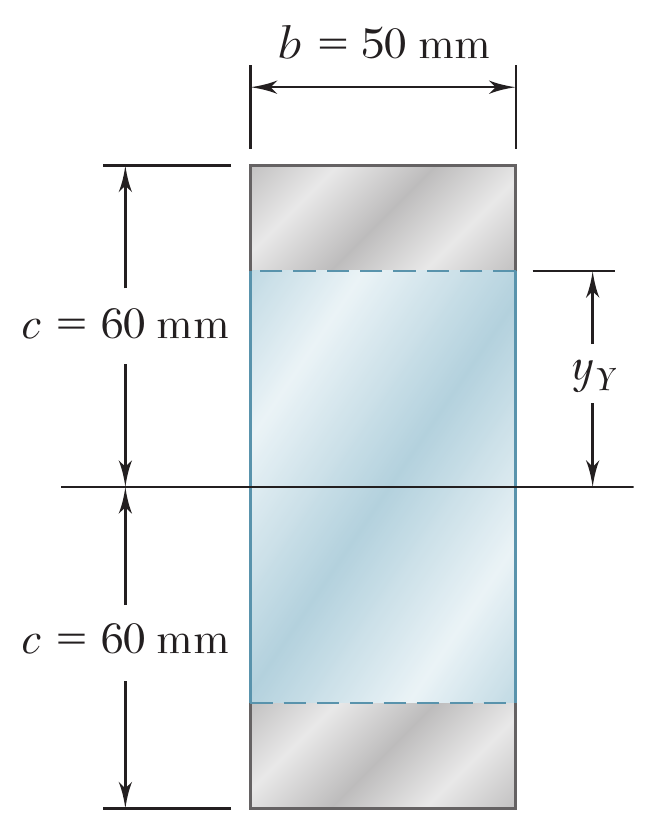
\includegraphics[width=\linewidth,height=5.5cm,keepaspectratio]{Chap_4/fig_4_38.png}
    \column{0.58\textwidth}
      \small
      Một cấu kiện có mặt cắt chữ nhật không đổi chịu mô men uốn
      $M = 36{,}8\,\mathrm{kN\cdot m}$. Cấu kiện làm bằng vật liệu đàn --
      dẻo có giới hạn chảy 240 MPa và mô đun đàn hồi 200 GPa.

      \vspace{0.5em}
      Xác định (a) chiều dày lõi đàn hồi, (b) bán kính cong của mặt trung
      hòa.

      \vspace{0.5em}
      Sau khi tải trọng giảm về không, xác định (c) phân bố ứng suất dư,
      (d) bán kính cong.
  \end{columns}
\end{frame}
% ===========
\begin{frame}[t]{Ví dụ 4.05, 4.06 (tiếp)}
  \begin{columns}[T]
    \column{0.62\textwidth}
      \footnotesize
      \begin{itemize}
        \setlength{\itemsep}{0.3em}
        \item Mô men đàn hồi lớn nhất:
        \[
          \frac{I}{c} = \tfrac{2}{3}bc^2
            = \tfrac{2}{3}(50\times10^{-3}\,\mathrm{m})(60\times10^{-3}\,\mathrm{m})^2
            = 120\times10^{-6}\,\mathrm{m}^3
        \]
        \[
          M_Y = \frac{I}{c}\sigma_Y = (120\times10^{-6}\,\mathrm{m}^3)(240\,\mathrm{MPa})
            = 28{,}8\,\mathrm{kN\cdot m}
        \]
        \item Chiều dày lõi đàn hồi:
        \[
          M = \tfrac{3}{2}M_Y\left(1 - \tfrac{1}{3}\frac{y_Y^2}{c^2}\right)
          \quad\Rightarrow\quad
          36{,}8 = \tfrac{3}{2}(28{,}8)\left(1 - \tfrac{1}{3}\frac{y_Y^2}{c^2}\right)
        \]
        \[
          \frac{y_Y}{c} = 0{,}666 \qquad \boxed{2y_Y = 80\,\mathrm{mm}}
        \]
        \item Bán kính cong:
        \[
          \varepsilon_Y = \frac{\sigma_Y}{E} = \frac{240\times10^{6}\,\mathrm{Pa}}{200\times10^{9}\,\mathrm{Pa}}
            = 1{,}2\times10^{-3}
        \]
        \[
          \varepsilon_Y = \frac{y_Y}{\rho}
          \quad\Rightarrow\quad
          \rho = \frac{y_Y}{\varepsilon_Y} = \frac{40\times10^{-3}\,\mathrm{m}}{1{,}2\times10^{-3}}
          \qquad \boxed{\rho = 33{,}3\,\mathrm{m}}
        \]
      \end{itemize}
    \column{0.36\textwidth}
      \centering
      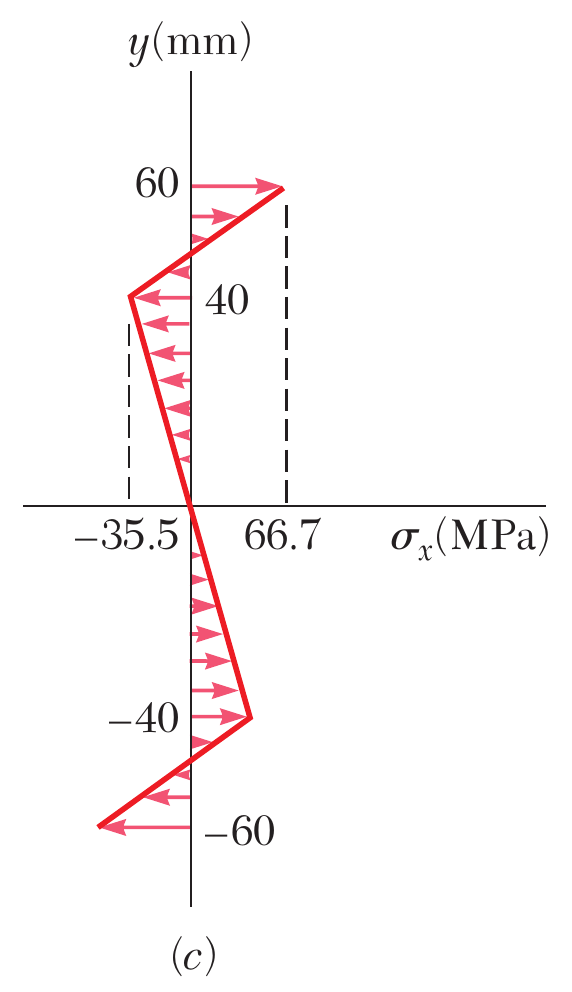
\includegraphics[width=\linewidth,height=5.5cm,keepaspectratio]{Chap_4/ex_4_06.png}
  \end{columns}
\end{frame}
% ===========
\begin{frame}[t]{Ví dụ 4.05, 4.06 (tiếp)}
  \begin{columns}[T]
    \column{0.52\textwidth}
      \small
      \begin{itemize}
        \setlength{\itemsep}{0.5em}
        \item $M = 36{,}8\,\mathrm{kN\cdot m}$:
              $y_Y = 40\,\mathrm{mm}$, $\sigma_Y = 240\,\mathrm{MPa}$
        \item $M = -36{,}8\,\mathrm{kN\cdot m}$:
        \[
          \sigma'_m = \frac{Mc}{I} = \frac{36{,}8\,\mathrm{kN\cdot m}}{120\times10^{-6}\,\mathrm{m}^3}
            = 306{,}7\,\mathrm{MPa} < 2\sigma_Y
        \]
        \item $M = 0$: Tại biên của lõi đàn hồi,
        \[
          \varepsilon_x = \frac{\sigma_x}{E} = \frac{-35{,}5\times10^{6}\,\mathrm{Pa}}{200\times10^{9}\,\mathrm{Pa}}
            = -177{,}5\times10^{-6}
        \]
        \[
          \rho = -\frac{y_Y}{\varepsilon_x} = \frac{40\times10^{-3}\,\mathrm{m}}{177{,}5\times10^{-6}}
          \qquad \boxed{\rho = 225\,\mathrm{m}}
        \]
      \end{itemize}
    \column{0.46\textwidth}
      \centering
      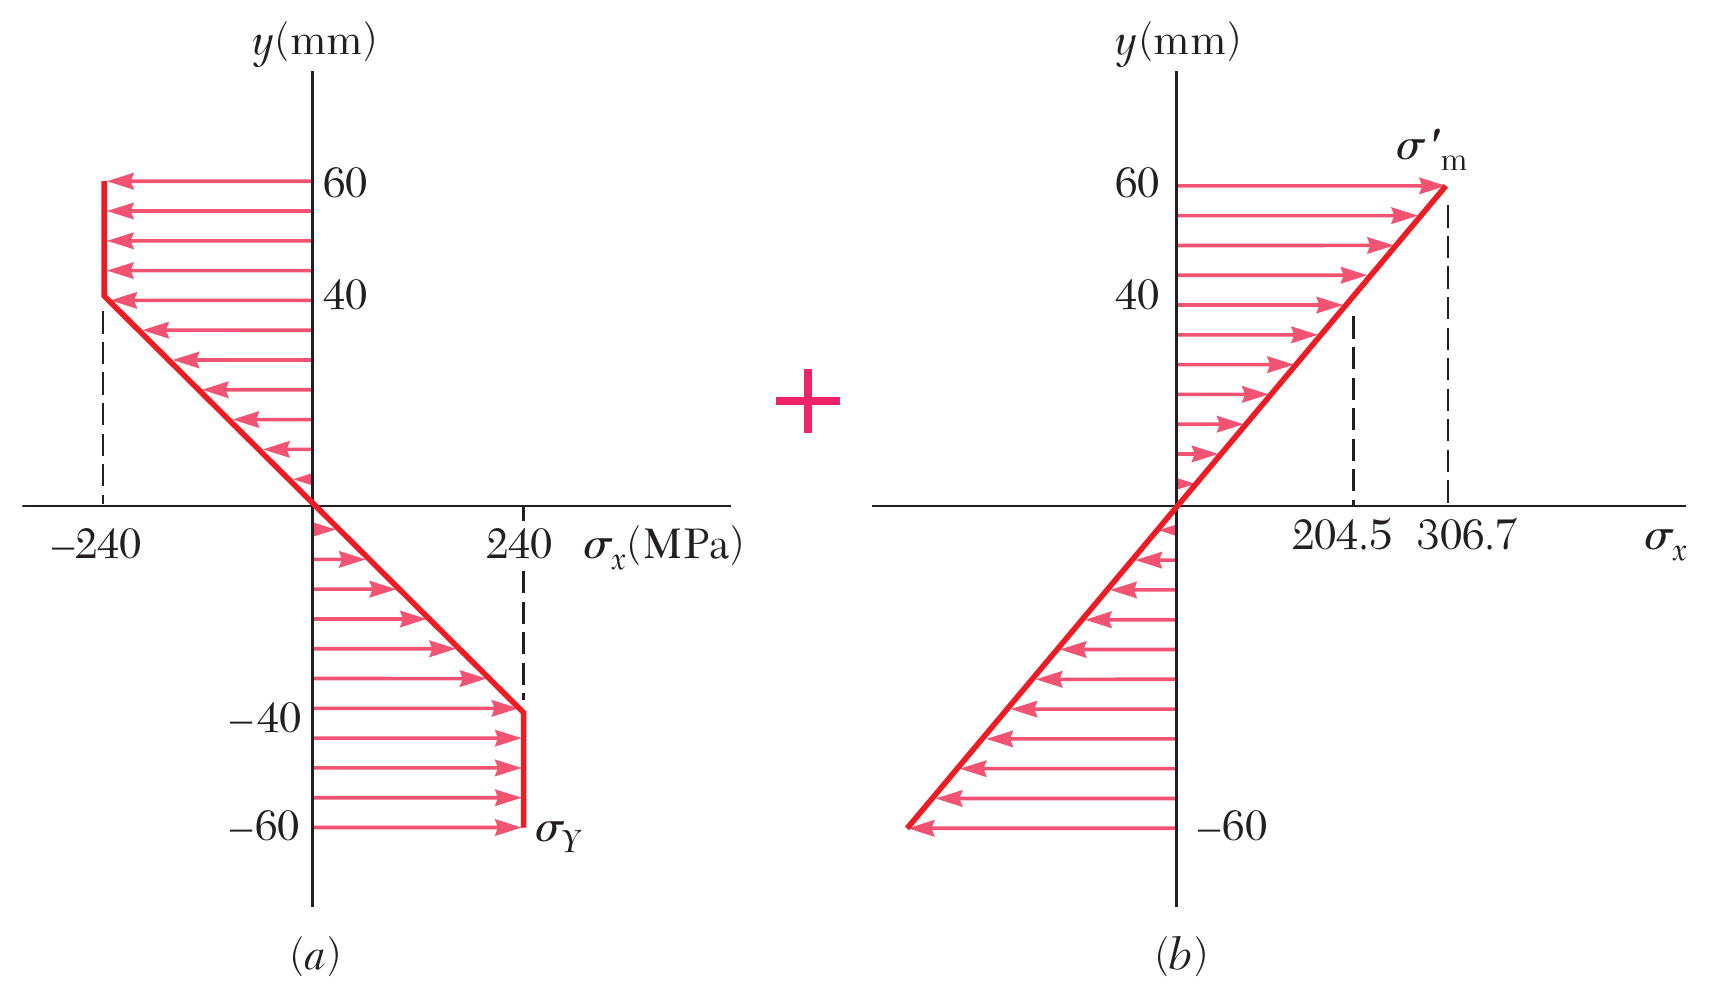
\includegraphics[width=0.49\linewidth,height=2.9cm,keepaspectratio]{Chap_4/fig_4_41.png}\hfill
      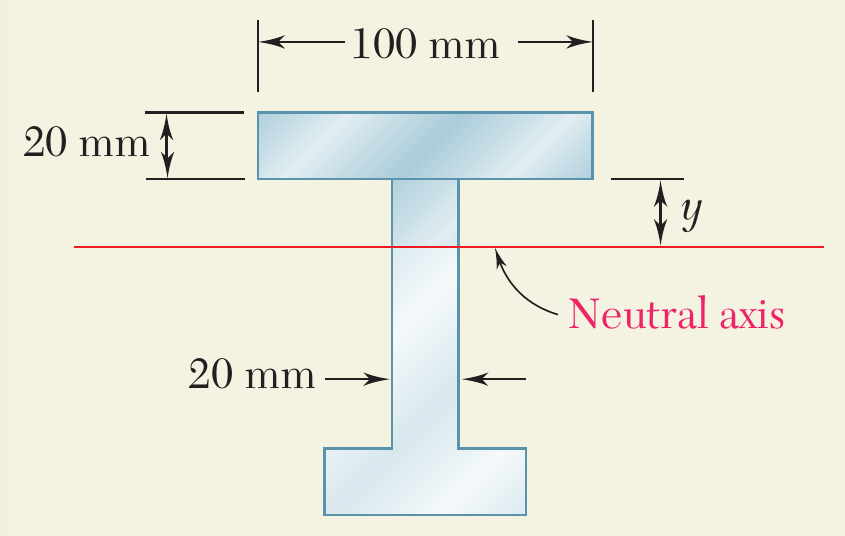
\includegraphics[width=0.49\linewidth,height=2.9cm,keepaspectratio]{Chap_4/sp_4_6_a.png}\\[2pt]
      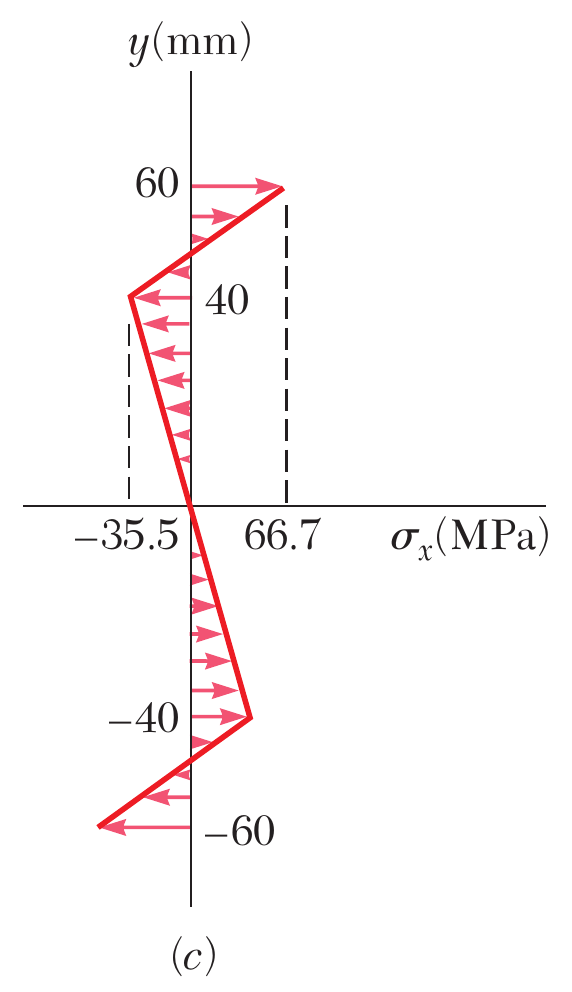
\includegraphics[width=0.49\linewidth,height=2.9cm,keepaspectratio]{Chap_4/ex_4_06.png}\hfill
      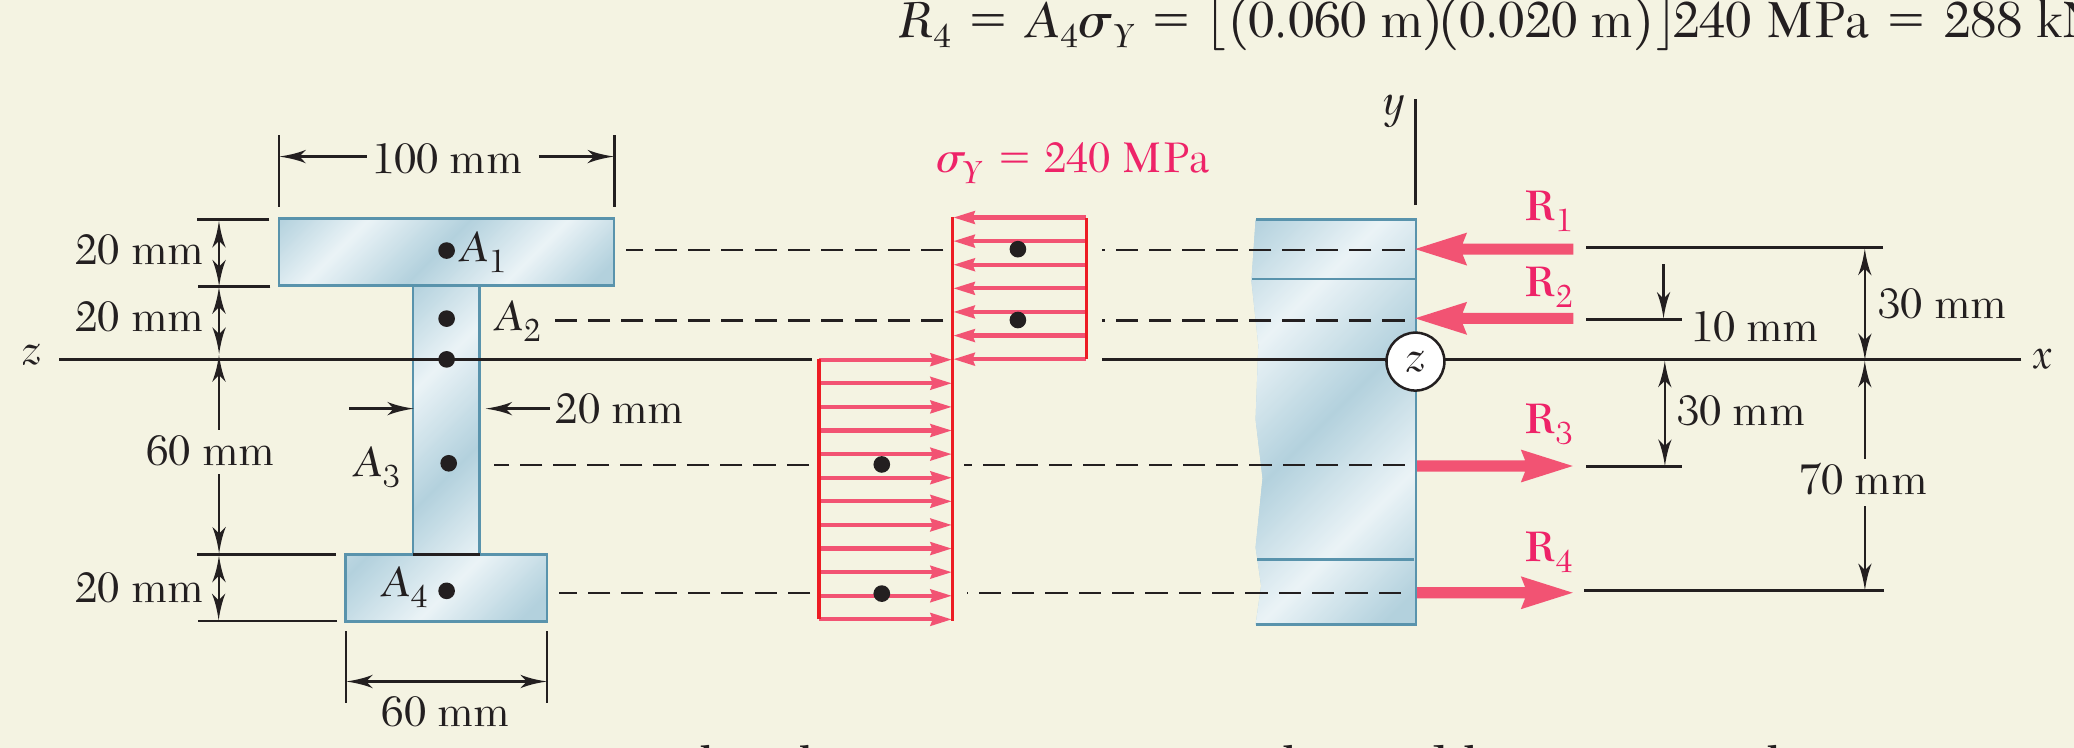
\includegraphics[width=0.49\linewidth,height=2.9cm,keepaspectratio]{Chap_4/sp_4_6_b.png}
  \end{columns}
\end{frame}
% ===========
\section{Tải trọng dọc trục lệch tâm trong mặt phẳng đối xứng}
\begin{frame}[t]{Tải trọng dọc trục lệch tâm trong mặt phẳng đối xứng}
  \begin{columns}[T]
    \column{0.58\textwidth}
      \small
      \begin{itemize}
        \setlength{\itemsep}{0.6em}
        \item Ứng suất do tải trọng lệch tâm được xác định bằng cách cộng
              tác dụng ứng suất phân bố đều do lực đúng tâm và ứng suất
              phân bố tuyến tính do mô men uốn thuần túy:
        \[
          \sigma_x = (\sigma_x)_{\text{đúng tâm}} + (\sigma_x)_{\text{uốn}}
                   = \frac{P}{A} - \frac{My}{I}
        \]
        \item Tải trọng lệch tâm:
        \[
          F = P \qquad M = Pd
        \]
        \item Điều kiện áp dụng: ứng suất nhỏ hơn giới hạn tỉ lệ, biến dạng
              ảnh hưởng không đáng kể đến hình học, và ứng suất không được
              tính ở gần điểm đặt lực.
      \end{itemize}
    \column{0.40\textwidth}
      \centering
      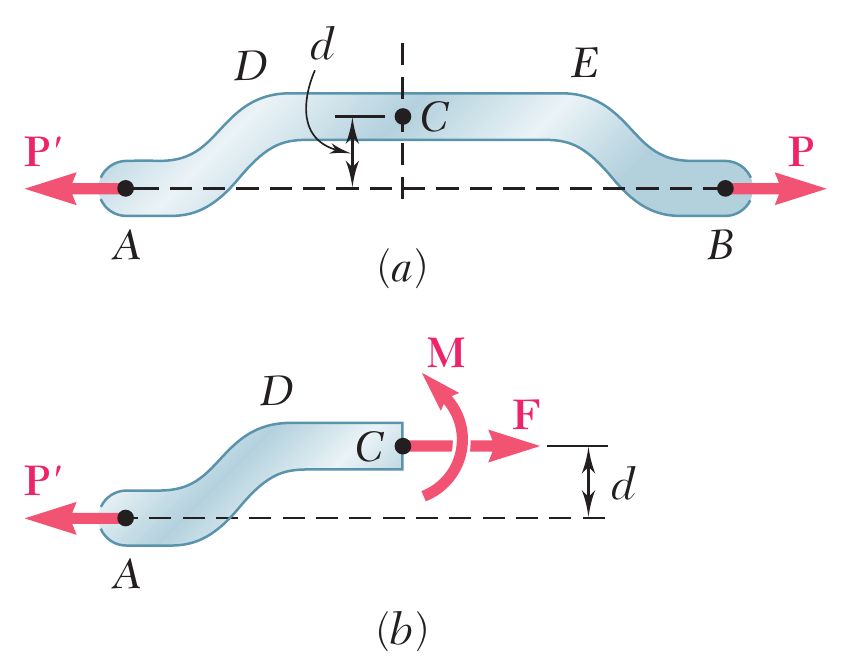
\includegraphics[width=\linewidth,height=2.9cm,keepaspectratio]{Chap_4/fig_4_42.png}\\[2pt]
      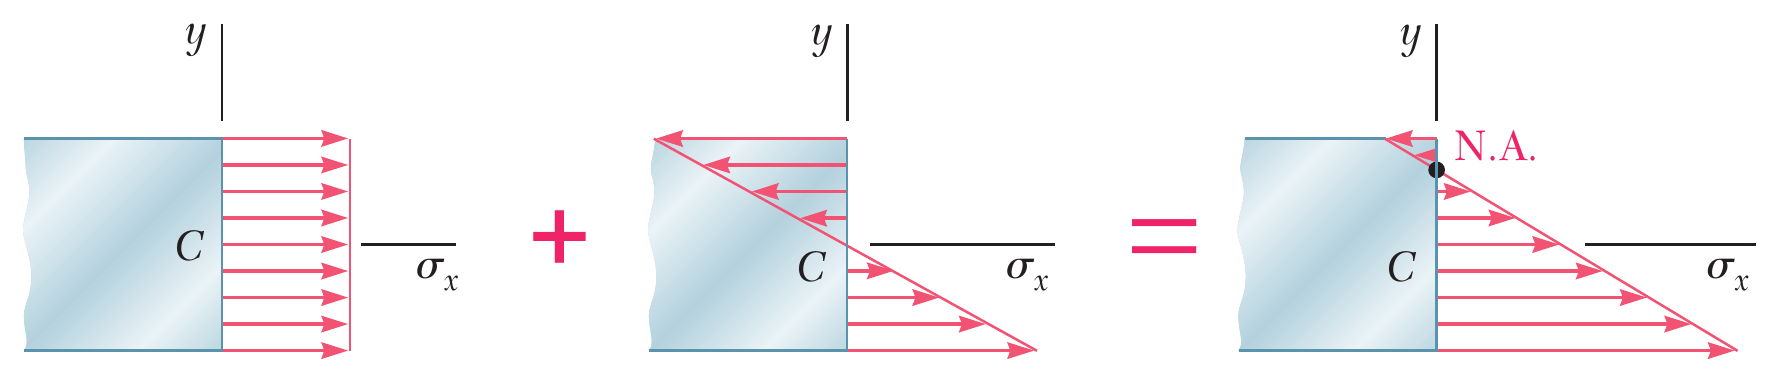
\includegraphics[width=\linewidth,height=2.9cm,keepaspectratio]{Chap_4/fig_4_45.png}
  \end{columns}
\end{frame}
% ===========
\section{Ví dụ 4.07}
\begin{frame}[t]{Ví dụ 4.07}
  \begin{columns}[T]
    \column{0.40\textwidth}
      \centering
      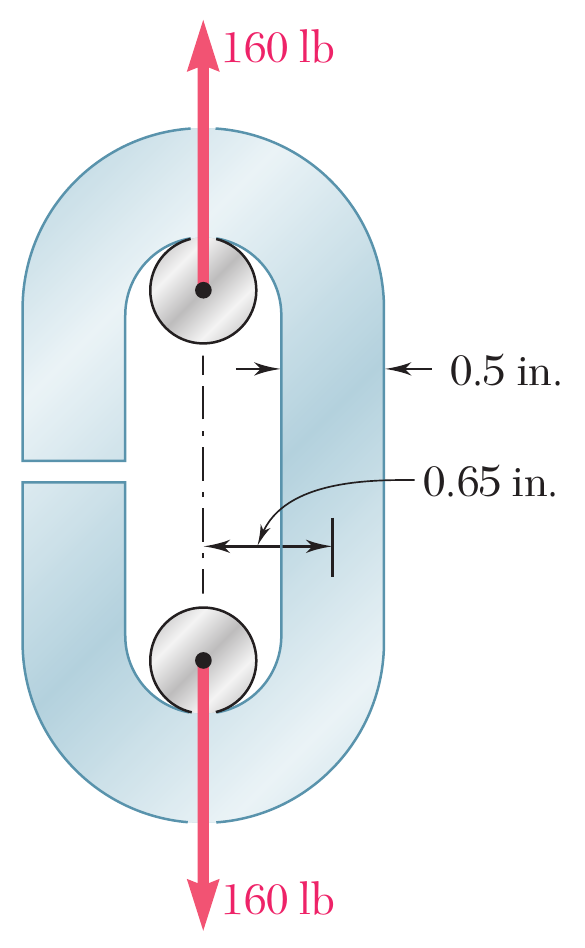
\includegraphics[width=\linewidth,height=5.5cm,keepaspectratio]{Chap_4/fig_4_46.png}
    \column{0.58\textwidth}
      \small
      Một mắt xích hở được tạo bằng cách uốn các thanh thép cacbon thấp
      thành hình dạng như hình vẽ. Với tải trọng 700 N, xác định (a) ứng
      suất kéo và nén lớn nhất, (b) khoảng cách giữa trọng tâm mặt cắt và
      trục trung hòa.

      \vspace{0.5em}
      \textbf{LỜI GIẢI:}
      \begin{itemize}
        \setlength{\itemsep}{0.3em}
        \item Tìm lực đúng tâm và mô men uốn tương đương.
        \item Cộng tác dụng ứng suất phân bố đều do lực đúng tâm và ứng suất
              tuyến tính do mô men uốn.
        \item Tính ứng suất kéo và nén lớn nhất tại mép trong và mép ngoài
              của phân bố ứng suất tổng hợp.
        \item Tìm trục trung hòa bằng cách xác định vị trí có ứng suất pháp
              bằng không.
      \end{itemize}
  \end{columns}
\end{frame}
% ===========
\begin{frame}[t]{Ví dụ 4.07 (tiếp)}
  \begin{columns}[T]
    \column{0.49\textwidth}
      \small
      \begin{itemize}
        \setlength{\itemsep}{0.4em}
        \item Lực đúng tâm và mô men uốn tương đương:
        \[
          P = 700\,\mathrm{N}
        \]
        \[
          M = Pd = (700\,\mathrm{N})(0{,}016\,\mathrm{m}) = 11{,}2\,\mathrm{N\cdot m}
        \]
        \item Ứng suất pháp do lực đúng tâm:
        \[
          A = \pi c^2 = \pi(6\,\mathrm{mm})^2 = 113{,}1\,\mathrm{mm}^2
        \]
        \[
          \sigma_0 = \frac{P}{A} = \frac{700\,\mathrm{N}}{113{,}1\times10^{-6}\,\mathrm{m}^2}
            = 6{,}2\,\mathrm{MPa}
        \]
      \end{itemize}
      \centering
      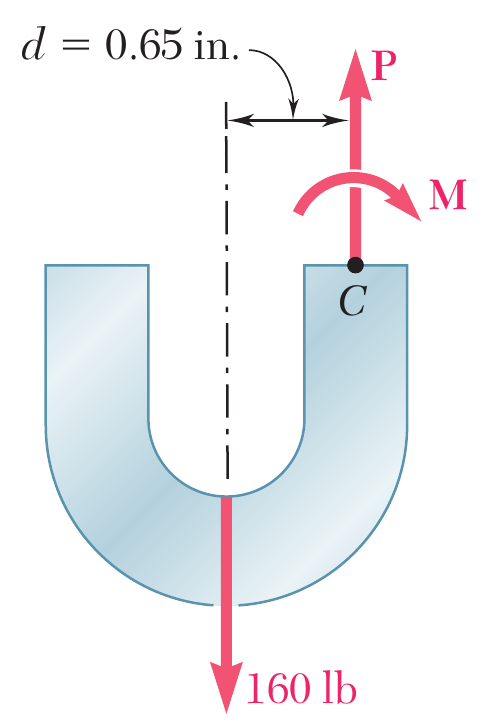
\includegraphics[width=0.7\linewidth,height=1.8cm,keepaspectratio]{Chap_4/fig_4_47.png}
    \column{0.49\textwidth}
      \small
      \begin{itemize}
        \item Ứng suất pháp do mô men uốn:
        \[
          I = \tfrac{1}{4}\pi c^4 = \tfrac{1}{4}\pi(6\,\mathrm{mm})^4
            = 1017{,}9\,\mathrm{mm}^4
        \]
        \[
          \sigma_m = \frac{Mc}{I}
            = \frac{(11{,}2\,\mathrm{N\cdot m})(0{,}006\,\mathrm{m})}{1017{,}9\times10^{-12}\,\mathrm{m}^4}
            = 66\,\mathrm{MPa}
        \]
      \end{itemize}
      \centering
      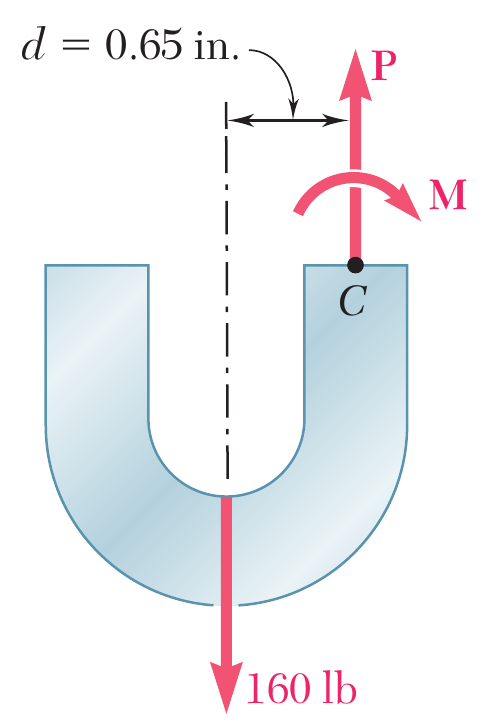
\includegraphics[width=0.8\linewidth,height=2.6cm,keepaspectratio]{Chap_4/fig_4_47.png}
  \end{columns}
\end{frame}
% ===========
\begin{frame}[t]{Ví dụ 4.07 (tiếp)}
  \begin{columns}[T]
    \column{0.58\textwidth}
      \small
      \begin{itemize}
        \setlength{\itemsep}{0.6em}
        \item Ứng suất kéo và nén lớn nhất:
        \[
          \sigma_t = \sigma_0 + \sigma_m = 6{,}2 + 66
          \qquad \boxed{\sigma_t = 72{,}2\,\mathrm{MPa}}
        \]
        \[
          \sigma_c = \sigma_0 - \sigma_m = 6{,}2 - 66
          \qquad \boxed{\sigma_c = -59{,}8\,\mathrm{MPa}}
        \]
        \item Vị trí trục trung hòa:
        \[
          0 = \frac{P}{A} - \frac{My_0}{I}
        \]
        \[
          y_0 = \frac{P}{A}\frac{I}{M}
            = (6{,}2\times10^{6}\,\mathrm{Pa})\frac{1017{,}9\times10^{-12}\,\mathrm{m}^4}{11{,}2\,\mathrm{N\cdot m}}
        \]
        \[
          \boxed{y_0 = 0{,}56\,\mathrm{mm}}
        \]
      \end{itemize}
    \column{0.40\textwidth}
      \centering
      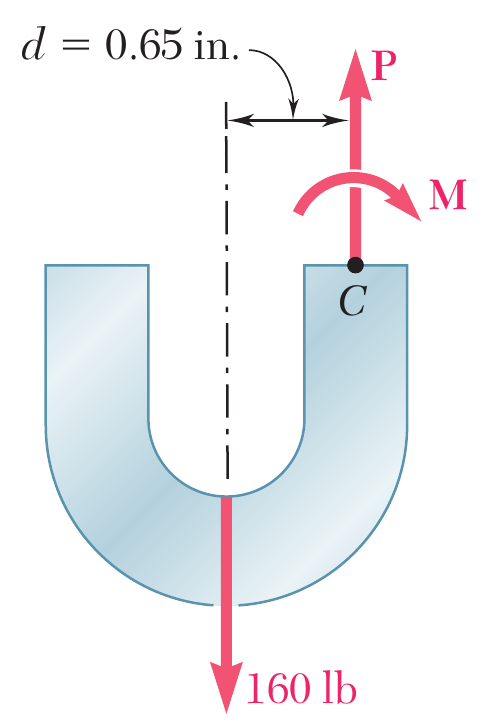
\includegraphics[width=\linewidth,height=5.5cm,keepaspectratio]{Chap_4/fig_4_47.png}
  \end{columns}
\end{frame}
% ===========
\section{Bài mẫu 4.8}
\begin{frame}[t]{Bài mẫu 4.8}
  \begin{columns}[T]
    \column{0.40\textwidth}
      \centering
      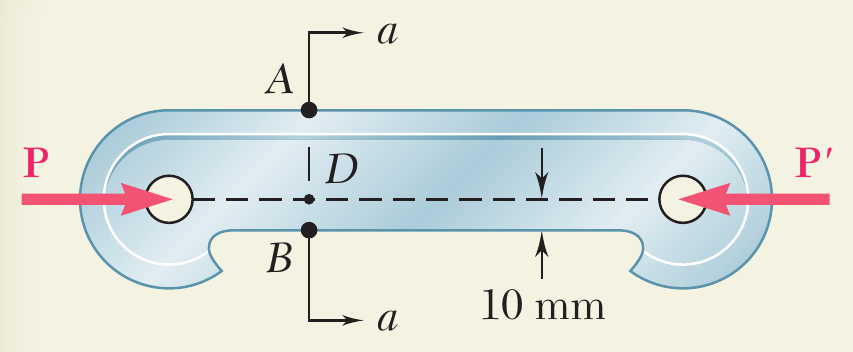
\includegraphics[width=\linewidth,height=2.9cm,keepaspectratio]{Chap_4/sp_4_8_a.png}\\[2pt]
      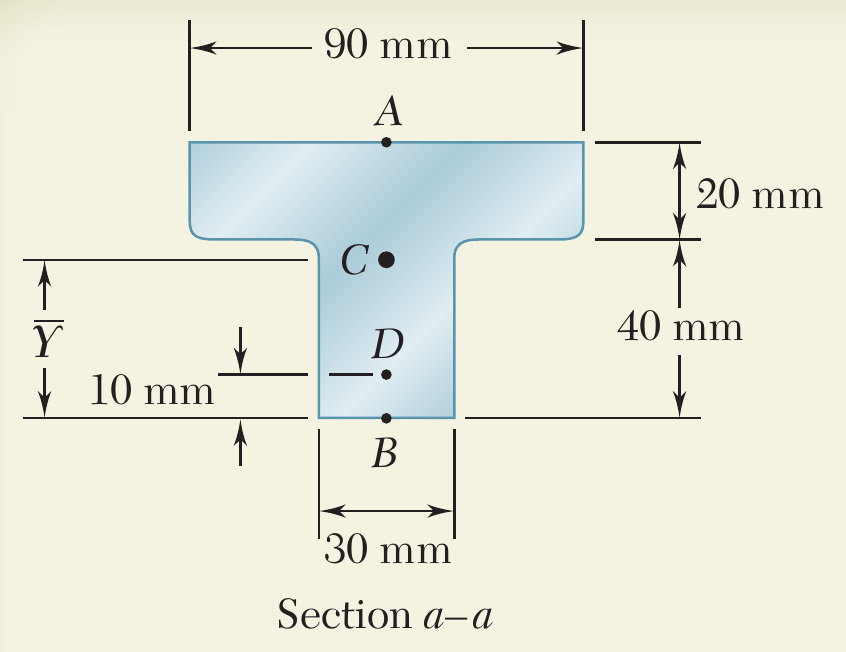
\includegraphics[width=\linewidth,height=2.9cm,keepaspectratio]{Chap_4/sp_4_8_b.png}
    \column{0.58\textwidth}
      \small
      Ứng suất cho phép lớn nhất của mắt nối bằng gang là 30 MPa khi kéo
      và 120 MPa khi nén. Xác định lực $P$ lớn nhất có thể tác dụng lên mắt
      nối.

      \vspace{0.3em}
      Từ Bài mẫu 4.2:
      $A = 3\times10^{-3}\,\mathrm{m}^2$, $\bar{Y} = 0{,}038\,\mathrm{m}$,
      $I = 868\times10^{-9}\,\mathrm{m}^4$

      \vspace{0.5em}
      \textbf{LỜI GIẢI:}
      \begin{itemize}
        \setlength{\itemsep}{0.3em}
        \item Xác định lực đúng tâm và mô men uốn tương đương.
        \item Cộng tác dụng ứng suất do lực đúng tâm và ứng suất do uốn.
        \item Tính các tải trọng tới hạn ứng với ứng suất kéo và nén cho
              phép.
        \item Tải trọng cho phép lớn nhất là giá trị nhỏ hơn trong hai tải
              trọng tới hạn.
      \end{itemize}
  \end{columns}
\end{frame}
% ===========
\begin{frame}[t]{Bài mẫu 4.8 (tiếp)}
  \begin{columns}[T]
    \column{0.62\textwidth}
      \footnotesize
      \begin{itemize}
        \setlength{\itemsep}{0.20em}
        \item Xác định lực đúng tâm và mô men uốn tương đương:
        \[
          d = 0{,}038 - 0{,}010 = 0{,}028\,\mathrm{m}
        \]
        $P$ = lực đúng tâm, \quad $M = Pd = 0{,}028P$ = mô men uốn
        \item Cộng tác dụng ứng suất do lực đúng tâm và do uốn:
        \[
          \sigma_A = -\frac{P}{A} + \frac{Mc_A}{I}
            = -\frac{P}{3\times10^{-3}} + \frac{(0{,}028P)(0{,}022)}{868\times10^{-9}}
        \]
        \[
          \sigma_A = +377P
        \]
        \[
          \sigma_B = -\frac{P}{A} - \frac{Mc_B}{I}
            = -\frac{P}{3\times10^{-3}} - \frac{(0{,}028P)(0{,}038)}{868\times10^{-9}}
        \]
        \[
          \sigma_B = -1559P
        \]
        \item Tính các tải trọng tới hạn ứng với ứng suất cho phép:
        \[
          \sigma_A = +377P = 30\,\mathrm{MPa} \qquad P = 79{,}6\,\mathrm{kN}
        \]
        \[
          \sigma_B = -1559P = -120\,\mathrm{MPa} \qquad P = 77{,}0\,\mathrm{kN}
        \]
        \item Tải trọng cho phép lớn nhất: \quad
              $\boxed{P = 77{,}0\,\mathrm{kN}}$
      \end{itemize}
    \column{0.36\textwidth}
      \centering
      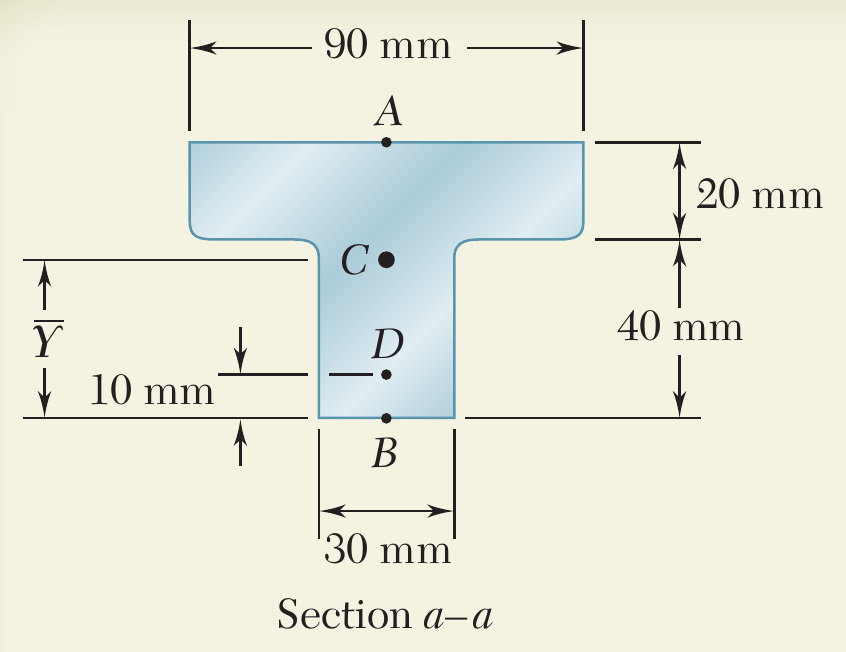
\includegraphics[width=\linewidth,height=2.5cm,keepaspectratio]{Chap_4/sp_4_8_b.png}\\[2pt]
      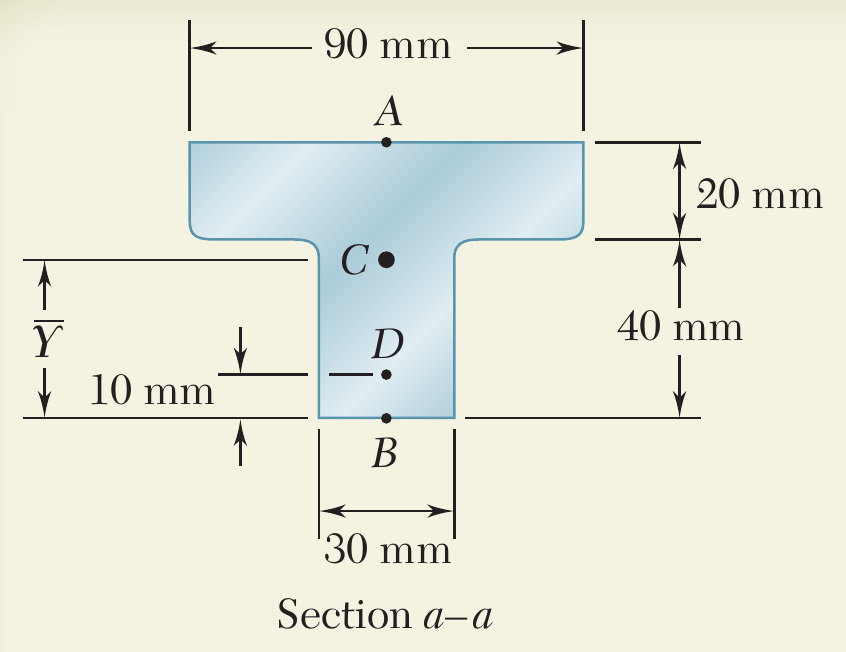
\includegraphics[width=\linewidth,height=2.5cm,keepaspectratio]{Chap_4/sp_4_8_b.png}
  \end{columns}
\end{frame}
% ===========
\section{Uốn không đối xứng}
\begin{frame}[t]{Uốn không đối xứng}
  \begin{columns}[T]
    \column{0.58\textwidth}
      \small
      \begin{itemize}
        \setlength{\itemsep}{0.3em}
        \item Phân tích uốn thuần túy ở trên chỉ giới hạn cho các cấu kiện
              chịu ngẫu lực uốn tác dụng trong mặt phẳng đối xứng.
        \item Cấu kiện vẫn đối xứng và bị uốn trong mặt phẳng đối xứng.
        \item Trục trung hòa của mặt cắt trùng với trục của ngẫu lực.
        \item Bây giờ ta xét các trường hợp ngẫu lực uốn không tác dụng
              trong mặt phẳng đối xứng.
        \item Không thể giả thiết cấu kiện bị uốn trong mặt phẳng của ngẫu
              lực.
        \item Nói chung, trục trung hòa của mặt cắt sẽ không trùng với trục
              của ngẫu lực.
      \end{itemize}
    \column{0.40\textwidth}
      \centering
      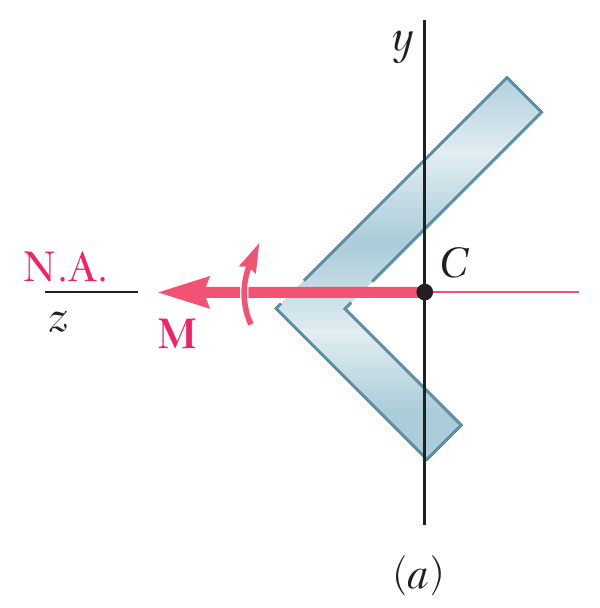
\includegraphics[width=0.49\linewidth,height=2.9cm,keepaspectratio]{Chap_4/fig_4_53.png}\hfill
      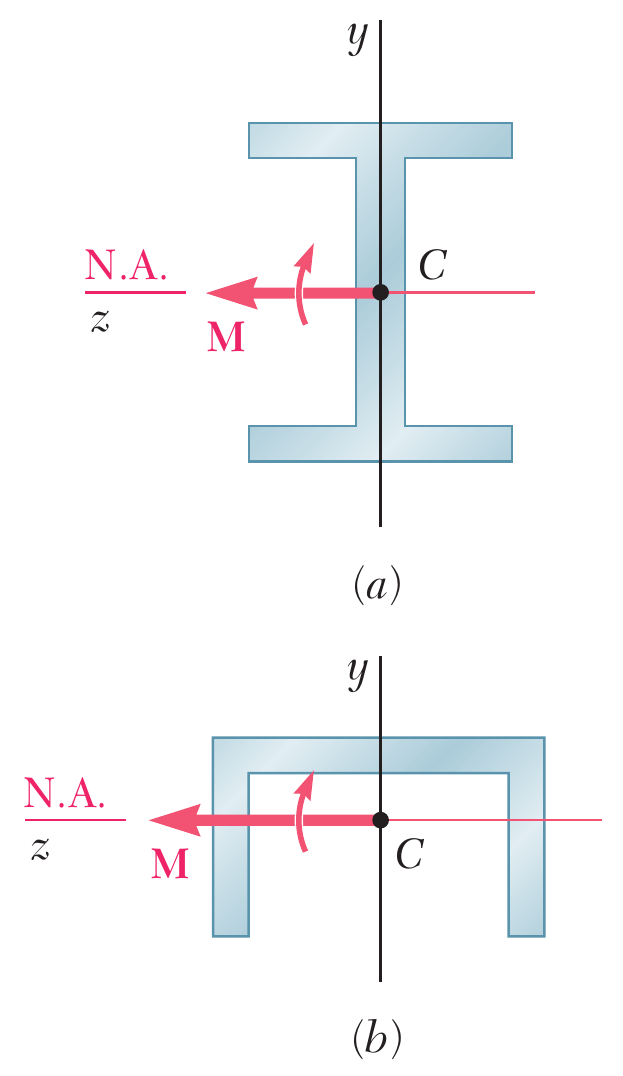
\includegraphics[width=0.49\linewidth,height=2.9cm,keepaspectratio]{Chap_4/fig_4_49.png}\\[2pt]
      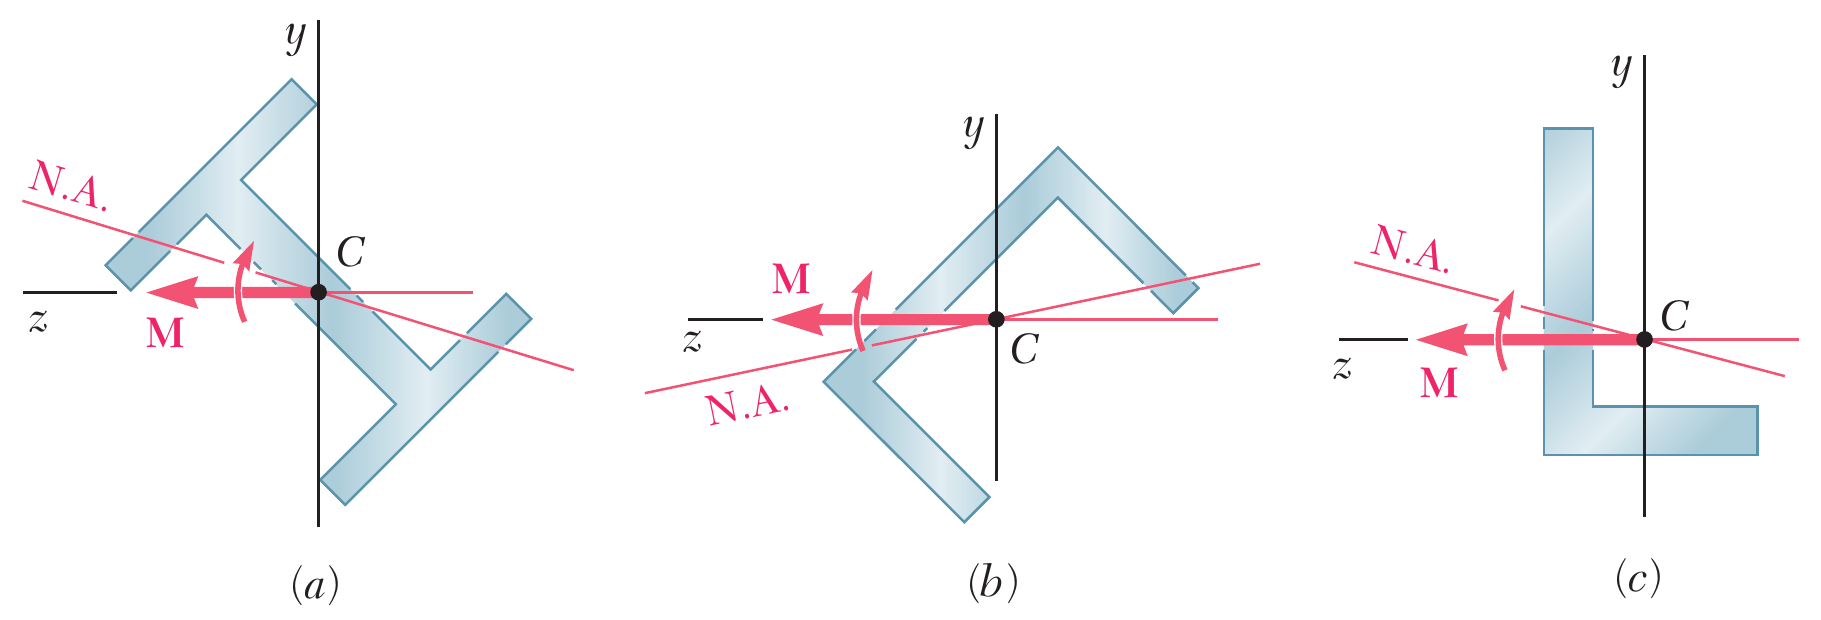
\includegraphics[width=0.49\linewidth,height=2.9cm,keepaspectratio]{Chap_4/fig_4_50.png}\hfill
      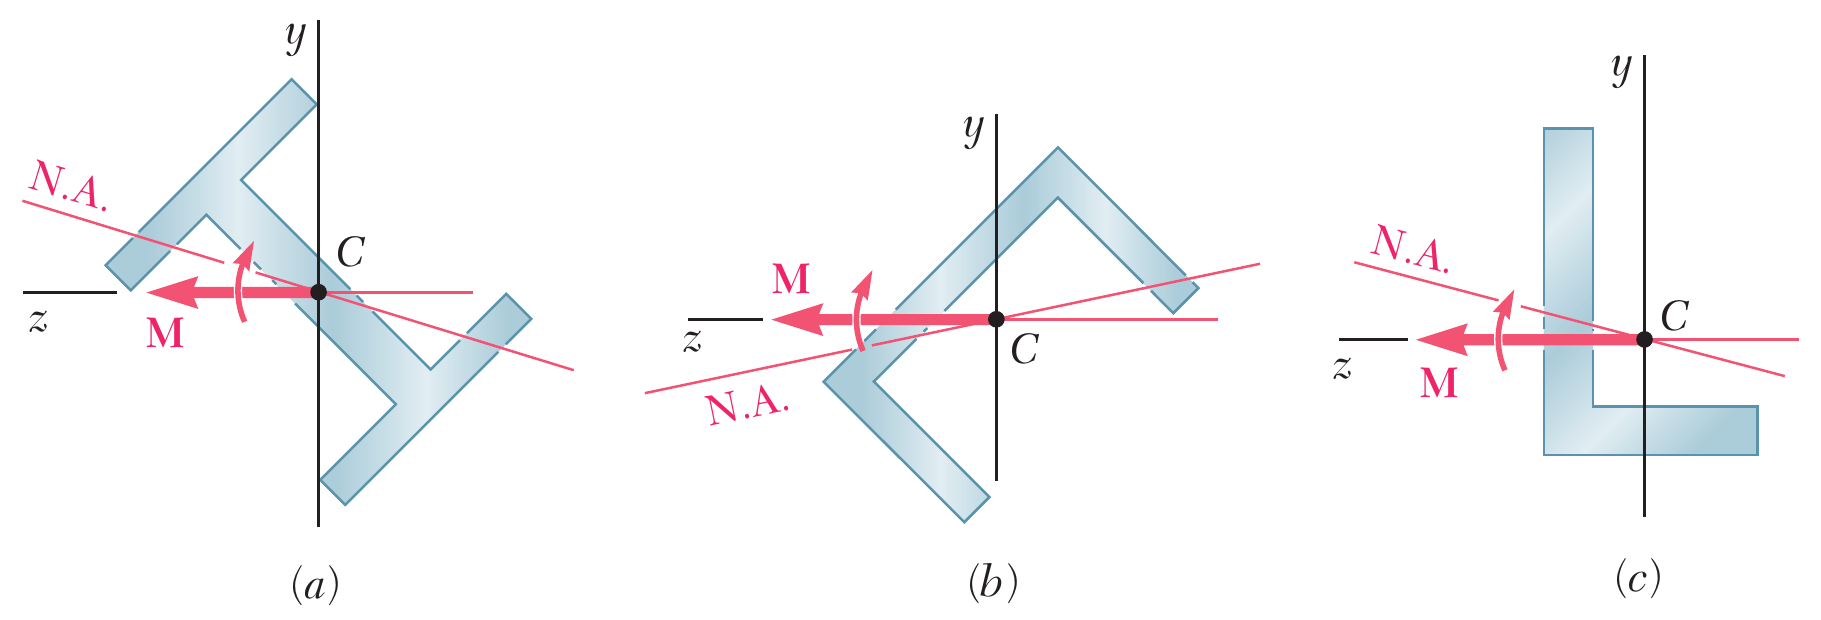
\includegraphics[width=0.49\linewidth,height=2.9cm,keepaspectratio]{Chap_4/fig_4_50.png}
  \end{columns}
\end{frame}
% ===========
\begin{frame}[t]{Uốn không đối xứng (tiếp)}
  \begin{columns}[T]
    \column{0.62\textwidth}
      \footnotesize
      Cần xác định điều kiện để trục trung hòa của mặt cắt có hình dạng bất
      kỳ trùng với trục của ngẫu lực như hình vẽ.
      \begin{itemize}
        \setlength{\itemsep}{0.3em}
        \item Hợp lực và mô men của phân bố các lực phân tố trên mặt cắt
              phải thỏa mãn:
              $F_x = 0 = M_y$, \quad $M_z = M$ = ngẫu lực tác dụng
        \item $\displaystyle 0 = F_x = \int\sigma_x\,dA
              = \int\left(-\frac{y}{c}\sigma_m\right)dA$
              \quad hay \quad $0 = \int y\,dA$\\
              trục trung hòa đi qua trọng tâm
        \item $\displaystyle M = M_z = -\int y\left(-\frac{y}{c}\sigma_m\right)dA$
              \quad hay \quad $M = \dfrac{\sigma_mI}{c}$, \quad
              $I = I_z$ = mô men quán tính\\
              xác định phân bố ứng suất
        \item $\displaystyle 0 = M_y = \int z\sigma_x\,dA
              = \int z\left(-\frac{y}{c}\sigma_m\right)dA$
              \quad hay \quad $0 = \int yz\,dA = I_{yz}$ = mô men quán tính
              ly tâm\\
              véc tơ ngẫu lực phải hướng theo một trục quán tính chính trung
              tâm
      \end{itemize}
    \column{0.36\textwidth}
      \centering
      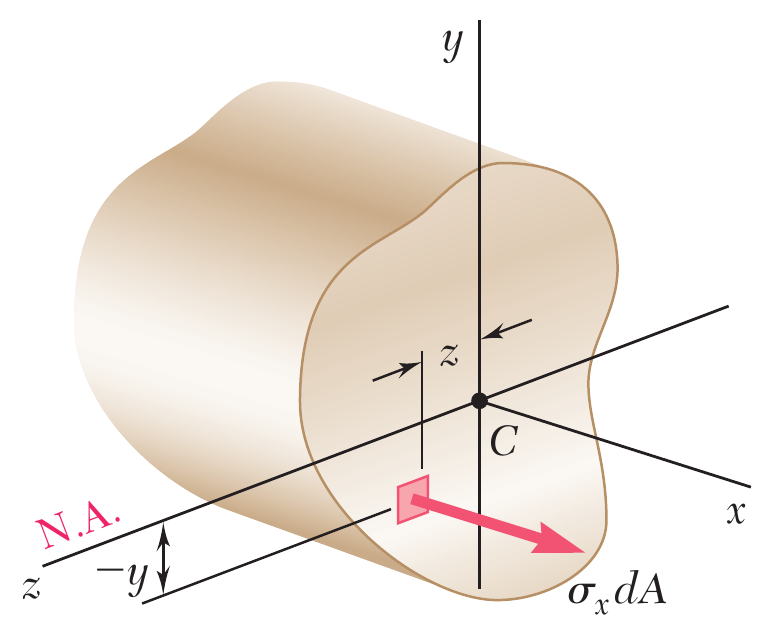
\includegraphics[width=\linewidth,height=5.5cm,keepaspectratio]{Chap_4/fig_4_51.png}
  \end{columns}
\end{frame}
% ===========
\begin{frame}[t]{Uốn không đối xứng (tiếp)}
  \begin{columns}[T]
    \column{0.58\textwidth}
      \footnotesize
      Nguyên lý cộng tác dụng được dùng để xác định ứng suất trong trường
      hợp uốn không đối xứng tổng quát nhất.
      \begin{itemize}
        \setlength{\itemsep}{0.20em}
        \item Phân tích véc tơ ngẫu lực thành các thành phần theo các trục
              quán tính chính trung tâm:
        \[
          M_z = M\cos\theta \qquad M_y = M\sin\theta
        \]
        \item Cộng tác dụng các phân bố ứng suất thành phần:
        \[
          \sigma_x = -\frac{M_zy}{I_z} + \frac{M_yz}{I_y}
        \]
        \item Dọc theo trục trung hòa:
        \[
          \sigma_x = 0 = -\frac{M_zy}{I_z} + \frac{M_yz}{I_y}
        \]
        \[
          0 = -\frac{(M\cos\theta)y}{I_z} + \frac{(M\sin\theta)z}{I_y}
        \]
        \[
          \tan\phi = \frac{y}{z} = \frac{I_z}{I_y}\tan\theta
        \]
      \end{itemize}
    \column{0.40\textwidth}
      \centering
      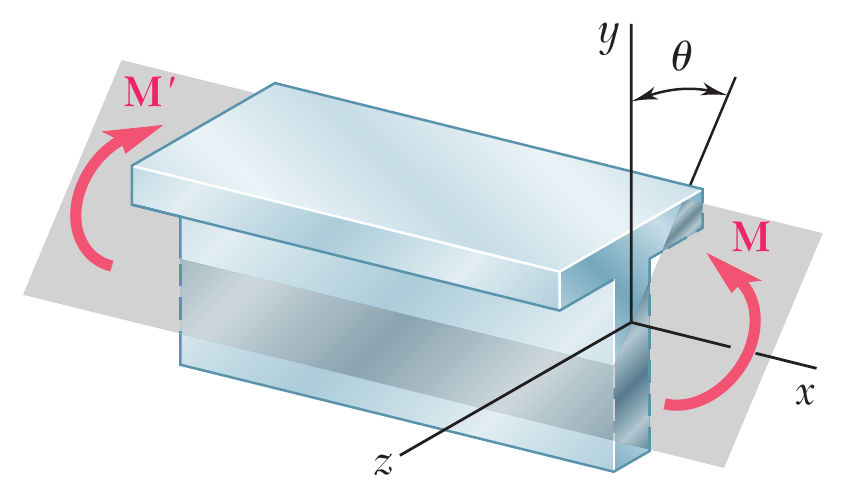
\includegraphics[width=0.49\linewidth,height=2.5cm,keepaspectratio]{Chap_4/fig_4_54.png}\hfill
      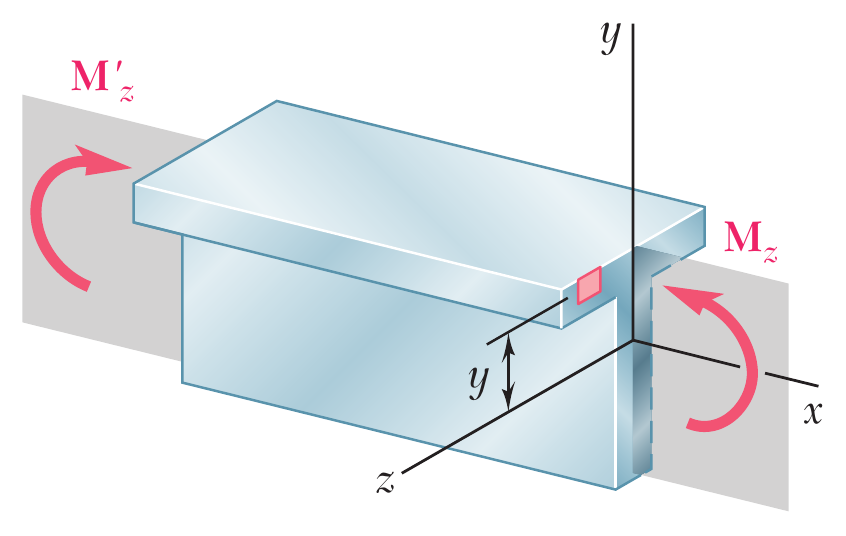
\includegraphics[width=0.49\linewidth,height=2.5cm,keepaspectratio]{Chap_4/fig_4_56.png}\\[2pt]
      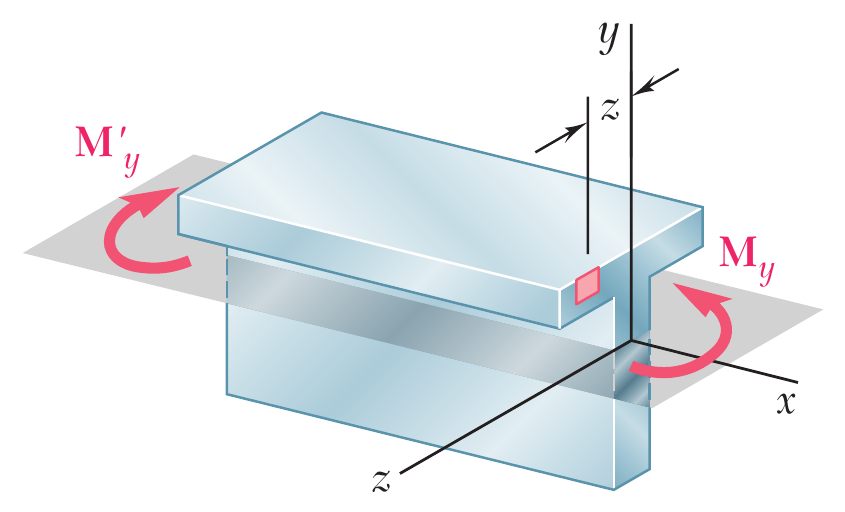
\includegraphics[width=0.49\linewidth,height=2.5cm,keepaspectratio]{Chap_4/fig_4_57.png}\hfill
      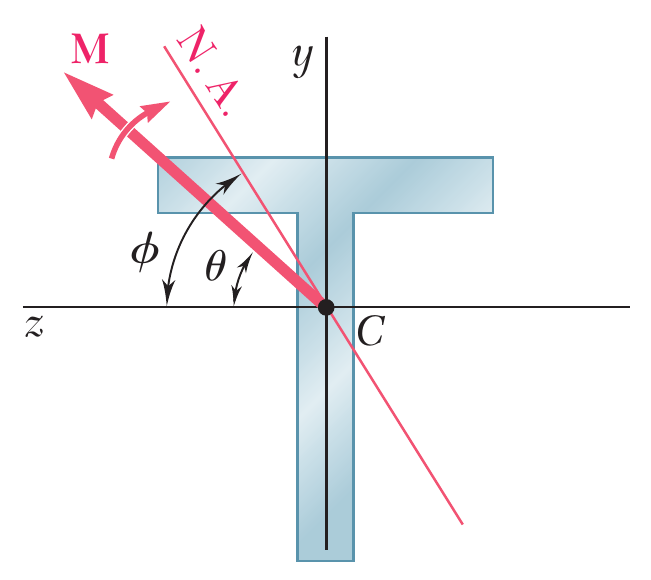
\includegraphics[width=0.49\linewidth,height=2.5cm,keepaspectratio]{Chap_4/fig_4_59.png}
  \end{columns}
\end{frame}
% ===========
\section{Ví dụ 4.08}
\begin{frame}[t]{Ví dụ 4.08}
  \begin{columns}[T]
    \column{0.40\textwidth}
      \centering
      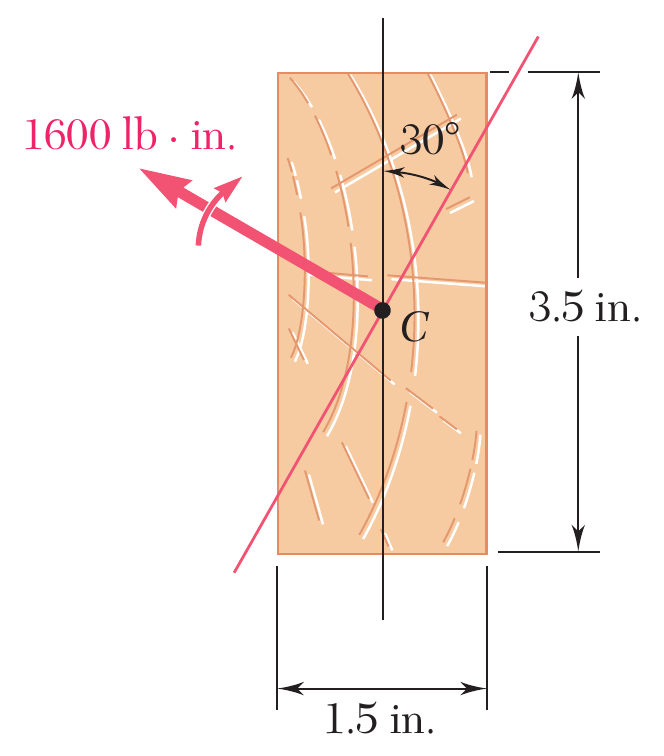
\includegraphics[width=\linewidth,height=4.7cm,keepaspectratio]{Chap_4/fig_4_60.png}
    \column{0.58\textwidth}
      \footnotesize
      Một ngẫu lực $180\,\mathrm{N\cdot m}$ tác dụng lên dầm gỗ chữ nhật
      trong mặt phẳng hợp với phương thẳng đứng một góc $30^\circ$. Xác định
      (a) ứng suất lớn nhất trong dầm, (b) góc hợp bởi trục trung hòa và mặt
      phẳng nằm ngang.

      \vspace{0.5em}
      \textbf{LỜI GIẢI:}
      \begin{itemize}
        \setlength{\itemsep}{0.20em}
        \item Phân tích véc tơ ngẫu lực thành các thành phần theo các trục
              quán tính chính trung tâm và tính ứng suất lớn nhất tương ứng:
              \[ M_z = M\cos\theta \qquad M_y = M\sin\theta \]
        \item Tổ hợp ứng suất từ các phân bố ứng suất thành phần:
              \[ \sigma_x = \frac{M_zy}{I_z} + \frac{M_yz}{I_y} \]
        \item Xác định góc của trục trung hòa:
              \[ \tan\phi = \frac{y}{z} = \frac{I_z}{I_y}\tan\theta \]
      \end{itemize}
  \end{columns}
\end{frame}
% ===========
\begin{frame}[t]{Ví dụ 4.08 (tiếp)}
  \begin{columns}[T]
    \column{0.60\textwidth}
      \scriptsize
      \begin{itemize}
        \setlength{\itemsep}{0.15em}
        \item Phân tích véc tơ ngẫu lực thành các thành phần và tính ứng suất
              lớn nhất tương ứng:
        \[
          M_z = (180)\cos30^\circ = 155{,}9\,\mathrm{N\cdot m}
        \]
        \[
          M_y = (180)\sin30^\circ = 90\,\mathrm{N\cdot m}
        \]
        \[
          I_z = \tfrac{1}{12}(40)(90)^3 = 2{,}43\times10^{6}\,\mathrm{mm}^4
        \]
        \[
          I_y = \tfrac{1}{12}(90)(40)^3 = 0{,}48\times10^{6}\,\mathrm{mm}^4
        \]
        Ứng suất kéo lớn nhất do $M_z$ xảy ra dọc theo $AB$:
        \[
          \sigma_1 = \frac{M_zy}{I_z}
            = \frac{(155{,}9)(0{,}045)}{2{,}43\times10^{-6}}
            = 2{,}89\,\mathrm{MPa}
        \]
        Ứng suất kéo lớn nhất do $M_y$ xảy ra dọc theo $AD$:
        \[
          \sigma_2 = \frac{M_yz}{I_y}
            = \frac{(90)(0{,}020)}{0{,}48\times10^{-6}}
            = 3{,}75\,\mathrm{MPa}
        \]
        \item Ứng suất kéo lớn nhất do tải trọng tổ hợp xảy ra tại $A$:
        \[
          \sigma_{\max} = \sigma_1 + \sigma_2 = 2{,}89 + 3{,}75
          \qquad \boxed{\sigma_{\max} = 6{,}64\,\mathrm{MPa}}
        \]
      \end{itemize}
    \column{0.38\textwidth}
      \centering
      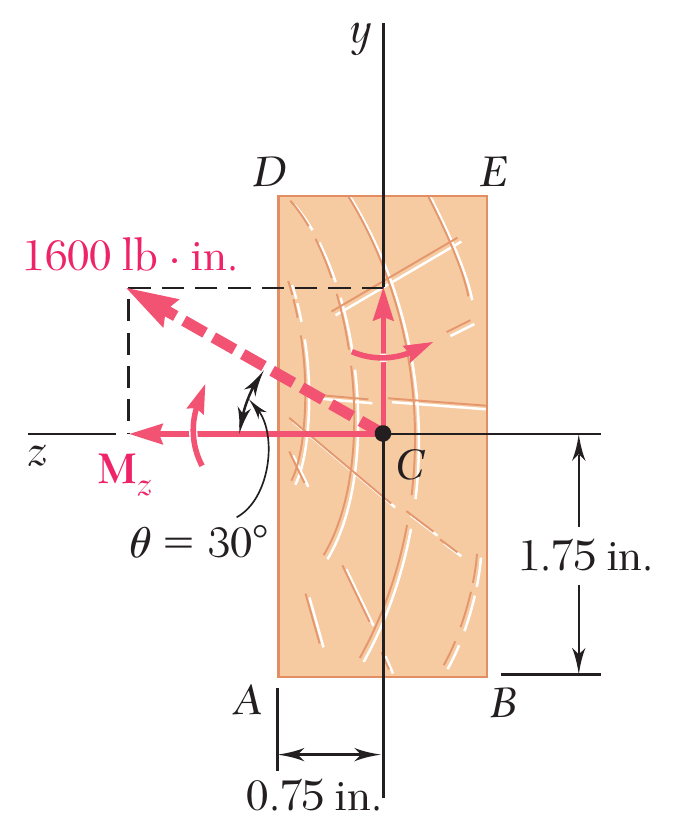
\includegraphics[width=\linewidth,height=4.7cm,keepaspectratio]{Chap_4/fig_4_61.png}
  \end{columns}
\end{frame}
% ===========
\begin{frame}[t]{Ví dụ 4.08 (tiếp)}
  \begin{columns}[T]
    \column{0.56\textwidth}
      \small
      \begin{itemize}
        \item Xác định góc của trục trung hòa:
      \end{itemize}
      \[
        \tan\phi = \frac{I_z}{I_y}\tan\theta
          = \frac{2{,}43\times10^{-6}\,\mathrm{m}^4}{0{,}48\times10^{-6}\,\mathrm{m}^4}\tan30^\circ
          = 2{,}9
      \]
      \[
        \boxed{\phi = 71^\circ}
      \]
    \column{0.42\textwidth}
      \centering
      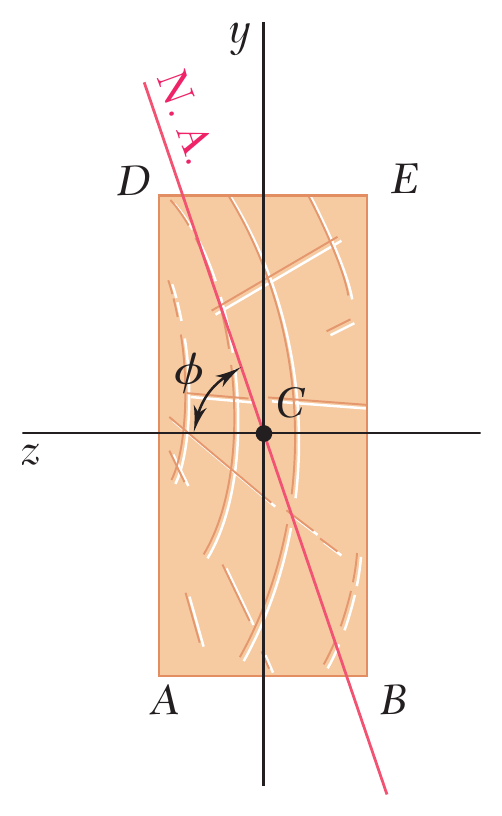
\includegraphics[width=\linewidth,height=5.5cm,keepaspectratio]{Chap_4/fig_4_62.png}
  \end{columns}
\end{frame}
% ===========
\section{Trường hợp tổng quát của tải trọng dọc trục lệch tâm}
\begin{frame}[t]{Trường hợp tổng quát của tải trọng dọc trục lệch tâm}
  \begin{columns}[T]
    \column{0.58\textwidth}
      \small
      \begin{itemize}
        \setlength{\itemsep}{0.6em}
        \item Xét một cấu kiện thẳng chịu các lực lệch tâm bằng nhau và
              ngược chiều.
        \item Lực lệch tâm tương đương với hệ gồm một lực đúng tâm và hai
              ngẫu lực:
        \[
          P = \text{lực đúng tâm} \qquad M_y = Pa \qquad M_z = Pb
        \]
        \item Theo nguyên lý cộng tác dụng, phân bố ứng suất tổng hợp là:
        \[
          \sigma_x = \frac{P}{A} - \frac{M_zy}{I_z} + \frac{M_yz}{I_y}
        \]
        \item Nếu trục trung hòa nằm trên mặt cắt, nó có thể được xác định
              từ:
        \[
          \frac{M_z}{I_z}y - \frac{M_y}{I_y}z = \frac{P}{A}
        \]
      \end{itemize}
    \column{0.40\textwidth}
      \centering
      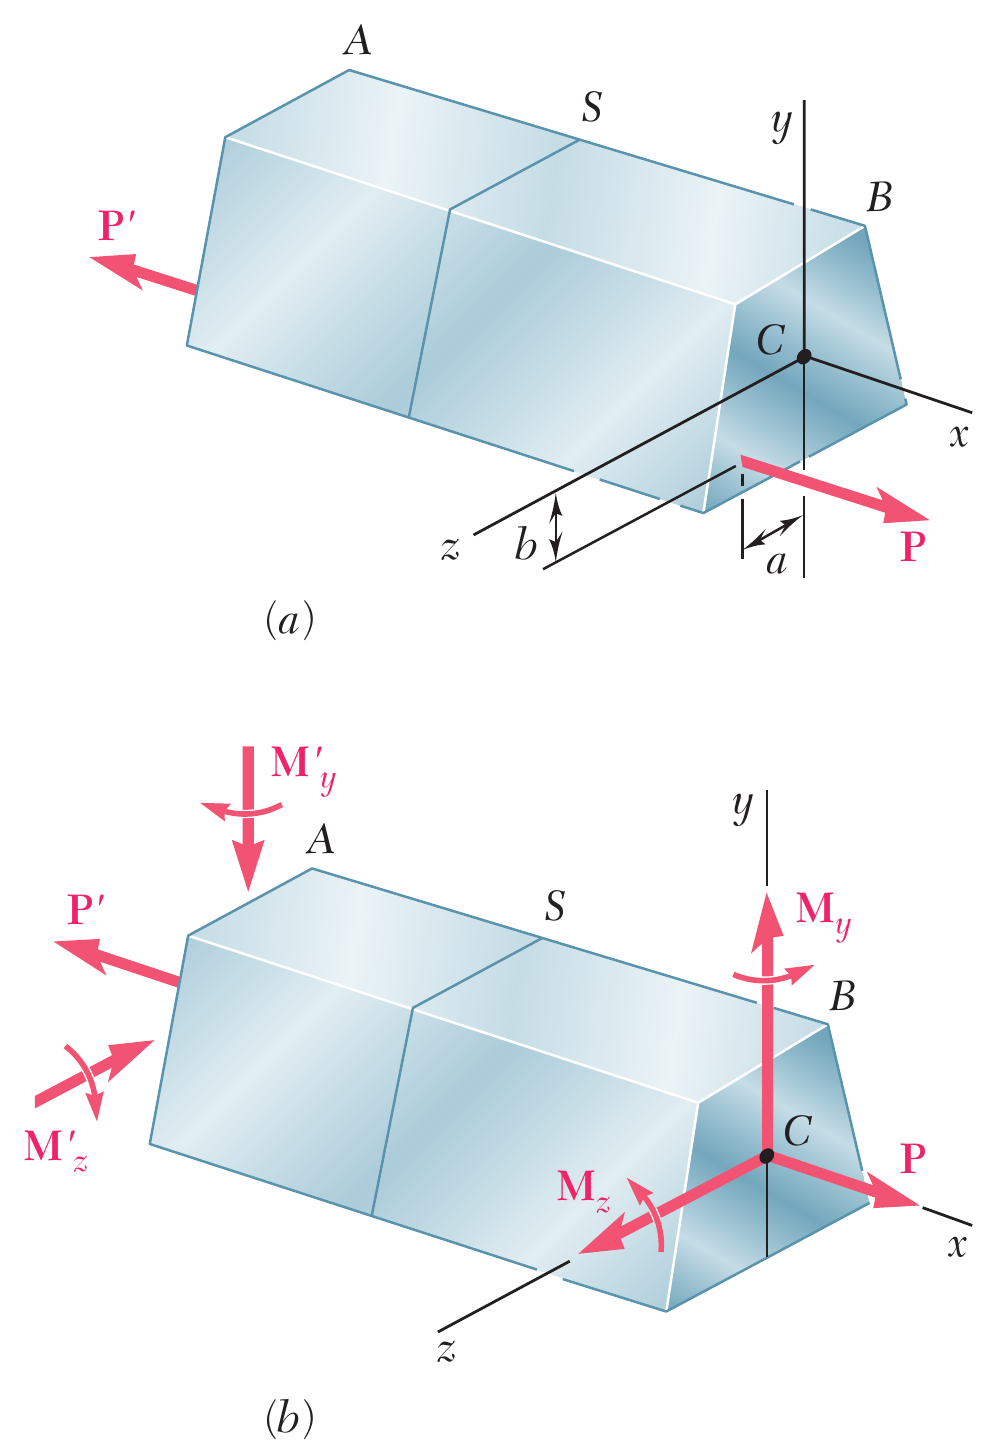
\includegraphics[width=\linewidth,height=2.9cm,keepaspectratio]{Chap_4/fig_4_64.png}\\[2pt]
      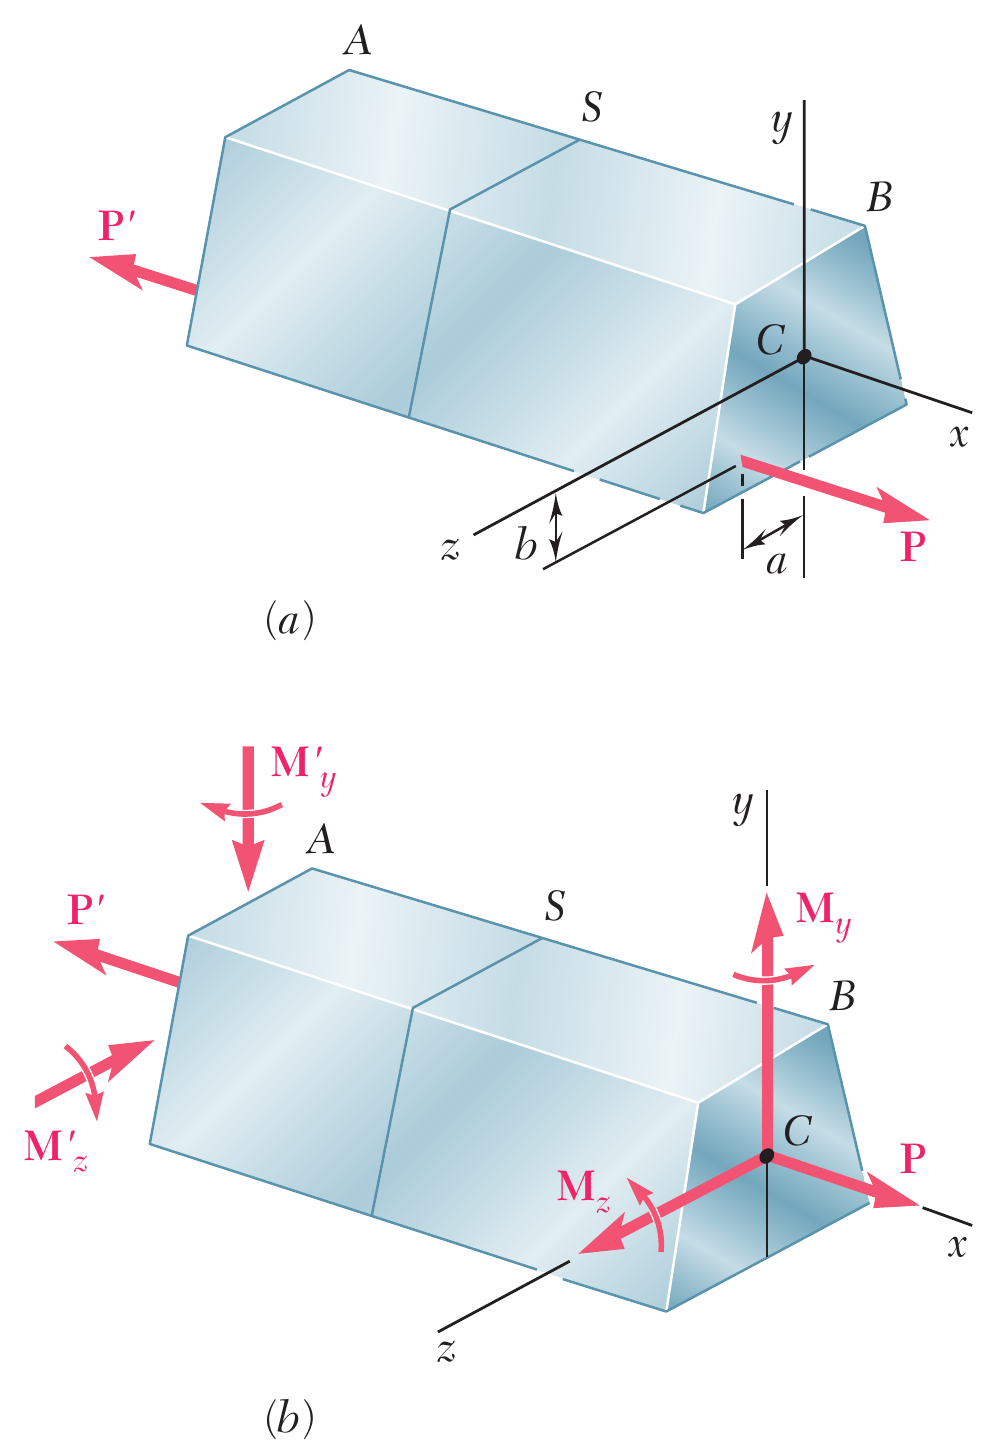
\includegraphics[width=\linewidth,height=2.9cm,keepaspectratio]{Chap_4/fig_4_64.png}
  \end{columns}
\end{frame}

\end{document}
